%% Template for Master thesis
%% ===========================
%%
%% You need at least KomaScript v3.0.0,
%% e.g. available in Texlive 2009
\documentclass  [
  paper    = a4,
  BCOR     = 10mm,
  twoside,
  fontsize = 12pt,
  fleqn,
  toc      = bibnumbered,
  toc      = listofnumbered,
  numbers  = noendperiod,
  headings = normal,
  listof   = leveldown,
  version  = 3.03
]                                       {scrreprt}

% used pagages
%\usepackage[margin=10pt,font=small,labelfont=bf,labelsep=endash]{caption}
\usepackage     [utf8]          {inputenc}
\usepackage     [T1]            {fontenc}
\usepackage                     {color}
\usepackage                     {amsmath}
\usepackage                     {graphicx}
\usepackage     [english]       {babel}
\usepackage                     {natbib}
\usepackage                     {hyperref}
\usepackage						{cleveref}
\usepackage						{subfigure}
\usepackage						{multirow}
\usepackage						{booktabs} % Allows the use of \toprule, \midrule and \bottomrule in tables
\usepackage						{multicol} % Required for creating multiple columns in slides
\usepackage		[version=4]		{mhchem}
% links
\definecolor{darkblue}{rgb}{0.0,0.0,0.4}
\definecolor{darkgreen}{rgb}{0.0,0.4,0.0}
\hypersetup{
    colorlinks,
    linkcolor=black,
    citecolor=darkgreen,
    urlcolor=darkblue
}
%\renewcommand{\partname}{}
%\renewcommand{\thepart}{}

\begin{document}
  %% title pages similar to providet template instead of maketitle
  %% this will generate title pages similar to the template provided
%% by the Department of Physics and Astronomy Heidelberg
%%
%% More information:
%% http://www.physik.uni-heidelberg.de/aktuelles/studium/
%% (PDF link: ...studium/download/145/Vorlage_Diplomarbeit_Formular.pdf)

%% Titleintro
\thispagestyle{empty}
\begin{center}
  \renewcommand{\baselinestretch}{2.00}
  \Large\sffamily
  Department of Physics and Astronomy\\
  \large University of Heidelberg
  \par\vfill\normalfont
  Master thesis\\
  in Physics\\
  submitted by\\
  Elsa  Wilken\\
  born in Hamburg\\
  2018
\end{center}
\newpage

%% Titlepage
\thispagestyle{empty}
\begin{center}
  \renewcommand{\baselinestretch}{2.00}
  \Large\bfseries\sffamily
    Retrieval Advances of BrO/\ce{SO2}              \\
    Molar Ratios from NOVAC\\
  \par
  \vfill
  \large\normalfont
  This Master thesis has been carried out by Elsa Wilken\\
  at the\\
  Institute for Environmental Physics, University of Heidelberg, Germany\\
  under the supervision of\\
  Prof. Ulrich Platt,\\
  Dr. Nicole Bobrowski,\\
  Florian Dinger
  %% additionally insert second supervisor here if carrying out an
  %% external diploma thesis. Reduce vspace in L. 44 accordingly.
\end{center}\par
\vspace{5\baselineskip}

% reset baselinestretch
\renewcommand{\baselinestretch}{1.00}\normalsize % or english title page
  %% Abstract page
%% =============
%%
%% Content of abstract pages has been put into seperate pages to simplify
%% word counting. Use e.g. the unix command
%%   wc abstract-ger.tex
%% or
%%   wc abstract-eng.tex
%% to get the number of words contained in these files.
\thispagestyle{empty}
\begin{center}
  \begin{minipage}[c][0.48\textheight][b]{0.9\textwidth}
    \small
    \textbf{Optimierte Bestimmung des molaren BrO/\ce{SO2} Verhältnisses aus NOVAC Daten
    }\par
    \vspace{\baselineskip}
    %% Latex markup und Zitate funktionieren auch hier


Die Messung der absoluten Menge und von Konzentrationsverhältnissen vulkanischer Gas Emissionen geben Einsicht in magmatische Prozesse. Das Network for Observation of Volcanic and Atmospheric Change (NOVAC) besteht aus einem System von automatisierten UV-Spektrometern, welche die Gas Emissionen der Vulkane aufzeichnen. Die Emission von BrO und \ce{SO2} kann mithilfe von Differenzieller optischer Absorptionsspektroskopie (DOAS) aus den aufgenommen Spekren bestimmt werden wobei die optische Absorption in der Fahne mit einem Reference Spectrum verglichen wird. Dies setzt voraus, dass das Reference Spectrum frei von Vulkanische Gasen ist. Typischerweise wird das Reference Spectrum für einen Scan bei einem Elevationswinkel aufgenommen welcher welcher so gewählt wird dass das Instrument nicht in die Fahne schaut. Es hat sich jedoch gezeigt, dass auch diese Spektren noch durch Vulkanische Emissionen verunreinigt sein können. Als alternative Referenzspektren könnten 1) ein theoretisches Solar Atlas Spektrum oder 2) ein nicht verunreinigtes Referenz Spektrum des selben Messgeräts dienen. Option 1) hat den Nachteil einer verringerten Messgenauigkeit, da Instrumenteneffekte hier modelliert werden müssen und ist daher nur für das typischerweise in hoher Konzentration vorkommende \ce{SO2} anwendbar. Option 2) setzt voraus, dass das Referenzspektrum unter ähnlichen Wetter- und Strahlungsbedingungen aufgenommen wurde. Wir verwenden die erste Methode um (\ce{SO2}) Kontaminierung zu identifizieren und greifen für die Bestimmung der Gas Konzentration auf die zweite Methode zurück um eine hohe Qualität der Messung sicher zu stellen. Im Folgenden stellen wir unsere Methode für NOVAC Daten von den Vulkanen Tungurahua und Nevado Del Ruiz vor.
  \end{minipage}\par
  \vfill
  \begin{minipage}[c][0.48\textheight][b]{0.9\textwidth}
    \small
    \textbf{Retrieval advances of BrO/\ce{SO2} molar ratios from NOVAC
    }\par
    \vspace{\baselineskip}
    %% Latex markup and citations may be used here

%Measurements of magnitude and composition of volcanic gas emissions allow insights in magmatic processes. Within the Network for Observation of Volcanic and Atmospheric Change(NOVAC) automatically scanning UV-spectrometers are monitoring gas emission at volcanoes. The emissions of BrO and \ce{SO2} can be retrieved from the recorded spectra by applying Differential Optical Absorption Spectroscopy(DOAS) and comparing the optical absorption of the volcanic plume to the background. Therefore, the background spectrum must not be affected by volcanic influence. Conventionally, the background spectrum is taken from the same scan but from an elevation angle which has been identified to be outside of the volcanic plume. However, experience shows those background spectra can still be contaminated by volcanic gases.  Alternatively, background spectra can be derived from 1) a theoretical solar atlas spectrum or 2) a volcanic-gas-free background spectrum recorded by the same instrument at another time. 1) comes with a drawback of reduced precision, as the instrumental effects have to be modeled and added to the retrieval. For 2), the alternative background spectrum should be recorded at similar conditions with respect to meteorology and radiation. We use the first option to check for contamination and the second to evaluate the spectra to maintain a good fit quality. We present our approach and its results when applied on NOVAC data from Tungurahua and Nevado del Ruiz.

Measurements of magnitude and composition of volcanic gas emissions allow insights into magmatic processes. In this thesis, the concentration ratio of BrO and \ce{SO2} is analyzed. The measurements are performed with scanning UV-spectrometers provided by the "Network for Observation of Volcanic and Atmospheric Change (NOVAC)".
The concentrations are then retrieved by applying Differential Optical Absorption Spectroscopy (DOAS).
For this purpose, especially weak absorbers like BrO require a gas-free reference spectrum to eliminate the Fraunhofer structures.
However, with the conventional evaluation approach, it is still possible that the chosen same-time-reference spectra are contaminated. Alternative reference spectra could be (1) a theoretical solar atlas spectrum or (2) a temporal shifted uncontaminated reference spectrum which is recorded by the same instrument. (1) comes with the drawback of a decreased measurement precision, as instrumental effects must be modeled, while (2) only works with a reference that is recorded under similar conditions as the measurement spectrum. In this work, a new approach is presented which uses (1) for the identification of (\ce{SO2}) contamination and (2) for the actual measurement of the gas concentration. The novel approach sidesteps the systematic underestimation of the concentration and increases the amount of reliable data by approximately 30\%. Moreover, we are able to prove the occurrence of BrO contamination.
  \end{minipage}
\end{center}


  \tableofcontents
  %% Put your contents here
	\chapter{Introduction}	
	
%% Introduction page
%% =============
%%
Volcanic activities on Earth have  always shaped the earth surface and influenced atmospheric processes. Volcanoes are often particularly recognized by their dramatic consequences of a major volcanic eruption. But volcanoes influence our lives in more than this way. Volcanic gases can effect the weather (timescales of days to weeks) or the climate (timescales of months to years) \cite{schmidt2015volcanismarticle}.
Examples are the lake eruption in Iceland (1783-1784) followed by a very hot summer and a cold winter in central Europa \cite{thordarson2003atmospheric} and the Tambora eruption, indonesia in 1815 which caused the "year without summer" in 1816.\\
%
\newline
%
Considering the plate tectonics of earth  most volcanoes are caused by diverging or converging of the continental plates and therefore located at the margins of the continental plates.
Another possibility for occurrence of volcanoes is the the interior of continental or oceanic shelves. \cite{schmincke2000vulkanismus}\\
The most abundant volatile species released during a volcanic eruption are water vapour (H$_2$O; relative amount of the plume: 50\%-90\%) and carbon dioxide (CO$_2$; relative amount of the plume: 1\%-40\%) \cite{platt2015quantification}. But the short effects of those two gases are rather low since there effect on atmospheric composition is negligibly due to the high abundance of atmospheric H$_2$O and CO$_2$. But on timescales of the age of the earth the volcanic emission of H$_2$O and CO$_2$ are the source of our current atmosphere. \cite{schmidt2015volcanism}\\ 
A typically volcanic plume consists of many different gases alongside H$_2$O and CO$_2$  sulfur dioxide (SO$_2$) contributes with 1\%-25\% to the plume, hydrogen sulfide (H$_2$S) with 1\%-10\% and hydrogen chloride with (HCl) 1\%-10\%. Furthermore there are trace gases for example carbon disulfide (CS$_2$), carbon sulfide (COS) carbon monoxide (CO) hydrogen fluoride (HF) and hydrogen bromide (HBr) \cite{platt2015quantification}\\
%
A decrease of stratospheric ozone (O$_3$) has been observed after the eruption of  El Chickon in 1982 and the eruption of mount Pinatubo 1991. A depletion stratospheric O$_3$ results in ozone holes. The depletion comes from volcanic aerosols which serve anthropogenic chlorine/bromine into more reactive forms \cite{solomon1998ozone}. 
%
Volcanic gases can alter the radiative balance of the earth in timescales relevant for climate change due to scatter and absorption of solar radiation \cite{schmidt2015volcanism}.\\
%
The gas composition of the volcano plume change with activity and could be a indication for the processes inside the earth.\\ 
%
In this work we are particularly interested in the ratio of BrO and SO$_2$. The halogen sulfur ratio is a proxy for volcanic processes. Therefore we make the assumption
that the ratio of BrO and SO2 contains informations about its degassing source depth. A change in BrO/SO2 prior to eruption was observed at Etna and Nevado del Ruiz.\\
%
\newline
%
To gain further knowledge about the volcanoes the Network for Observation of Volcanic and Atmospheric Change (NOVAC) was installed. NOVAC is a Network of DOAS Instruments located next to about 30 volcanoes in America, Africa and Europe. At every Volcano there are two to four DOAS Instruments installed, recording record back-scattered solar radiation spectra at different viewing angles.\\
NOVAC is a network which produces a large amount of data and we have the chance to evaluate long time periods which is a unique opportunity to study correlations of the trace gases.\\
Since the conditions at volcanoes are rough, the instruments need to be rather simple to keep the maintenance cheap and to assure a longer lifetime of the instruments. So we need to waive on temperature stabilization even at the expense of the quality of the data.\\
%
\newline
%
One possibility to measure the volcanic trace gases is to use Differential Optical Absorption Spectroscopy \cite{platt2008differential}. DOAS exploit the wavelength dependency of the absorption of light. Here the gas emissions can be retrieved
from the quotient of the absorption signal of the volcanic plume and a
reference region. This will be explained in a further chapter.\\
%
\newline
%
The reference region, is usually treated as free of
volcanic trace gases. If the reference region is for any reason
contaminated by volcanic trace gases, the reference spectrum has to be
replaced by a volcanic-gas-free reference. Alternative spectra could be for example a
theoretical solar atlas spectrum or a volcanic-gas-free reference
spectrum recorded in the temporal proximity(eg. a day before) by the same instrument. 
The first option comes with the drawback of reduced precision, as the
instrumental effects have to be modeled and added to the retrieval. The
reduction in precision is acceptable for the SO2 retrieval, but not suitable
for a BrO retrieval because then most data would be below the detection
limit. For the second option, the alternative reference spectrum should
have been recorded at similar conditions with respect to meteorology and
radiation as well as in the temporal proximity due to instrumental changes
with time and ambient conditions. We combined both options in order to
achieve both, enhanced accuracy but still maximum possible precision of
the SO2 and BrO retrievals. We present an algorithm which finds the
optimal reference spectrum automatically. As first step, a possible SO2
contamination of the standard reference is checked by a comparison with
the theoretical solar atlas. If a contamination is detected, as second step,
the algorithm picks a volcanic-gas-free reference (beforehand
automatically checked for contamination) from another scan.\\
%
\newline
%
In this work we are mainly dealing with data from Tungurahua in Ecuador in the timespan of 01.08.2008 to 30.07.2009. Later on, we will also show the results of Nevado del Ruiz a volcano located in Colombia.\\
    \part{Theoretical Background}
\chapter{Volcanism and volcanic chemistry}
\section{Volcanism}
The high thermal energy in the deep interior of the earth is mostly well separated from the earth’s surface by the earth’s crust. A volcano is geological structure that allows magma to reach the earth’s surface. Such a phenomenon can occur in various ways. In the following paragraphs the different types of volcanoes are described.
\paragraph{ Mid-ocean ridge volcanism}
The mid-ocean ridge volcanism can be traced back to tectonic processes of oceanic plates. The spreading of two plates, that are pulled apart, leads to a thinning of the oceanic earth crust. This way solid material from the upper mantel (lower than 100 km) can ascend to depths of approximately 50 km. As the pressure at this depth is much lower, the mantle material starts to melt to basaltic magma that fills the gap between the two plates.
\paragraph{ Continental rift zone volcanism}
Similar to mid-ocean ridge volcanism continental rift zone volcanism results from two continental plate are pulled apart.
\paragraph{ Subduction zone volcanoes}
Subduction zone volcanoes occur if an oceanic plate converges under another plate (oceanic or continental). This way the descending plate penetrate into the lower mantle. At a depth of 80-150 km the water of this plate evaporates and rises and causes the mantle material above to melt. The resulting water-rich magma mainly consists of andesite. Subduction zone volcanoes are known for their violent eruptions caused by the low viscosity magma.
\paragraph{ Hot-spot volcanoes} Hot-spot volcanoes occur on continental or oceanic plates. This type of volcanoes arises from a hot spot at the coremantle boundary inside Earth that leads to a plume in the mantle where solid material can rise. This material melts to basaltic magma at a depth of 100-150 km. Through a futher rise also other types of magma (e.g. rhyolitic, more-viscous magma) can arise.

\section{Volcanic degassing}


\begin{figure}
	\centering
	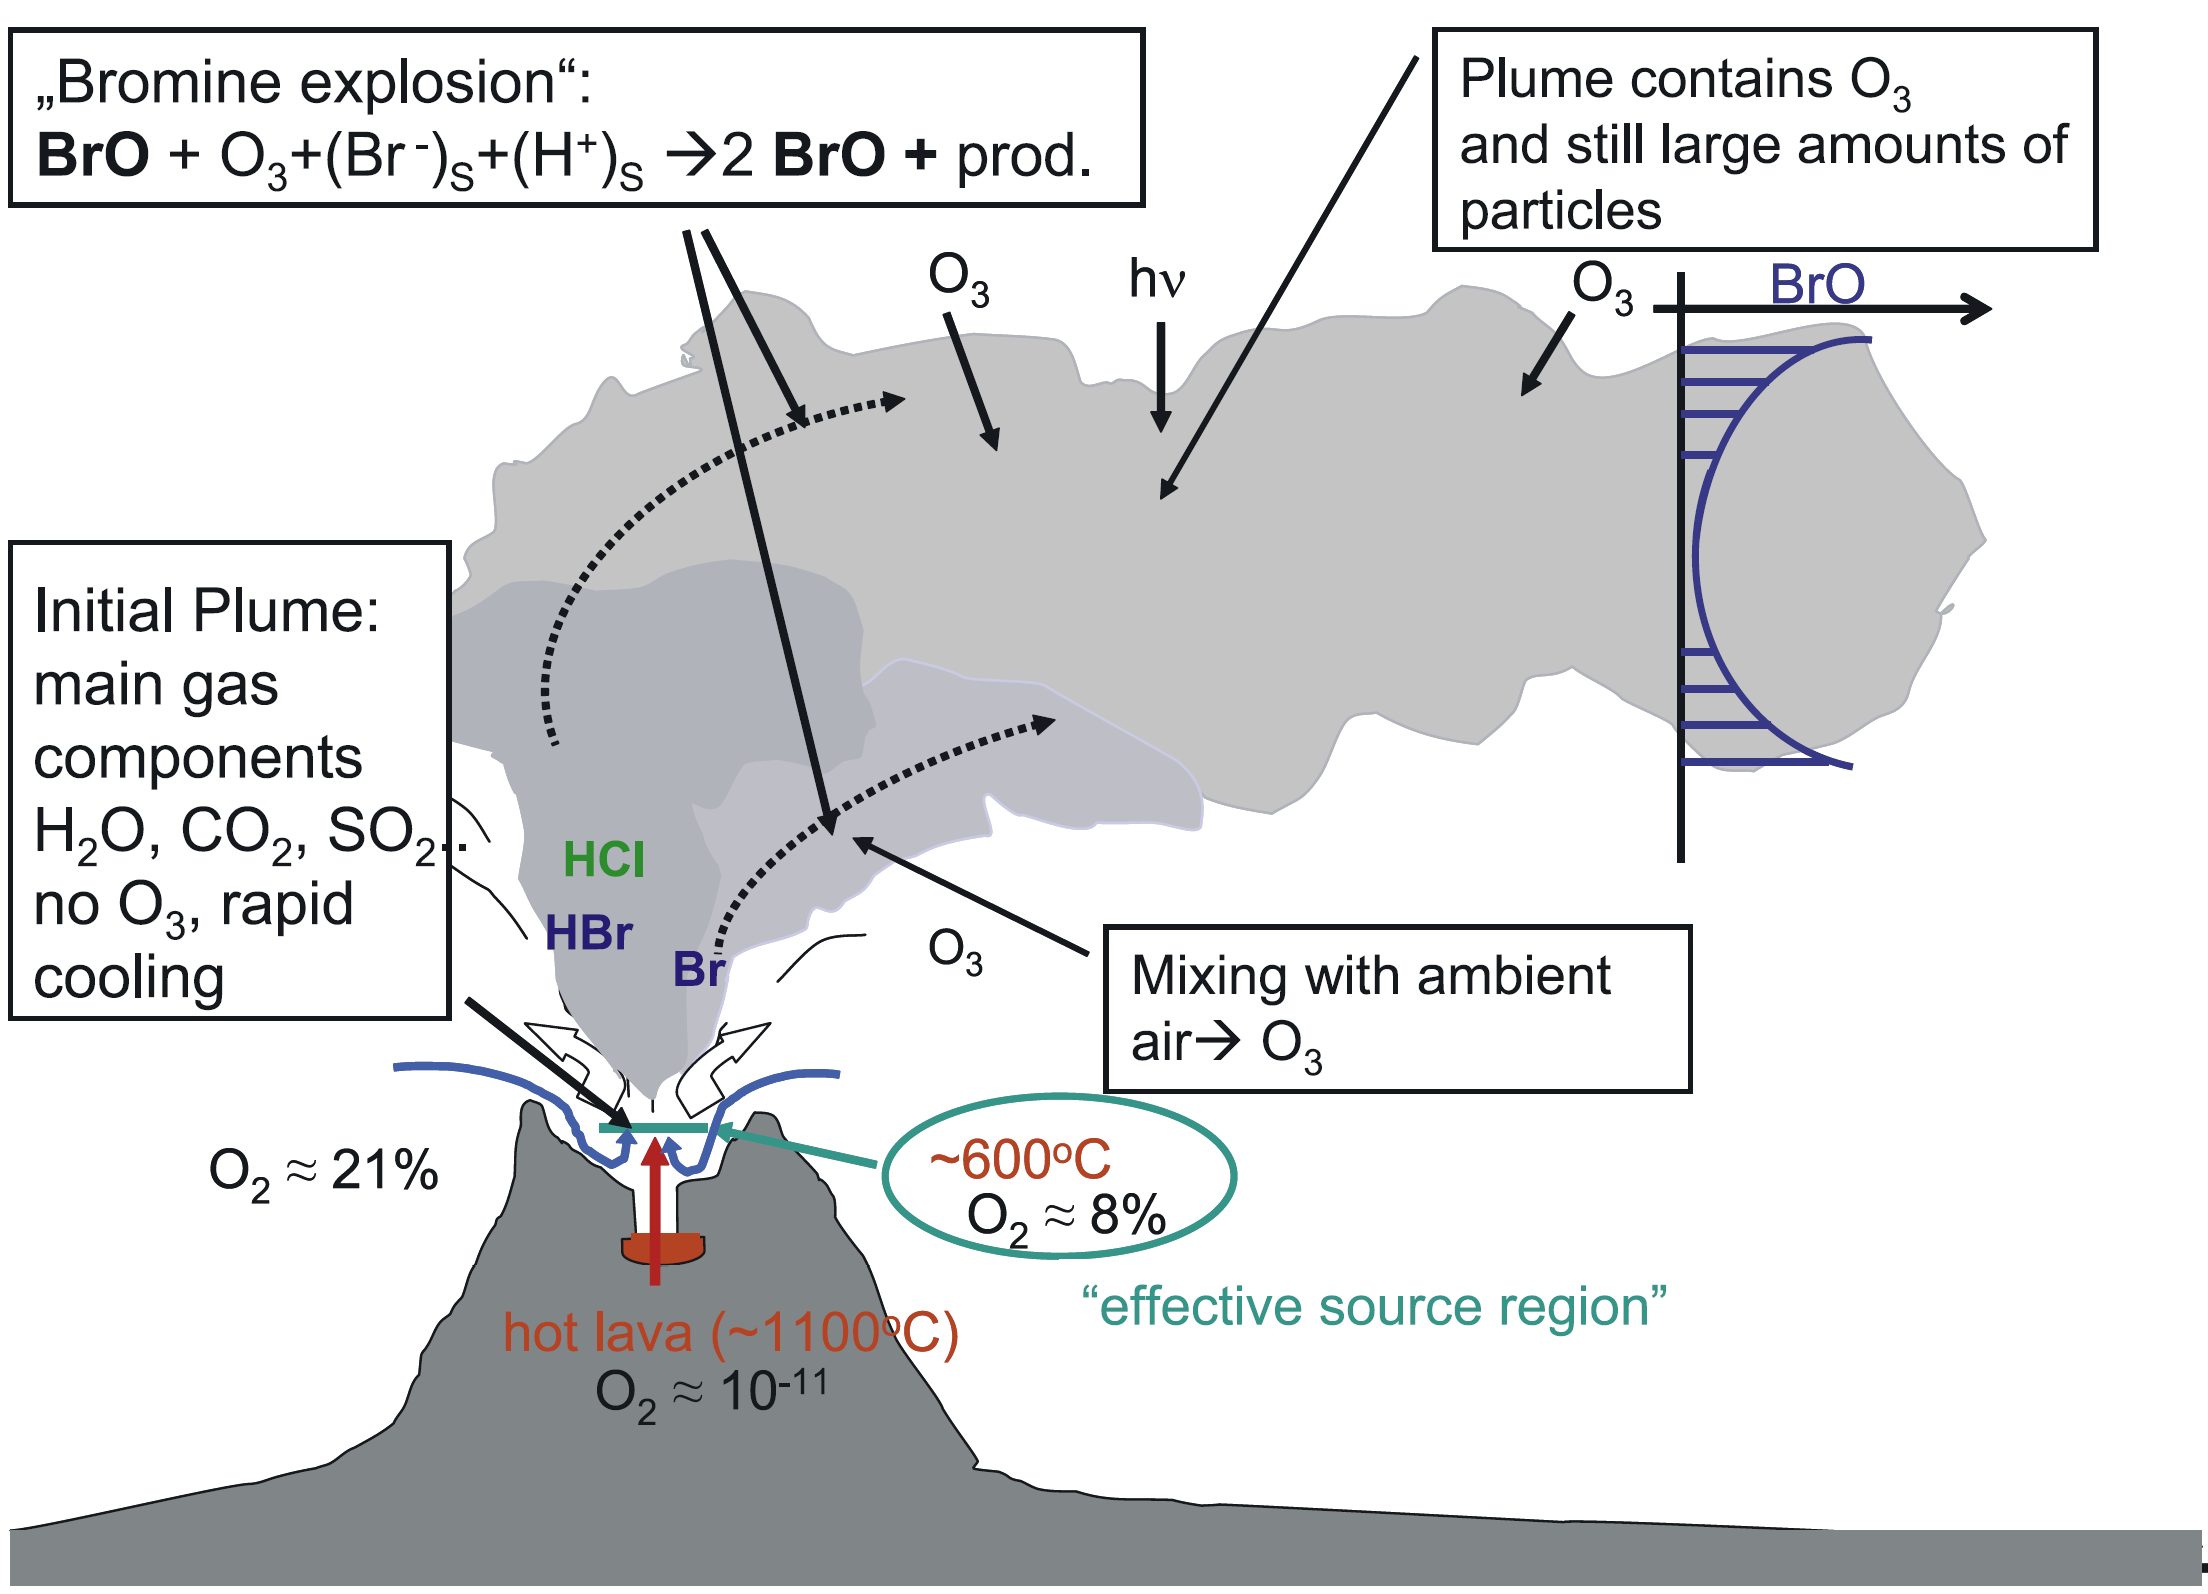
\includegraphics[width=0.7\linewidth]{Bilder/Simon/Bilder_Tung/BrO_Plume}
	\caption{schematic sketch of a Bromine Explosion.
		Release of \ce{HBr} at the volcanic vent. Mixing with ambient air in the effective source region leads to \ce{Br} formation. This resulting Bromine species react to \ce{BrO} with ozone from the plume. Adapted from \cite{bobrowski2007reactive}}
	\label{fig:broplume}
\end{figure}

\section{Volcanic plume chemistry}
\begin{figure}
	\centering
	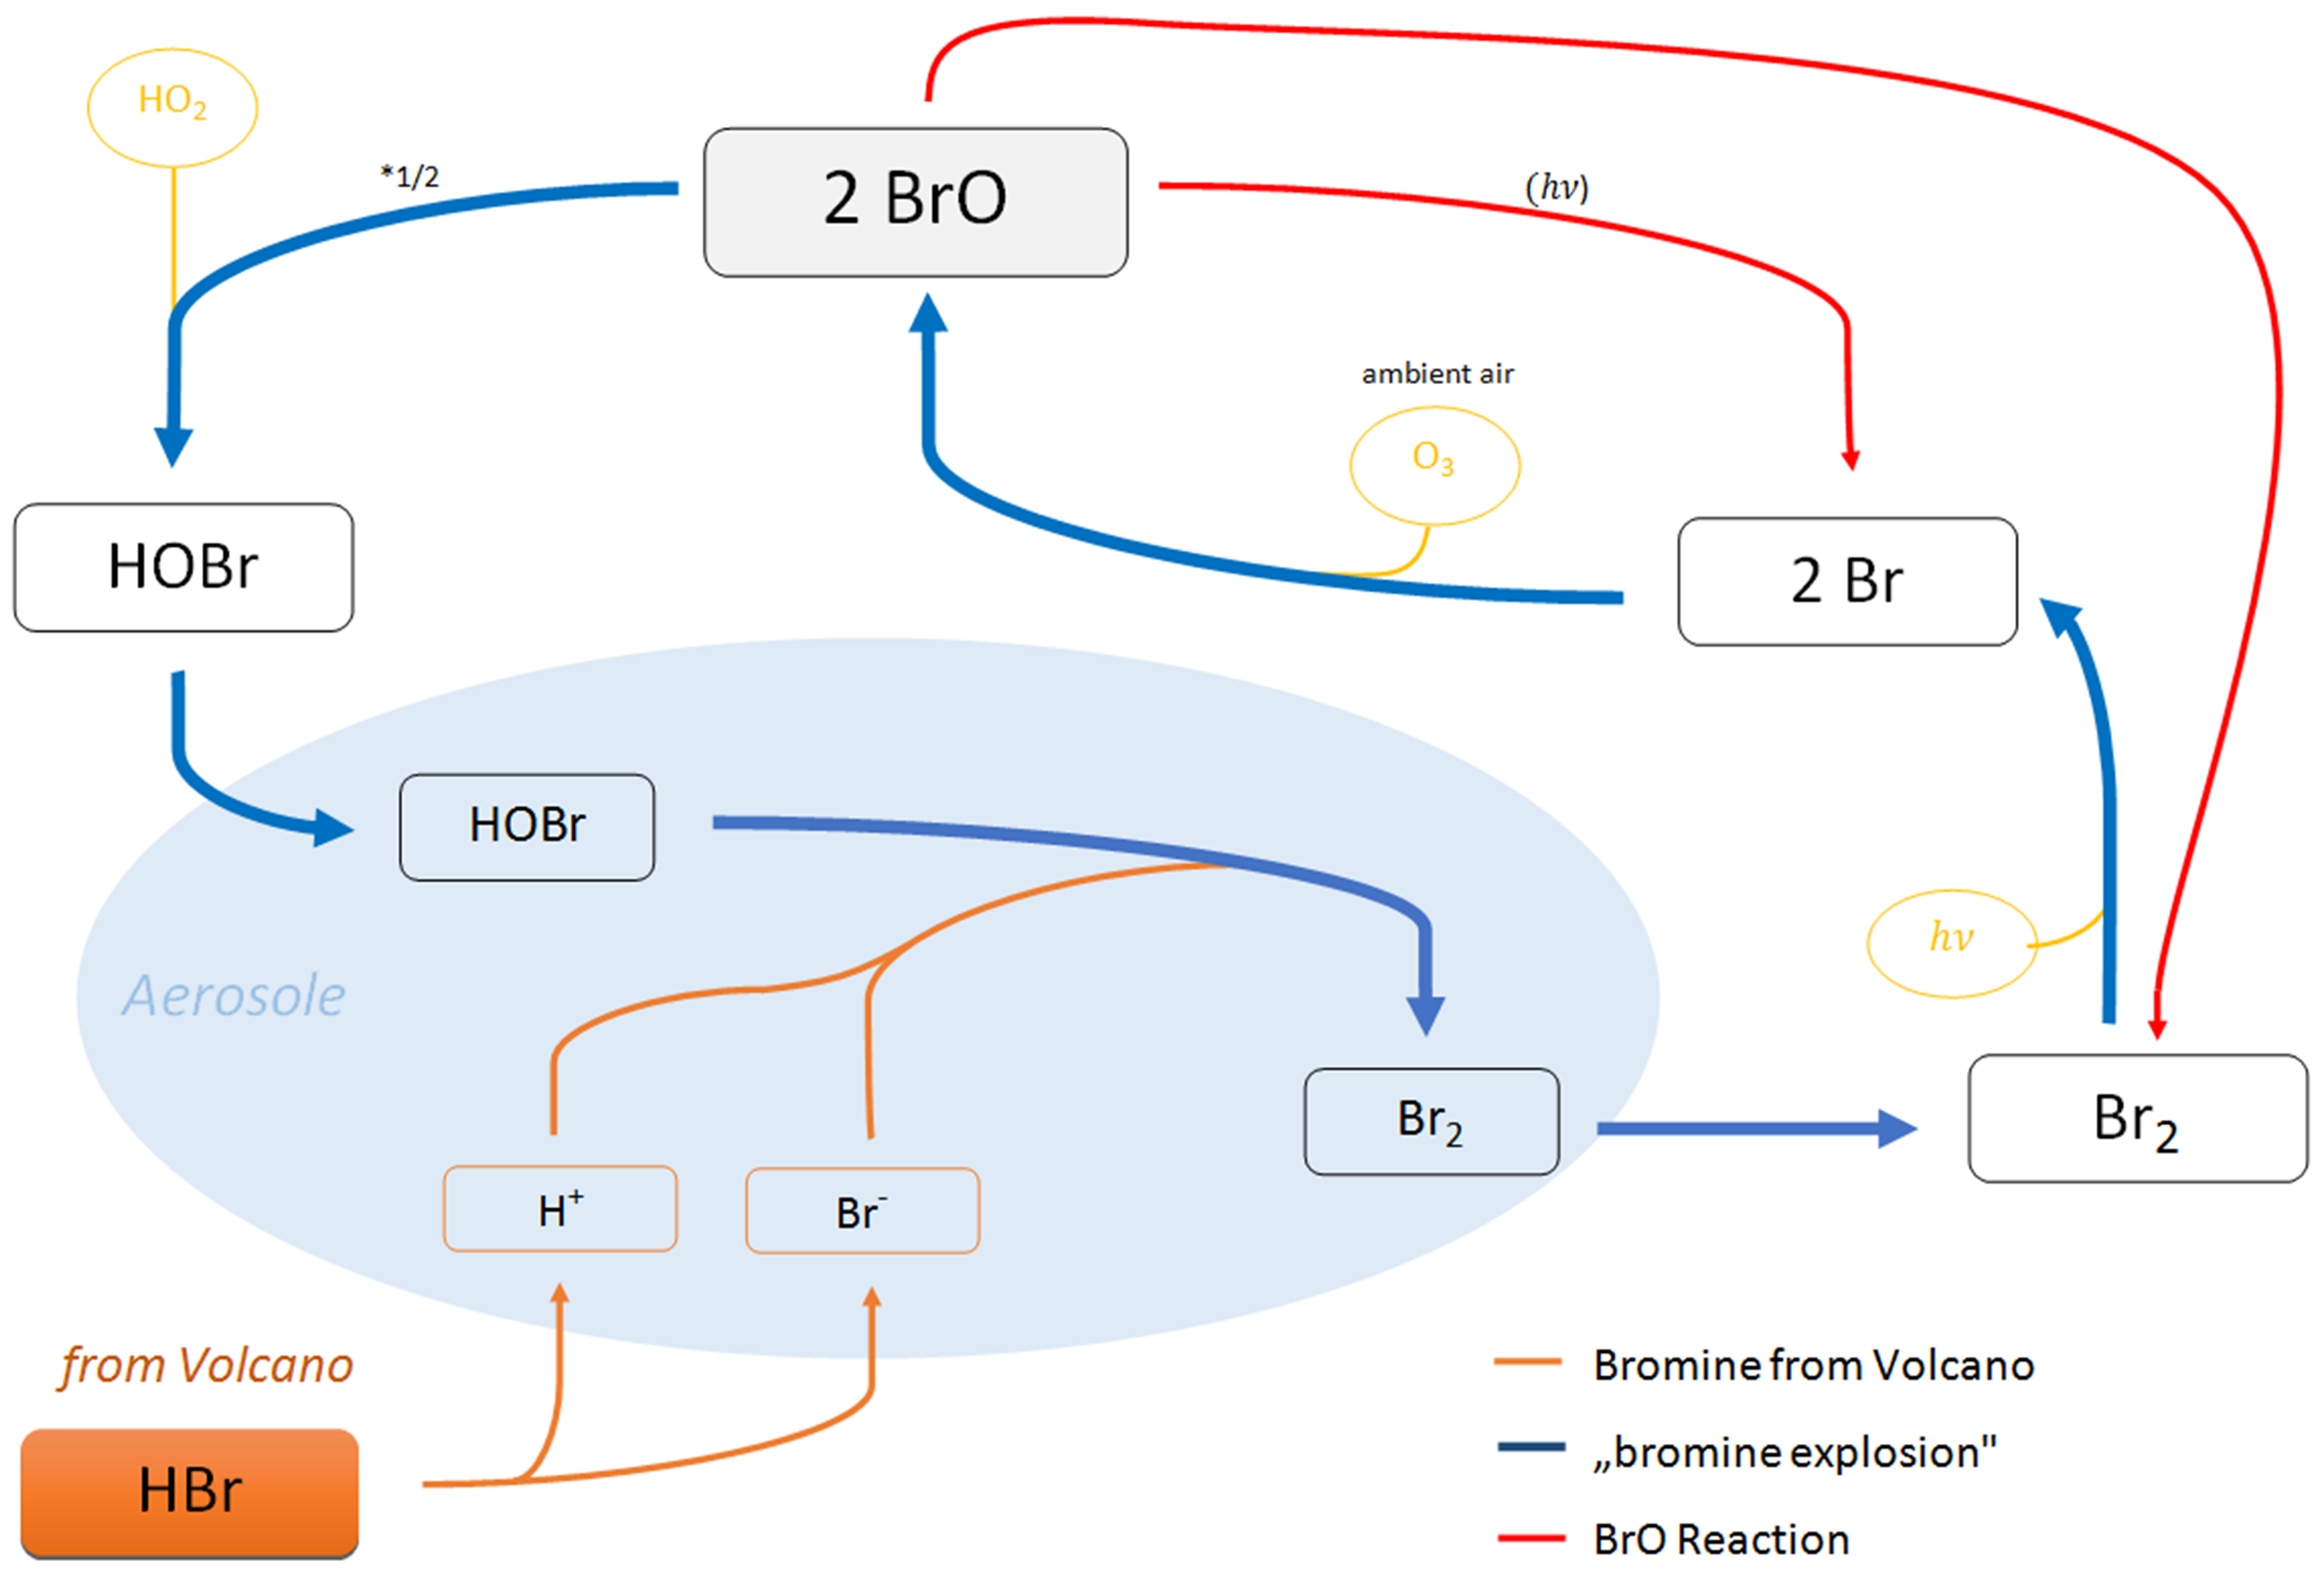
\includegraphics[width=0.7\linewidth]{Bilder/Simon/Bilder_Tung/BrO_Explosion}
	\caption{}
	\label{fig:broexplosion}
\end{figure}
\subsection{Sulphur species\label{chap:so2}}
Sulphur species are the third most abundant gases in volcanic plumes, hereby contributes SO2 with about 25\% and \ce{H2S} with 1 to 10\%. Only \ce{H2O} and \ce{CO2} have a larger share on the volcanic gases in the plume \Cref{Tab:Tracegasesinvolc}.\\
Outside of the volcanic plume the SO2 amount is with approximately 1ppb negligible, in contrast the So2 amount inside he plume can easily reach 1ppm \cite{Coppenheimer 2003}
When \ce{H2S} escapes from the volcano vent, it enters the oxidizing conditions in the atmosphere. The conversion of \ce{H2S} into \ce{SO2} starts with:
\begin{equation*}
\ce{H2O}+\ce{OH}\rightarrow \ce{H2O}+\ce{SH}
\end{equation*}
The \ce{SH} radical goes through a series of reactions, leading to the \ce{SO2} formation \cite{Seinfeld}\\
\ce{SO2} is removed from the atmosphere by dry or wet
deposition. At homogeneous reactions the lifetime is from 1-3 weeks \cite{robock2000volcanic}. Heterogenous reactions such as take place on particles or liquid phases leads to much faster depletions.\\
Further discussions of the stability of SO2 in the atmosphere can be found at \cite{lubcke2014optical}.\\
In this thesis it is assumed that SO2 is stable on timescales occurring with ground based remote sensing measuring of about 20 minutes. \\
The SO2 amount in the atmosphere outside of the volcanic plume is with approximately 1ppb negligible. In contrast the SO2 amount in the plume can easily reach 1ppm \cite{Oppenheimer}.\\
The fact that the SO2 amount in the atmospheric background compared to the SO2 amount in the plume is negligible alongside

\subsection{Bromine oxide}
The amount of Bromine in volcanic plumes is rather low compared to SO2 \cite{Bobrowski 2013}. The first time Bromine monoxid (BrO) was observed at a volcano was 2013 at the soufriere hills by \cite{Bobrowski 2013}. Since then many others were able to detect BrO using ground based remote sensing measurement techiques (DOAS: see \cref{DOAS})\\
\\
examples
\\
The main Bromine formation which is released from the volcano is  \ce{HBr}. BrO is formed due to mixing with the ozone rich atmosphere at ambient temperatures \cite{bobrowski2007reactive}.\\
Due to the raising of hot air in the volcano vent , ambient air is pulled into the vent. There temperatures of  600$^{\circ}C$ to 1200$^{\circ}C$    prevent the formation of BrO. Only Br id formed. BrO occures after further cooling and mixing while rising. When the temperature cooles down to ambient conditions the so called "Bromine Explosion" causes a non linear formation of BrO.
The "Bromine Explosion" is illustrated in \cref{fig:broexplosion} and can be described with the following reaction cycle:
\begin{align}
\ce{HBr}_{gas} &\rightarrow \ce{Br}^{-}_{aq} + \ce{H}^{+}_{aq}\\
\ce{HOBr}_{(gas)} &\rightarrow \ce{HOBr}_{(aq)} \\
\ce{HOBr}_{(aq)} + \ce{Br}^{-}_{(aq)} + \ce{H}^{-}_{(aq)} &\rightarrow
\ce{Br}_{2(aq)} +  \ce{H2O}\\
\ce{Br}_{2,aq} &\rightarrow \ce{Br}_{2,gas} \\
\ce{Br2} + h\nu &\rightarrow 2 \ce{Br} \\
\ce{Br} + \ce{O3} &\rightarrow \ce{BrO} + \ce{O2} \\
\ce{BrO} + \ce{HO2} &\rightarrow \ce{HOBr} + \ce{O2} \\
\ce{BrO} + \ce{BrO} &\rightarrow 2 \ce{Br} + \ce{O2} \\
\ce{BrO} + \ce{BrO} &\rightarrow \ce{Br2} + \ce{O2}
\end{align}

The exponential BrO formation is slightly diminished by







\section{Volcanic gases and their impact on the climate}
Volcanic gases have a large impact on the earth climate especially SO2 or more specific its oxidation product sulfur acid.\\ 
The relevance of CO2 for the climate is a subject of many discussions, the share of volcanic co2 is rather low further informations can be found in:...\\\\
\cite{halmer2002annual} estimated the mean annual SO2 emitted from volcanoes from 1972 to 200 as 7.5 to 10.5TgSyr$^-1$, while the anthropogenic So2 amount for 2000 is estimated as 55TgSyr$^-1$ \cite{IPCC}. Despite the less So2 occuring from volcanoes the impact may be higher as the impact of the antropogenic So2. \cite{graf1997volcanic} supposed that the volcaninc So2 has a higher impact on the climate since its reaches up to the stratosphere while the antropogenic so2 is mostly located in plantery boundary layer. In the lower troposhere sulphuric acid has a lifetime of about a week whereas the liftime in the stratosphere is about a year \cite{IPCC}.\\
Sulphuric acid in the atmosphere increases the aerth albedo due to direct backscattering radiation. Additional the condensation on sulphuric acid particles leads to finer droplets thus to more stable and more white clouds this increases the albedo as well \cite{twomey1974pollution}.
volcanic particles can be surfaces for heterogeneous reaction. The result is a depletion of stratospheric Ozone, and thus more high energetic solar flux on the earth surface.
Large particles may backscatter IR radiation fromt the earth surface and the lower atmosphere leading to a small reduction of the net cooling of the lower troposphere.
In the upper trophosphere ore stratosphere absorption of IR or UV radiation results in a net heating in the stratosphere and a cooling at the earth surface.
\Cref{fig:climateinfluence} shows the above described effects and their localization in the atmosphere.
The dominating radiative effect of volcanic gases is a cooling of the earth atmosphere due to  more backscattered radiation, more diffusive scattering\cite{robock2000volcanic}.
\cite{IPCC} records a volcanic radiative forcing of $-0.11Wm^{-1}$ between 2008 and 2011. For comparison the radiative of CO2 is estimated as  $1.68Wm^{-1}$.


\begin{figure}
	\centering
	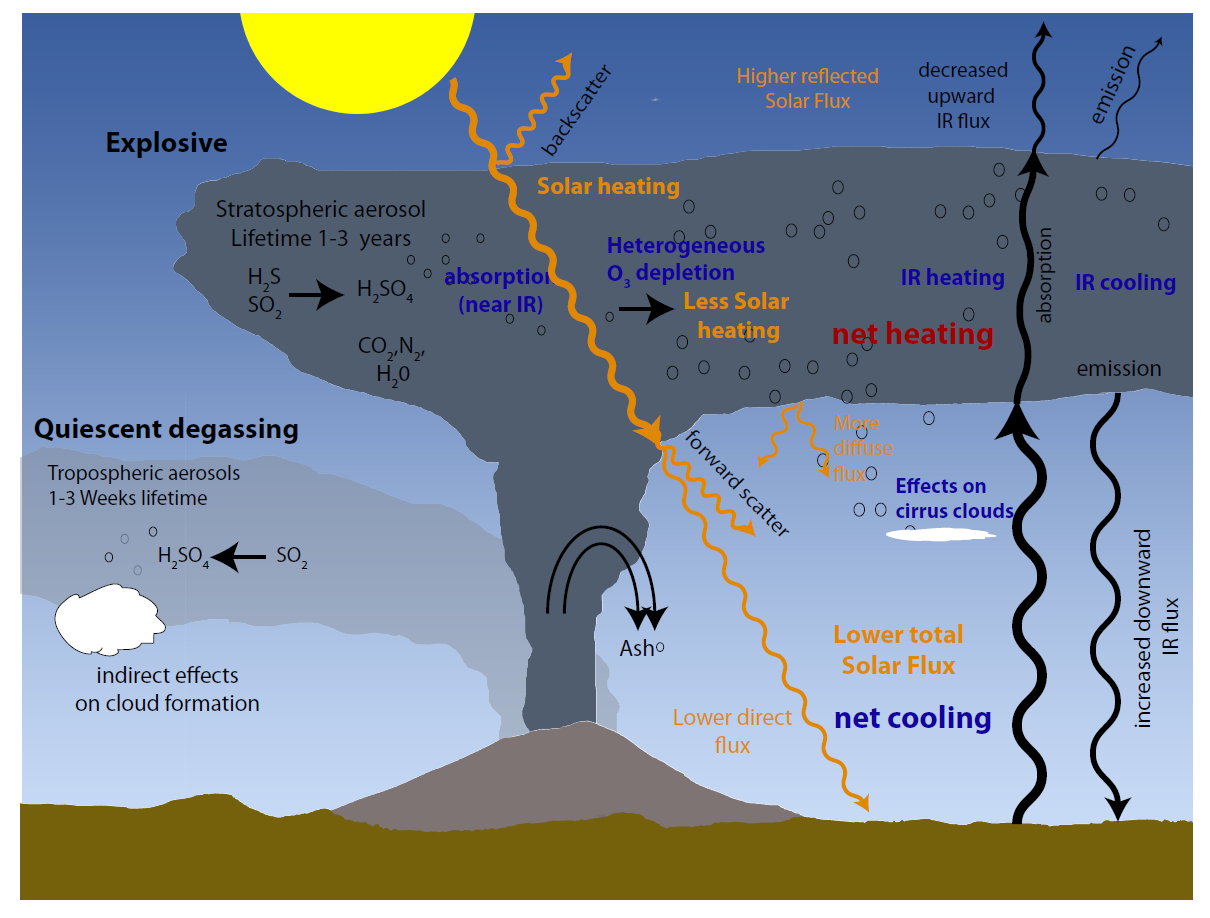
\includegraphics[width=0.7\linewidth]{Bilder/Simon/Bilder_Tung/Climate_Influence}
	\caption{Influence of volcanic eruptions and quiet degassing on earth climate. Redrawn on the basis of \cite{robock2000volcanic}}
	\label{fig:climateinfluence}
\end{figure}










\section{Using the BrO/So2 ratio to study volcanic activity}
\begin{figure}
	\centering
	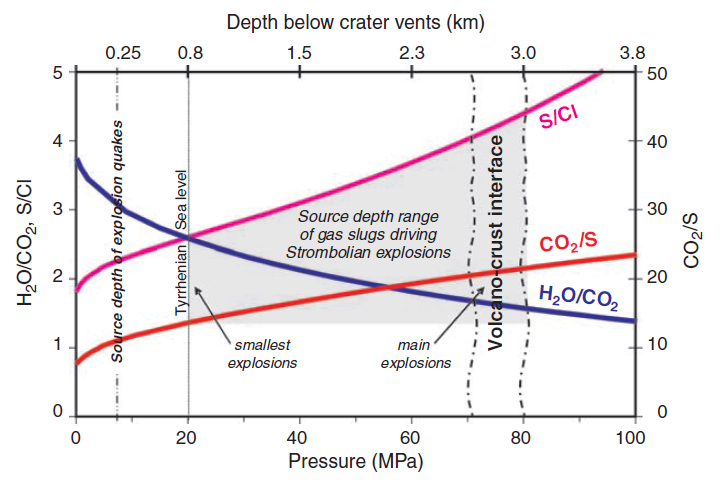
\includegraphics[width=0.7\linewidth]{Zwischenbericht2018/Bilder/so2_bro}
	\caption{Dependency of the ratios of different volcanic trace gases on depth. Data originate from Stromboli volcano. From \cite{lubcke2014optical} reproduced from Burton et al. (2007)}
	\label{fig:so2bro}
\end{figure}    
	
	Volcanic degassing is influenced by many factors, which can be exploit to study volcanic activity by using the gas composition of the volcano plume. Therefore remote sensing should be an additional tool for forecasting of volcanic activity next to classical monitoring techniques like seismographic and deformation measurements.\\
	Inside of volcanoes volatiles are in solution in magmatic melt. The Henry law \cref{Henrylaw} describes the necessary conditions for gas formation:
	\begin{equation}
	P = K_{H}\cdot c
	\label{Henrylaw}
	\end{equation}
	Here P is the partial pressure at equilibrium of the solute, c is the concentration and $ K_{H}$ is the Henry constant which is anti proportional the the solubility $\alpha$ ($\alpha = \frac{1}{ K_{H}}$).
	If the partial pressure of the gas solute (in this case a magmatic gas constituent) exceeds the pressure of the surrounding solvent, a formation of gaseous bubbles occur. Otherwise, if the partial pressure of the gas in the solution is below the surrounding pressure the formation of gas bubbles stops.\\
	The solubility $\alpha$ depends on the temperature, the chemical composition and on the solvent (here magma). Whereas the partial pressure of the constituent depends on the surrounding pressure. The pressure below the volcanic vent increases with depth, this leads to a correlation between the partial pressure of the constituents and the depth.
	The result is, that the gas starts exsolving at a certain depth depending on the  partial pressure of the constituent. Thus the gas bubble formation increases with rising magma. But at a certain depth the percentage of solved gas is different for each volcanic gas. The result is, that the composition of the gases changes with depth. So gas ratios contain information about its originating source depth.\\
	Prior to volcanic eruptions the magma starts raising since the gas is mostly less dense than the magma it raises faster and could be therefore a indicator for its origin source depth thus a indicator for the volcanic activity.\\
	\Cref{fig:so2bro} shows the ratios of H2O/CO2,S/CL,CO2/S as a function of the pressure respectively on the depth. 
	%
	Especially halogen-sulfur ineresting due to ambient air concentrations are negligible
	%
	Noguchi and kamiya 1963 found decrease Cl/S prior to eruptive periods
	%
	pennisi and le cloarec 1998 lower CL/S ratio during reuptive periods than not erutive periods at etna
	%
	Burton et al 2007 at stromboli co2/so2 so2/hCl ratios 3-5 times higher during explosions  compaered to quiet degasing
	%
	the authors compared these data to gas formation simulations for different degassing source depth (see fig ..) they concluded that these eruptions were driven by gas slugs from deeper levels where the ratios were higher while quiet degasing originates from from shallow magma
	%
	BrO/SO2 curves like in fig .. are not avalible due to lack of  bromine solubility curve but the following observations were made:
	%
	changes of BrO/So2 were found by bobrowsky and giuffrida 2012: multiple eruptions between 2006 and 2009 highest ratios 2-3 month before the eruptions the ratio then decreased and was lowest during eruptiv ephase -> bromine exsolved ealyer at lower depth than sulphur 
	%
	lübke found decrease of bro 5 month prior to th eruption 2012 at nevado del ruiz can also be atributed to a earlyer exsolution of bromine during rising magma
	%
	Despite the lack of the solubility curve of BrO until now, the BrO/SO2 has a great potential for investigations of the volcanic activity. The first reason is, that both gases can be measured with remote sensing by DOAS instruments. For examples ground based measurements by \cite{bobrowski2007reactive},\cite{lubcke2014optical} ore satelite based measurement by \cite{Hörman et al 2013}ore \cite{Beirle at al 2014}. The advanteg of remote sensing techniques is the possibility of measuring during eruptions which is with in situ measurements not always possible.
	Secondly due to the NOVAC network (See \ref{NOVAC}) continues measurements are possible.\\
	Another reason for the research on BrO/SO2 ratios at volcanoes is the constance of the ratio from 5 to at least 30 minutes after release \cite{bobrowski2007reactive};\cite{lubcke2014optical}. As well as the constance from 5 to 20 km off the volcano see \ref{bild von Simon noch kriegen}. This ensures that the data measured from different positions or at different conditions are comparable.\\
	\\
	This chapter motivated the research on the BrO/SO2 ratio as a tracer for volcanic activity.
	
	
	
	
	
	
	
	
	
	
	
	
	
	

	\subsection*{Tungurahua}
	Tungurahua is a subduction zone volcano located in the Ecuadorian Andes (Lat: 01$^{\circ}$,28$^{'}$S; Long:78$^{\circ}$,27$^{'}$W). 2014 Tungurahua was one of the most active volcanoes in southern America, since then the activity was decreasing. Tungurahua is 5023m high and is one of the defining volcanoes of the eastern volcanic rows in Ecuador. \cite{hall1999tungurahua}\\
	Welche daten von welchen zeiten werden angeschaut??\\
	In welcher groeßenordnung sind die gasaustritte in der beochteten Zeit?
		
	\subsection*{Nevado Del Ruiz}
	Nevado Del Ruiz is also a subduction zone volcano. 	Nevado Del Ruiz  is located in the Central Cordillera of Colombia, 140 km west of Bogota.
	(Lat: 04$^{\circ}$,53$^{'}$S; Long:75$^{\circ}$,19$^{'}$W) 
	The hight of Nevado Del Ruiz is 5389 m.
	\\
	Welche daten von welchen zeiten werden angeschaut??\\
	In welcher groeßenordnung sind die gasaustritte in der beochteten Zeit?
	 
	\chapter{Remote sensing of volcanic gases}
	In this thesis we are interested in the volcanic trace gases \ce{SO2} and BrO, both measured with the Differential Optical Absorption Spectroscopy (DOAS) a remote sensing technique proposed by \cite{platt2008differential}\\
	

	\section*{Beer-Lambert Law}
	The Lambert-Beer law describes the attenuation of light when traveling through a material.\\
	This section will give an overview about the reasons for decreasing light intensity when going through a medium.\\
	The Lambert-Beer law describes the attenuation of light when traveling through a material.\\
                                                                                                                                                                                                                                                                                       ,
	Atoms and Molecules exists in several energy states, depending on the different electron configuration. Moreover Molecules have additionally rotation and vibration states, also enclose to the energy states. If a photon matches the energy gap between two possible energy states, this includes, that the lower energy state is occupied and the selection rules are fulfilled  the molecule could absorb the photon, remaining in a higher energy state.\\
	The additional photon energy could be loosed by collision with another molecule or by emission. But since the direction of the emitted photon is mostly not the same direction of the absorbed photon the intensity I$_{0}$ of the light before passing the medium is higher than the intensity I after traveling the distance L through the medium.\\
	This can be described as:\\ 
	\begin{equation}
	I\left(L,\lambda\right) = I_{0}\left(\lambda\right)\cdot expt\left(-\int^{L}_{0}\sigma\left(\lambda,p,T\right)\cdot c\left(l\right)dl\right)
	\end{equation}
	where $c\left(l\right)$ is the location-dependent concentration of the trace gas of interest. $\sigma\left(\lambda,p,T\right)$ is the absorption cross section, $\sigma\left(\lambda,p,T\right)$ is unique for each molecule and depends on pressure p and on the temperature T.\\
	%
	An important quantity used in many optical remote sensing techniques is the optical density $\tau$. The optical density is a measure for the weakening of radiation when going through a material. $\tau$ can be calculated using the lambert beer law:
	\begin{equation}
	\tau = -ln\left(\frac{I\left(\lambda\right)}{I_{0}\left(\lambda\right)}\right) = \sigma\cdot S
	\end{equation}
	Hereby is $S$ the column density. The column density is the concentration of the trace when integrating along the light path, the dimension of $S$ is therefore the number of molecules divided by an area: $\frac{molec}{cm^2}$.
	\begin{equation}
	S = \int_{0}^{L}c\left(l\right)dl
	\end{equation}
	%
	When measuring at a volcano, that means measuring in the atmosphere the situations gets more complex, since we need to deal with several absorbers and scattering processes have to be taken into account. One possibility is to treat scattering effects as pseudo absorbers with the respective extinction coefficients for Rayleigh ($\epsilon_R$) and  Mie ($\epsilon_M$) scattering
	\begin{equation}
	I\left(L,\lambda\right) = I_{0}\left(\lambda\right)\cdot expt\left(-\int^{L}_{0}\sum_{j}\sigma_{j}\left(\lambda,p,T\right)\cdot
	c_{j}\left(l\right)+\epsilon_R\left(\lambda,l\right)+\epsilon_{M}\left(\lambda,l\right)dl\right)
	\label{eq:lbe}
	\end{equation}
	The first term of \cref{eq:lbe} in the exponential function, multiple absorbers $j$ are considered, the corresponding concentration depends on the position l of the light path.
	The last two terms in describe the extinction due to Rayleigh and Mie scattering in the atmosphere.\\
	Inelastic scattering (for example the Ring effect) and effects due to turbulences in the atmosphere are neglected here.

	\section{Differential Optical Absorption Spectroscopy(DOAS)\label{DOAS}}
		\begin{figure}
			\centering
			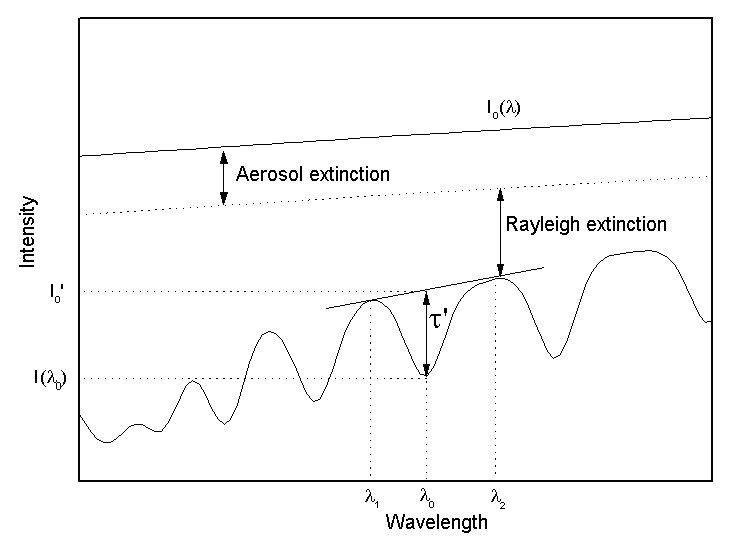
\includegraphics[width=0.7\linewidth]{Bilder/Simon/Bilder_Tung/DOAS_Intensity}
			\caption{Basic idea of the DOAS principle: Light attenuate due to broad band and narrow band effects. The broad band extinction is caused by aerosols and Raylight scattering $\left(I_0\rightarrow I^{'}\right)$. The measured intensity $I$ is formed by narrow band effects due to differential absorption structures by trace gases with the optical density $\tau^{'}$. Adapted from \cite{kern2009spectroscopic}}
			\label{fig:doasintensity}
		\end{figure}
		
	It is impossible to distinguish between various broad-band effects, like scattering in the atmosphere or instrument effects which influence the measured spectra \cite{lubcke2014optical}. Therefore \cref{eq:lbe} cannot be applied to real measurements.\\
	Differential Optical Absorption Spectroscopy (DOAS) was invented in the late 1970s by \cite{perner1979detection}. This section will give an overview about the DOAS technique. More detailed information ca be found in the work of \cite{platt2008differential}\\
	\newline
	Differential Optical Absorption Spectroscopy uses the fact, that absorption can be divided into broad-band parts and narrow-band parts. Broad band parts are effects that only changes weakly with the wavelength,  i.e. scattering and instruments effects have a broad-band structure. 
	The narrow band part includes effects that strongly depends on the wavelength.
	Within the DOAS-Method only narrow-band absorption features of molecules are used to obtain their column densities.
	The absorption cross section of trace gases $j$ have broad-band ($\sigma_b\left(\lambda \right)$) and narrow band ($\sigma{'}\left(\lambda \right)$) features, only the narrow-band structures are used in DOAS.
	\begin{equation}
	\sigma\left(\lambda \right) = \sigma_b\left(\lambda \right) + \sigma{'}\left(\lambda \right)
	\end{equation}
	%
	With this considerations the Lambert-Beer law \cref{eq:lbe} can be rewritten
	dividing the exponential part into a narrow-band part and a broad-band part:

	\begin{align}
	I\left(\lambda,L\right) = &\overbrace{I_{0}\left(\lambda\right)\cdot exp\left(-\int^{L}_{0}\sum_{j}\sigma_{b,j}\left(\lambda,p,T\right)\cdot c_{j}\left(l\right)+\epsilon_R\left(\lambda,l\right)+\epsilon_{M}\left(\lambda,l\right)dl\right)}^{=I^{'}_0\left(\lambda\right)} \cdot \nonumber \\
	&exp\left(-\int^{L}_{0}\sum_{j}\sigma_{j}^{'}\left(\lambda,p,T\right)\cdot c_{j}\left(l\right)dl\right)
	\label{eq:bb}
	\end{align}	
		%
	The so defined $I^{'}_0\left(\lambda\right)$ differs from $I_0\left(\lambda\right)$ only by broad band effects. With $I^{'}_0\left(\lambda\right)$ a differential optical density $\tau^{'}$ can be defined:
	\begin{equation}
	\tau^{'} = ln\left(\frac{I^{'}_0\left(\lambda\right)}{I\left(\lambda\right)}\right) = \int_{0}^{L} \sum_{j} \sigma^{'}_{j} \cdot \left(\lambda\right) \cdot c_{j}\left(l\right)dl = \sum_{j}\sigma^{'}_{j}\left(\lambda\right)\cdot S_{j}
	\label{eq:taustrich}
	\end{equation}
	
	The optical density can now be calculated by using the difference of the column density $S_{M}$ in the measurement spectrum to the column density $S_{R}$ of a reference spectrum. From \Cref{eq:bb} we know:	
	\begin{equation}
	I_{P,R} = I^{'}_{0}\cdot exp\left(-S_{P,R}\cdot\sigma\left(\lambda\right)\right)
	\label{eq:smr}
	\end{equation}
	In general the obtained column density $S_{M}$ is called differential slant column density: "dSCD". If the reference spectrum does not contain the trace gas of interest (is not contaminated with trace gases) that means $S_{R} = 0$, $S_{M}$ is called the slant column	density (SCD). 
	With \Cref{eq:smr} the optical density can be derived by:
	\begin{equation}
	\tau\left(\lambda\right) = -ln\left(\frac{I_{M}}{I_{R}}\right) = \sigma\left(\lambda\right)\cdot\left(S_{M}-S_{R}\right)
	\end{equation}
	%

	
	
	\subsection{Technical Implementation of the DOAS Approach}
	The theory explained above only describes the ideally situation. In real measurements more problems occur due to instrument limitations inelastic scattering causing the Ring effect and due to impacts of external parameters like temperature.\\
	In the following a short overview about these problems and their consequences for our retrieval is given. Further information can be found in \cite{lubcke2014optical}.\\
	\subsubsection*{Optical and spectral resolution of the spectrometer}
	The resolution of the spectrometer is finite, thus, the detector receives a spectrum $I^{*}\left(\lambda\right)$ which can be retrieved with a convolution of the incident spectrum $I\left(\lambda\right)$ with the instrument function H$\left(\lambda\right)$:
	\begin{equation}
	I^{*}\left(\lambda\right) = I\left(\lambda\right)*H\left(\lambda\right)=\int I\left(\lambda-\lambda{'}\right)\cdot H\left(\lambda-\lambda{'}\right)d\lambda{'}
	\end{equation} 
	For the evaluation all $\sigma_{j}$  of the trace gases of interest need to have the same spectral resolution as the instrument used for recording the spectra. In this work we will use high resolution cross sections and convolute them with the instrument function H:
	\begin{equation}
	\sigma{*}\left(\lambda\right) = \sigma\left(\lambda\right)*H\left(\lambda\right)
	\end{equation}
	The instrument function H can be approximated by using a the spectral lines of an mercury lamp since the width of those lines is only a few pm, they could be treated as delta peaks when comparing it to the resolution of the spectrometers.
	
	\subsubsection*{Effects of the detector}
	The detector only has discrete pixels, therefore a wavelength interval is mapped to a pixel $i$.
	
	\begin{equation}
	I^{'}\left(i\right) = \int_{\lambda(i)}^{\lambda(i+1)}I^{*}\left(\lambda{'}d\right)d\lambda{'}
	\end{equation}
	For the retrieval the relationship between the detector channels and the wavelength of the spectrum need to be known.
	The wavelength to pixel mapping (WMP) for a detector with q channels can be calculated as:

	\begin{eqnarray}
	\lambda(i) = \sum_{k=0}^{q-1}\gamma_{k}\cdot i^{k}
	\end{eqnarray}
	Hereby, is $\gamma_{0}$ a shift of the spectrum and $\gamma_{1}$ is a squeeze (respectively stretch) of the spectrum.
	The wavelength to pixel mapping can be discovered by using a mercury lamp again and compare pixel-position with the well known wavelength of the individual HG-lines of the mercury lamp.\\
	The wavelength to pixel mapping depends on the instrument temperature as well as on the ambient pressure \cite{lubcke2014bro}.
	\subsubsection*{Ring effect}
	As mentioned above inelastic scattering causes the Ring effect (named after Grainger and Ring, 1962).
	The Ring effect is observable through a filling of the Fraunehofer lines in spectra of scattered solar radiation, (e.g. if the sunlight travels through the earth atmosphere). When compared to direct sunlight measurements (e.g. outside of the earth atmosphere).
	(\cite{bussemer1993ring},\cite{solomon1987interpretation}) proposes that the Ring effect is a result of  rotational Raman scattering mainly of
	$O_2$ and $N_2$ in the atmosphere.
	\cite{solomon1987interpretation} suggested to treat the Ring effect as a pseudo-absorber. 


	
	\part{Evaluation of the Data of Tungurahua and Nevado Del Ruiz}
	
	
	\chapter{Network for Observation of Volcanic and Atmospheric Change \label{NOVAC}}
	%	
	

%% NOVAC
%% =============
%%
		\begin{figure}[h]
			\centering
			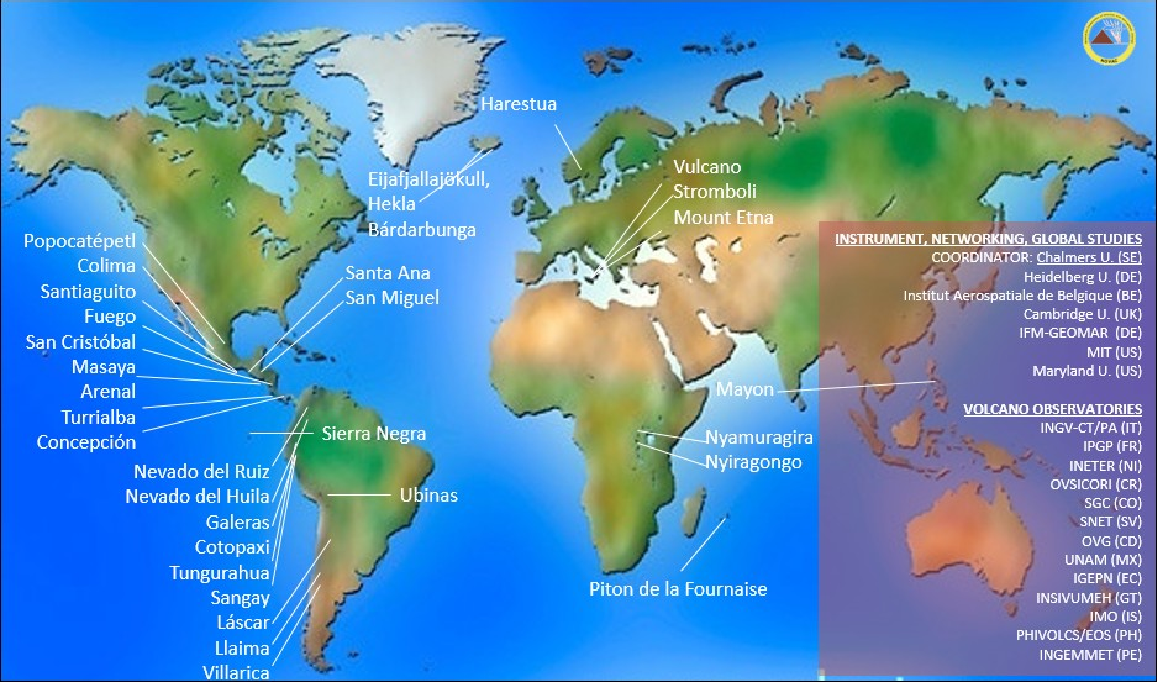
\includegraphics[width=0.8\linewidth]{Bilder/NOVAC2015}
			\caption{Global map of the volcanoes monitored by NOVAC. Used with friendly permission of Santiago Arellano.}
			\label{fig:novac2015}
		\end{figure}
		Network for Observation of Volcanic and Atmospheric Change (NOVAC) is a network of instruments monitoring volcanoes over the whole world. 
		%
		The aim of NOVAC is to gain another tool for risk assessment, for gas emissions and geophysical researches. Also many other scientific purposes are build on the data from NOVAC.\\
		%
		NOVAC was originally funded by the European Union on the first October in 2005. The aim of NOVAC is to  establish  a  global  
		network  of  stations  for  the  quantitative  measurement  of  volcanic gas  emissions. At the beginning, NOVAC encompassed observatories of 15 volcanoes in Africa America and Europe, including some of the most active and strongest degassing volcanoes in the world. Although the EU-funding has stopped, the network has been constantly growing since it was founded. In 2017 more than 80 Instruments are installed at over 30 volcanoes in more than 13 countries.
		\Cref{fig:novac2015} shows a map, with all volcanoes of the Network for Observation of Volcanic and Atmospheric Change.\\
		
		The great advantage of the data monitored in NOVAC is the fact
		that NOVAC provides continues gas emission data over many years. This ensures statistically meaningful results for the data evaluation.\\
		The instruments used in NOVAC are scanning UV-spectrometer named Mini Doas instruments. \\
		The  Mini DOAS  instrument  represents  a  major  breakthrough  in  volcanic  gas	monitoring as it is capable of real-time semi-continuous unattended measurement of the total emission fluxes of  \ce{SO2} and BrO from a volcano. Semi-continues in this case means that the measurement is only possible during daytime when enough Sunlight is there.\\
		%
		\begin{figure}
			\subfigure[Bezeichnung der linken Grafik]{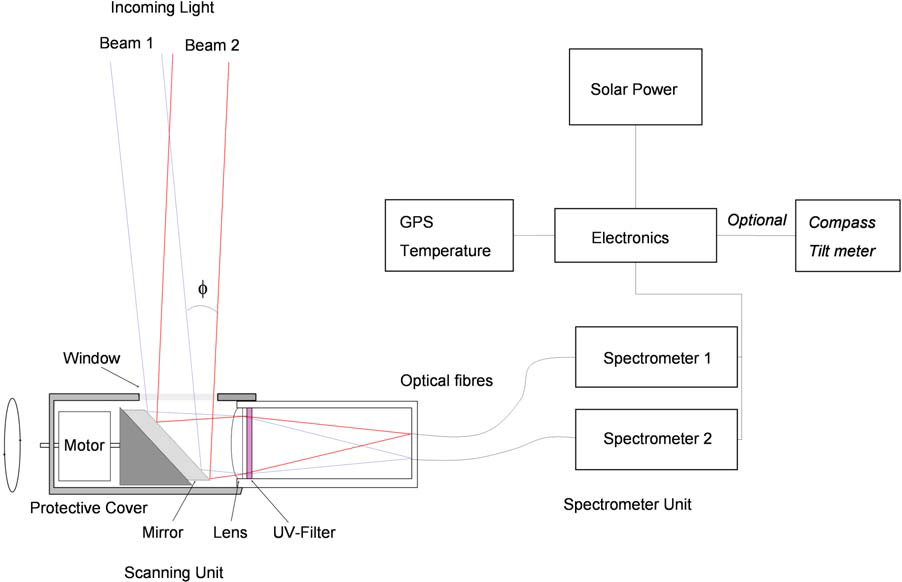
\includegraphics[width=0.49\textwidth]{Bilder/Simon/Bilder_Tung/NOVAC_Instrument}}
			\subfigure[Bezeichnung der rechten Grafik]{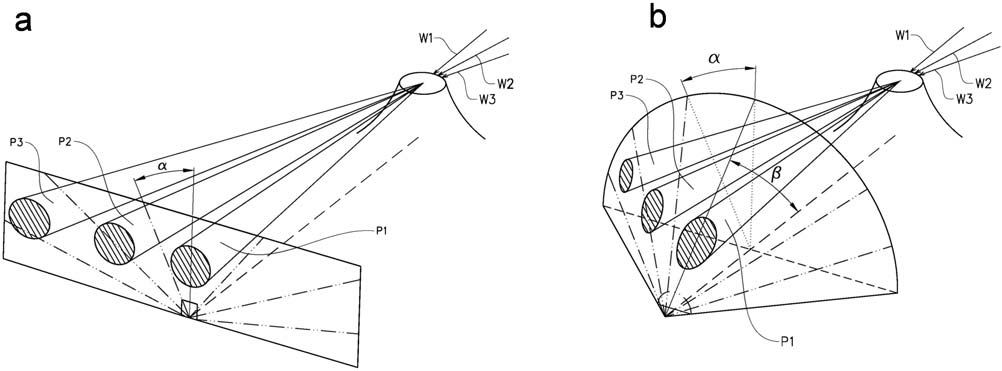
\includegraphics[width=0.49\textwidth]{Bilder/Simon/Bilder_Tung/NOVAC_scan_geo}}
			\caption{Titel unterm gesamten Bild}
		\end{figure}
		The  basic  Mini DOAS  system  consists  of  a  pointing  telescope  fiber-coupled  to  a  spectrograph.  
		Ultraviolet light from the sun, scattered from aerosols and molecules in the atmosphere, is collected by 
		means  of  a  telescope  with  a  quartz  lens  defining  a  field-of-view  of  12~mrad.
		\cite{NOVACsite} \\
		The spectrometers measure in the UV region in a wavelength range of 280 to 420~nm. In this range the differential structures of \ce{SO2} and BrO are dominant.
		\\
		The NOVAC-instruments need to be very robust to stand the conditions around volcanoes. Therefore the design of the instruments is rather simple, this means the instruments do not have internal stabilisation features like temperature stabilization to keep the measurement independent of external parameters.\\
		This comes with a reduced precision of the data, but the huge amount of data produced by NOVAC compensates for this limitation.  
		
		
		\section{Measurement Routine}
		\begin{figure}[h]
			\centering
			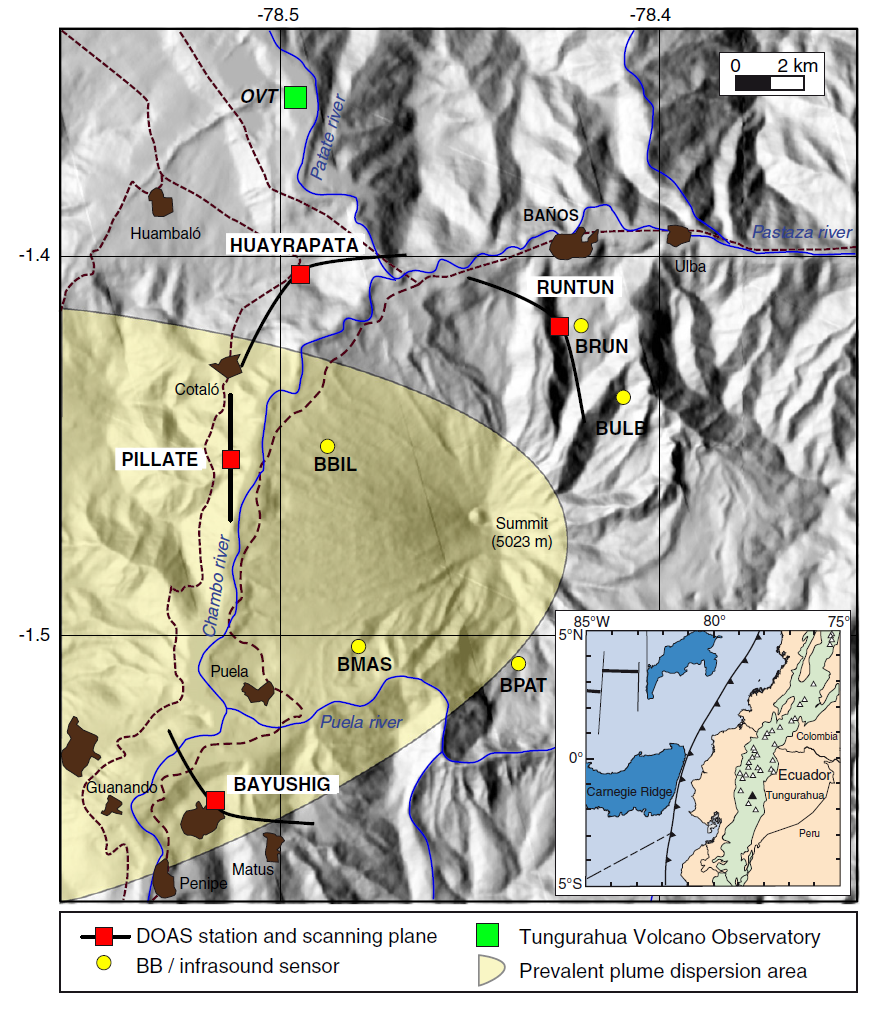
\includegraphics[width=0.6\linewidth]{Bilder/Simon/Bilder_Tung/Map_Tungurahua2}
			\caption{}
			\label{fig:maptungurahua2}
		\end{figure}
		The Instruments are set up five to ten km downwind of the volcano. To cover most of the occurring wind directions two to five instruments are installed at each volcano. Ideally, the measurement plane is orthogonal to the plume, to get the best measurement results. In reality, the measurement plane might be rotated.\\
		The Instruments record spectra in different viewing angles covering a the hole sky from horizon to horizon.\\
		The zenith is at 0$^{\circ}$.
		The measurement routine starts with a spectrum in zenith direction: the pre-reference.
		Afterwards, the dark current spectrum is recorded.\\
		Then the Instrument turns automatically to the side, recording spectra at the elevation angle from -90$^{\circ}$ to 90$^{\circ}$ with steps of 3.6$^{\circ}$. \\
		One hole measurement takes 6 to 15 minutes.
	
	\chapter{Evaluation Routine}
		This chapter will go through the algorithm which is used for the evaluation of the spectroscopic data recorded in NOVAC. 
		The occurring problem of contamination of the reference will be explained and possible solutions will be presented.
		 
	\section{NOVAC-Evaluation}
		The fitting routine used for this thesis is based on the DOASIS software \cite{kraus2006doasis}. 
		The equations of the DOAS retrieval of this work are slightly different from \cref{eq:taustrich}.
		\Cref{eq:lbe} can be rewritten to:
		\begin{align}
		ln\left(I\left(\lambda, L\right)\right) = &ln\left(I_0 \right) + P \left(\lambda\right) -	\int_{0}^{L}\sum_{j}\sigma_j \left(\lambda, p, T \right) \cdot c_j \left(l\right)dl \nonumber \\
		= &ln\left(I_0 \right) + P \left(\lambda\right)-
		\sum_{j}\sigma_j \left(\lambda, p, T \right) \cdot S_j
		\label{eq:lben}
		\end{align}
		%
		The term $ P \left(\lambda\right)$ is a polynomial that accounts for all broad-band effects that differ between the background spectrum $I_0\left(\lambda\right)$ and the measurement spectrum $I\left(\lambda\right)$.\\

		The remaining task of the DOAS routing is to find a model function $F \left(\lambda\right)$ that minimizes $\chi^2$:
		\begin{equation}
		\chi^2 = \sum_{i=\lambda_1}^{\lambda_2}\left(ln(I(i))-F(i)\right)^2
		\end{equation}
		While $F\left(\lambda\right)$ can be expressed on the basis of \cref{eq:lben}:
		\begin{equation}
		F\left(\lambda\right) = ln\left(I_0 \right) + P \left(\lambda\right)-
		\sum_{j}\sigma_j \left(\lambda\right) \cdot S_j
		\end{equation}
	The DOAS fitting routine uses a combination of a standard least-squares fit and a Levenberg-Marquard algorithm to minimize $\chi^2$\\
	\\
	The So2 evaluation takes place in the wavelength range between 314.8~nm and 328~nm. Including a SO2 absorption cross section recorded at a Temperature of 298K \cite{vandaele2009fourier}. and a O3 absorption cross section recorded at 221K\cite{burrows1999atmospheric}.\\
	The BrO evaluation was performed in a wavelength range of 330.6~nm and 352.7~nm. Here the following absorption cross sections where used:
	BrO at 298K \cite{fleischmann2004new}, the So2 and O3 absorption cross sections described above and O4 \cite{hermans2003absorption}, NO2 at 298K \cite{vandaele1998measurements} and CH2O at 298K \cite{meller2000temperature}.\\
	%
	The Network for Observation of Volcanic and Atmospheric Change provides Spectral Data for $\approx$ 50 different elevation angles. For the DOAS evaluation we need a reference and a measurement spectrum. To get the SCD's we need to get references without any amount of the volcanic trace gas of interest (This will be discussed more detailed in \cref{Chap:Cont}). With the so found $F\left(\lambda\right)$ the column density of  BrO and SO2 from the measurement spectrum relatively to the reference spectrum can be calculated using the calculations made above. \\
	\\
	\begin{figure}
		\subfigure[]{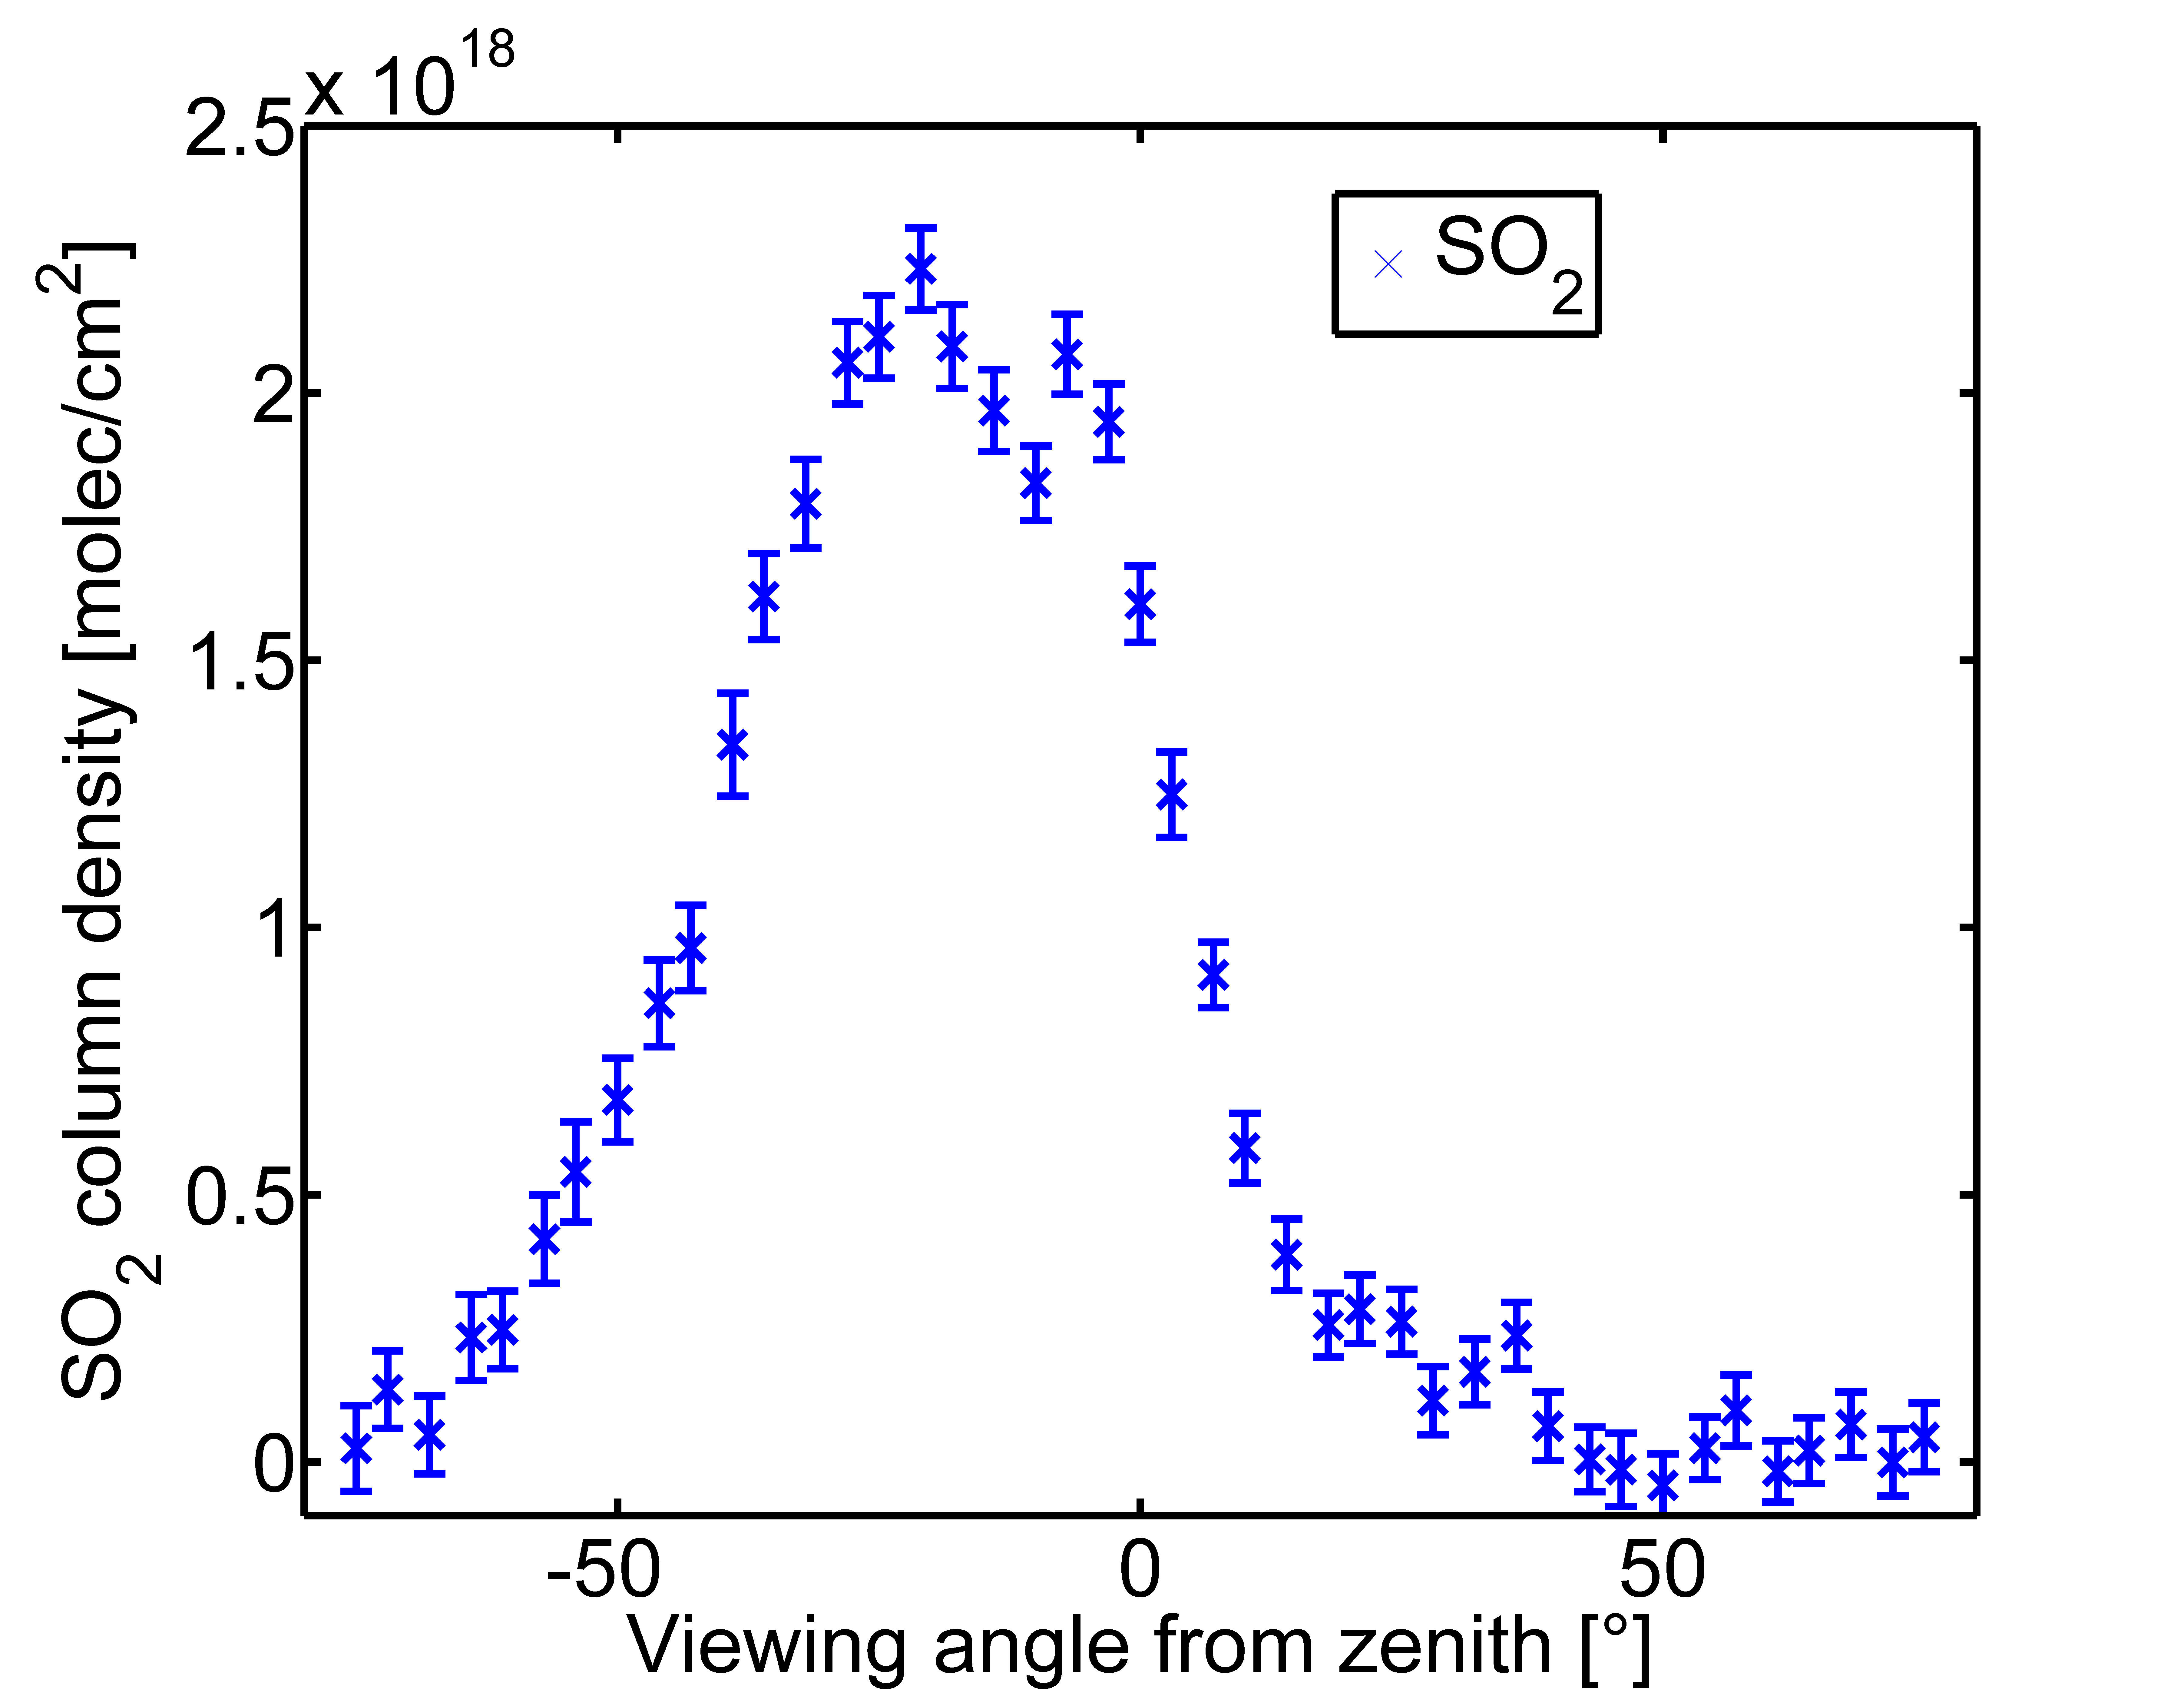
\includegraphics[width=0.49\textwidth]{Bilder/Simon/Bilder_Tung/SO2_Scan_0}}
		\subfigure[]{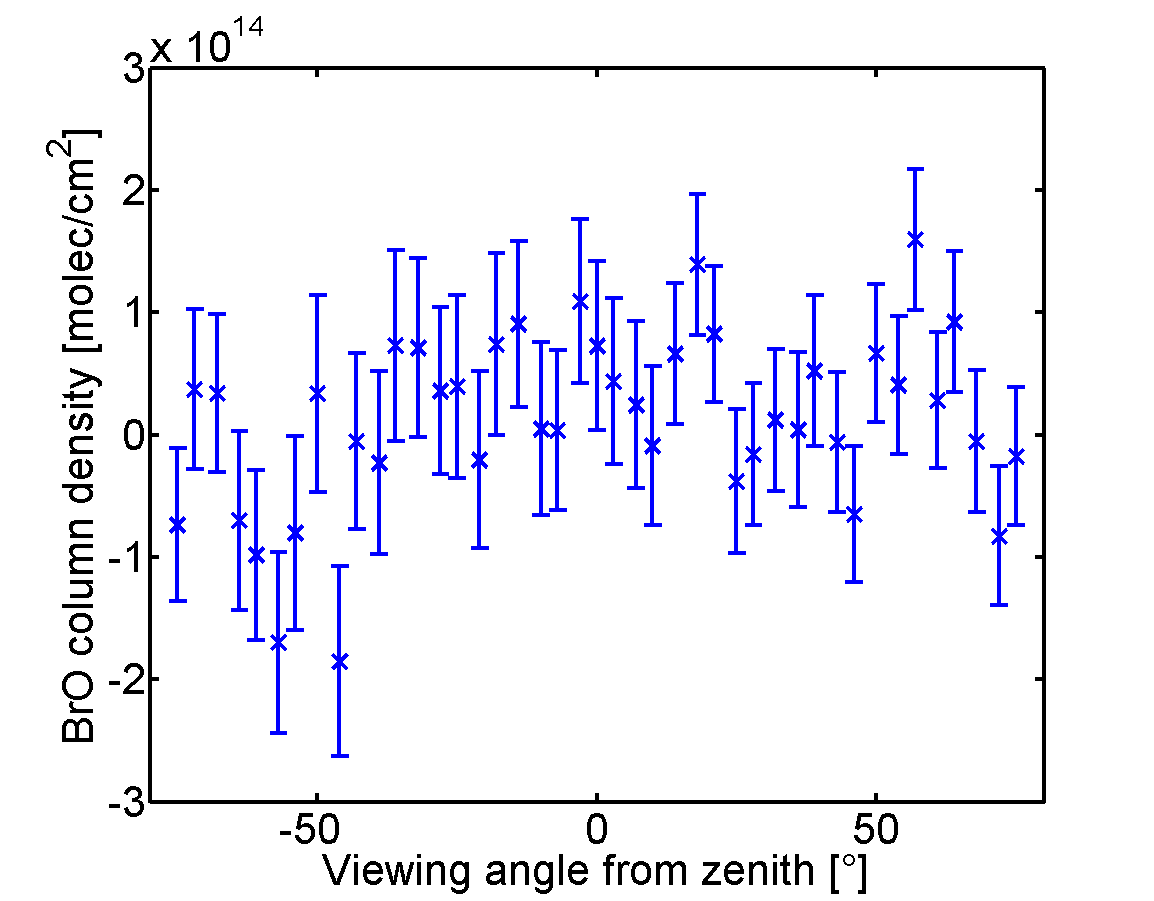
\includegraphics[width=0.49\textwidth]{Bilder/Simon/Bilder_Tung/BrO_Scan}}
		\caption{(a) \ce{SO2} SCD as a function of the elevation angle with error bars resulting from the DOASIS fitting routin. (b) \ce{BrO} SCD as a function of the elevation angle with error bars resulting from the DOASIS fitting routinee  Adapted from \cite{WarnachSimon}}
		\label{fig:plumeref}
	\end{figure}
	%
	In the following we describe the technical implementation of the DOAS approach using the data of NOVAC instruments:\\
	\begin{figure}
		\centering
		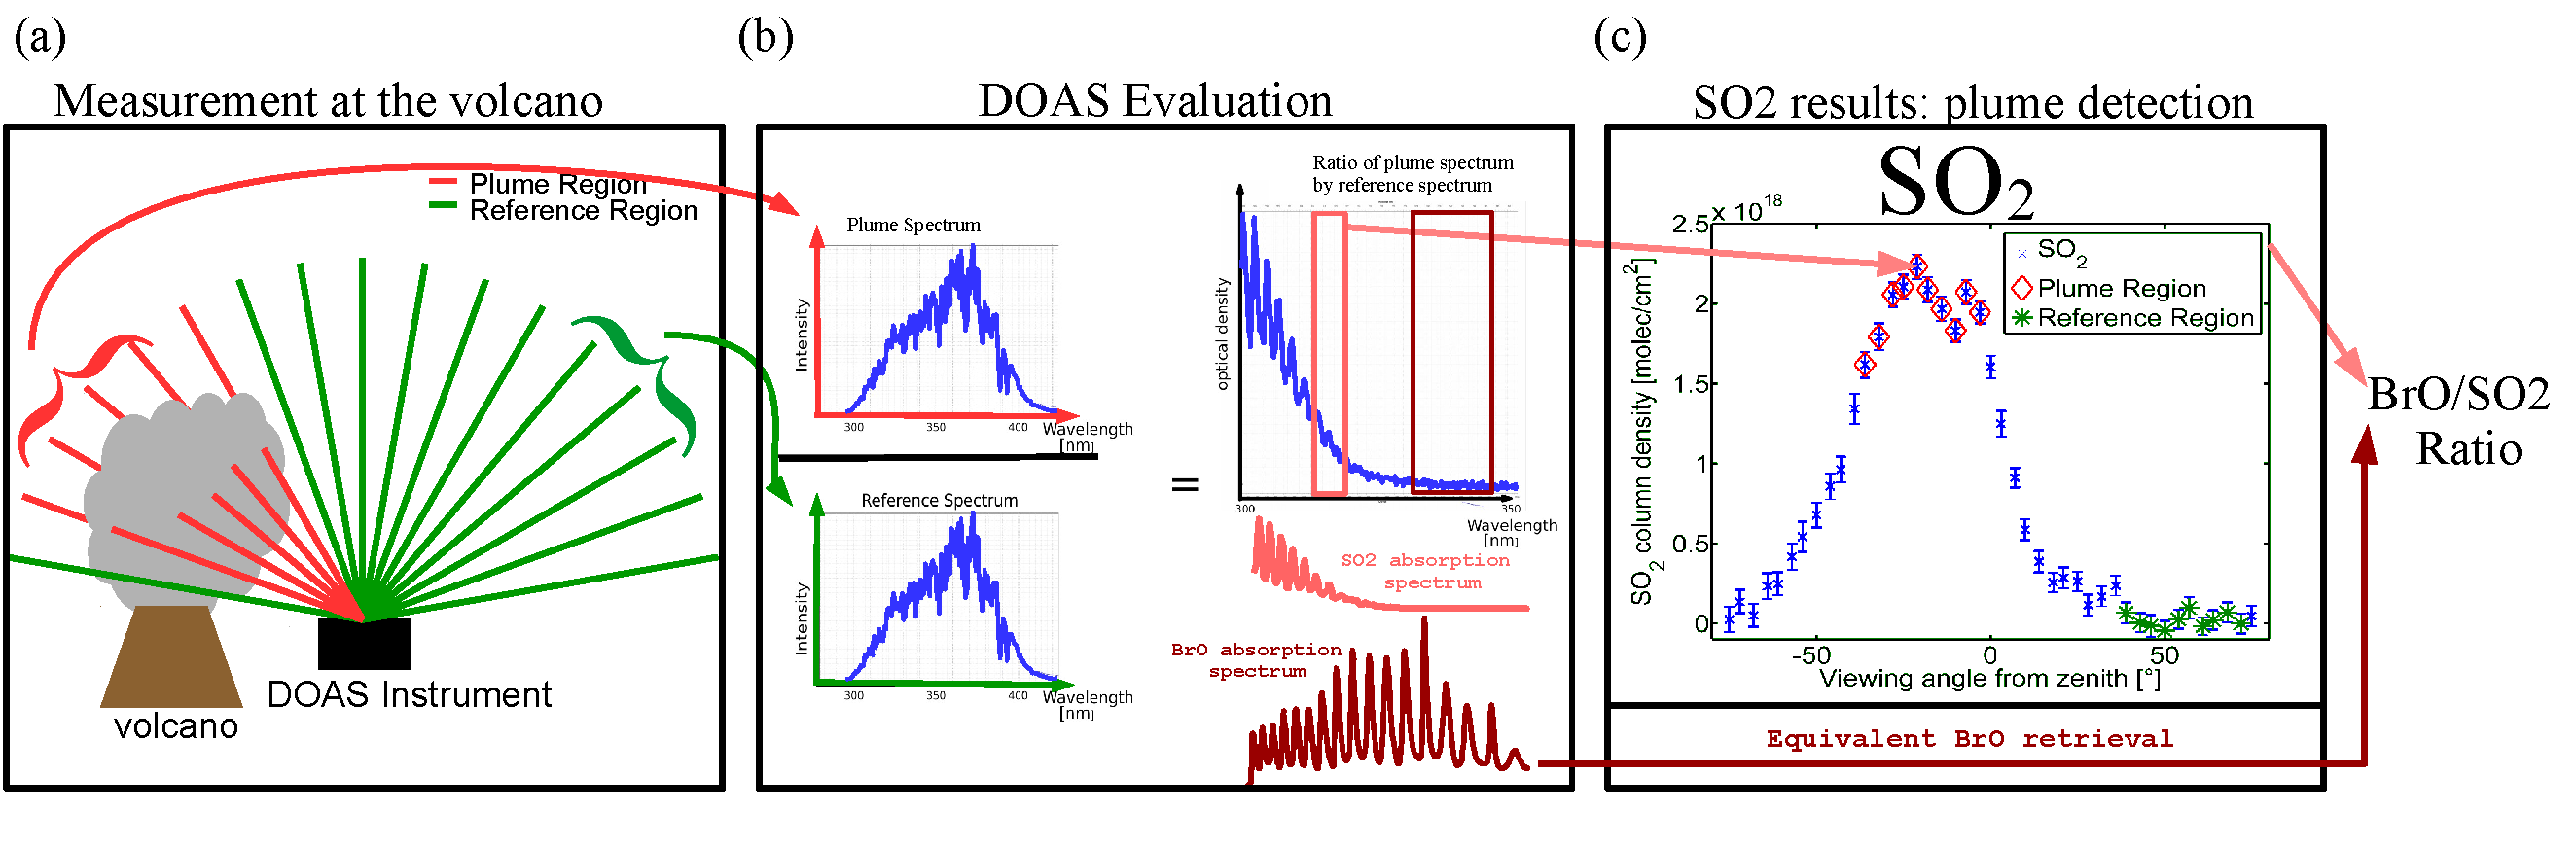
\includegraphics[width=1\linewidth]{Bilder/NOVAC_Eval}
		\caption{NOVAC Evaluation: (a) Measurement at the volcanoe (b) Evaluation of the spectral data with the DOAS routine using the absoption cross sections of BrO and SO2. (c) finding the location of the plume and reference (d) the ratios BrO/SO2 at Tungurahua }
		\label{fig:NOVAC_Eval}
	\end{figure}
	%
	The first step is to correct each spectra of the scan for dark current and offset using the dark current spectrum.
	The next important task is to locate the measurement spectrum in the volcano plume and the reference region. 
	To do so the pre-reference (the spectra recorded at an elevation angle of  0$^{\circ} $) is used to perform the evaluation of the scan spectra recorded at every elevation angle.
	For every spectrum of the scan the so2 differential slant column density (dSCD) with respect to the pre-reference is calculated by the DOASIS fit routine.

	The result is \ce{SO2} dSCD's as a function of the elevation angle. So we can localize the maximum and the minimum of \ce{SO2}
	The location of the \ce{SO2} maximum match with the location of the plume. We assume that the minimum of the \ce{SO2} curve refers to a region outside of the plume which is in most times the case. The \ce{SO2} amount in the earths atmosphere is negligible (see  \cref{chap:so2}) so we take it as a region of zero \ce{SO2}. Now it is possible to locate the plume region as the \ce{SO2} maximum, whereas the minimum of the \ce{SO2} curve the reference region is. \\
	To technically detect the plume region we use a gauss fit of the \ce{SO2} curve.
	To increase the quality and to get a more robust result the sum over several plume spectra is taken. If the gauss curve is too wide we use only the 10 spectra with the highest \ce{SO2} amount. For the reference we use the sum of 10 spectra with the lowest \ce{SO2} amount.\\
	%
%	\begin{figure}
%		\centering
%		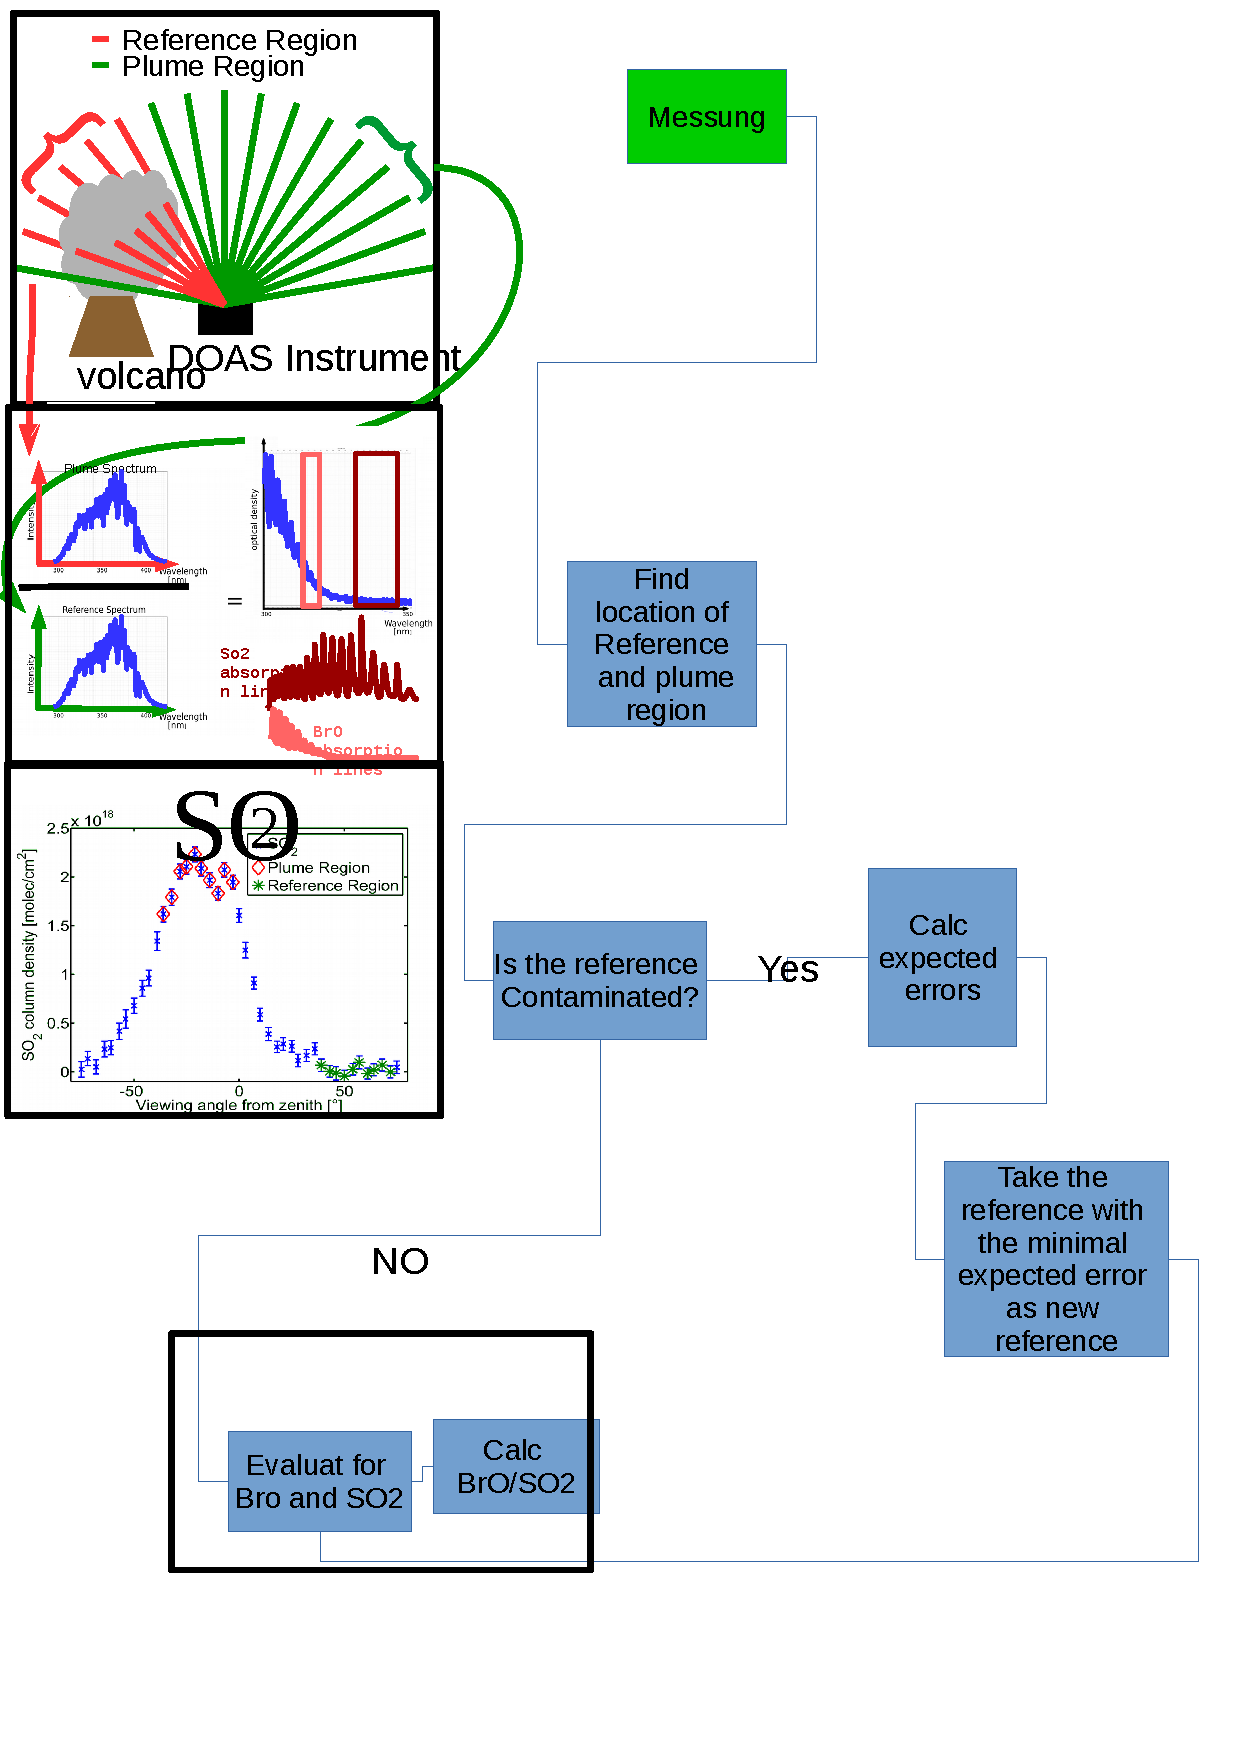
\includegraphics[width=0.7\linewidth]{Bilder/DOAS_Routine}
%		\caption{Sketch of the DOAS Routine }
%		\label{fig:FlussDiag}
%	\end{figure}
	The absolut slant column densities (SCD's) of BrO and So2 can now be calculated with the so found reference and plume spectrum.
	In \cref{fig:plumeref} (a) the SO2 SCD as a function of the elevation angle is shown. The SO2 curve show a clear maximum at the position of the plume at an elevation angle of approximately $-30^{\circ}$ to $0^{\circ}$  and a reference region at an elevation angle of $40^{\circ}$ to $70^{\circ}$. \cref{fig:plumeref} (b): The extrema of the BrO curve are not as distinct as at the SO2 curve. The assumption is, that the BrO of the plume can be found at the same elevation angle as is founded fr the so2. Thus the localization of the plume only need to be done once.
	Since the \ce{BrO} column density is much lower than the \ce{SO2} column density and lies just slightly above the detection limit the plume is hard to detect using the \ce{BrO} column density as it is shown in fig. \ref{fig:plumeref} (b). 
	Therefore we use plume location we found by using \ce{SO2} to evaluate the \ce{BrO} column density.\\
	\Cref{fig:algorithm} (b): shows the routine of adding multiple spectra of consecutive measuring times.\\
	%
	Taking the \ce{BrO}/\ce{SO2} ratio if the column densities are close to zero yields unpredictable and unrealistic results. Thus spectra measured outside of the volcano plume need to be excluded.
	This could be achieved by setting a \ce{BrO} or/and a \ce{SO2} threshold. A reasonable \ce{BrO} threshold need to be at least in the order of the DOAS fit error. But this could lead to elevated \ce{BrO}/\ce{SO2} ratios, since the \ce{BrO} error is often close to the detection limit, and thus exclude all low \ce{BrO} column densities from the evaluation.
	%
	\begin{figure}
		\subfigure[ ]{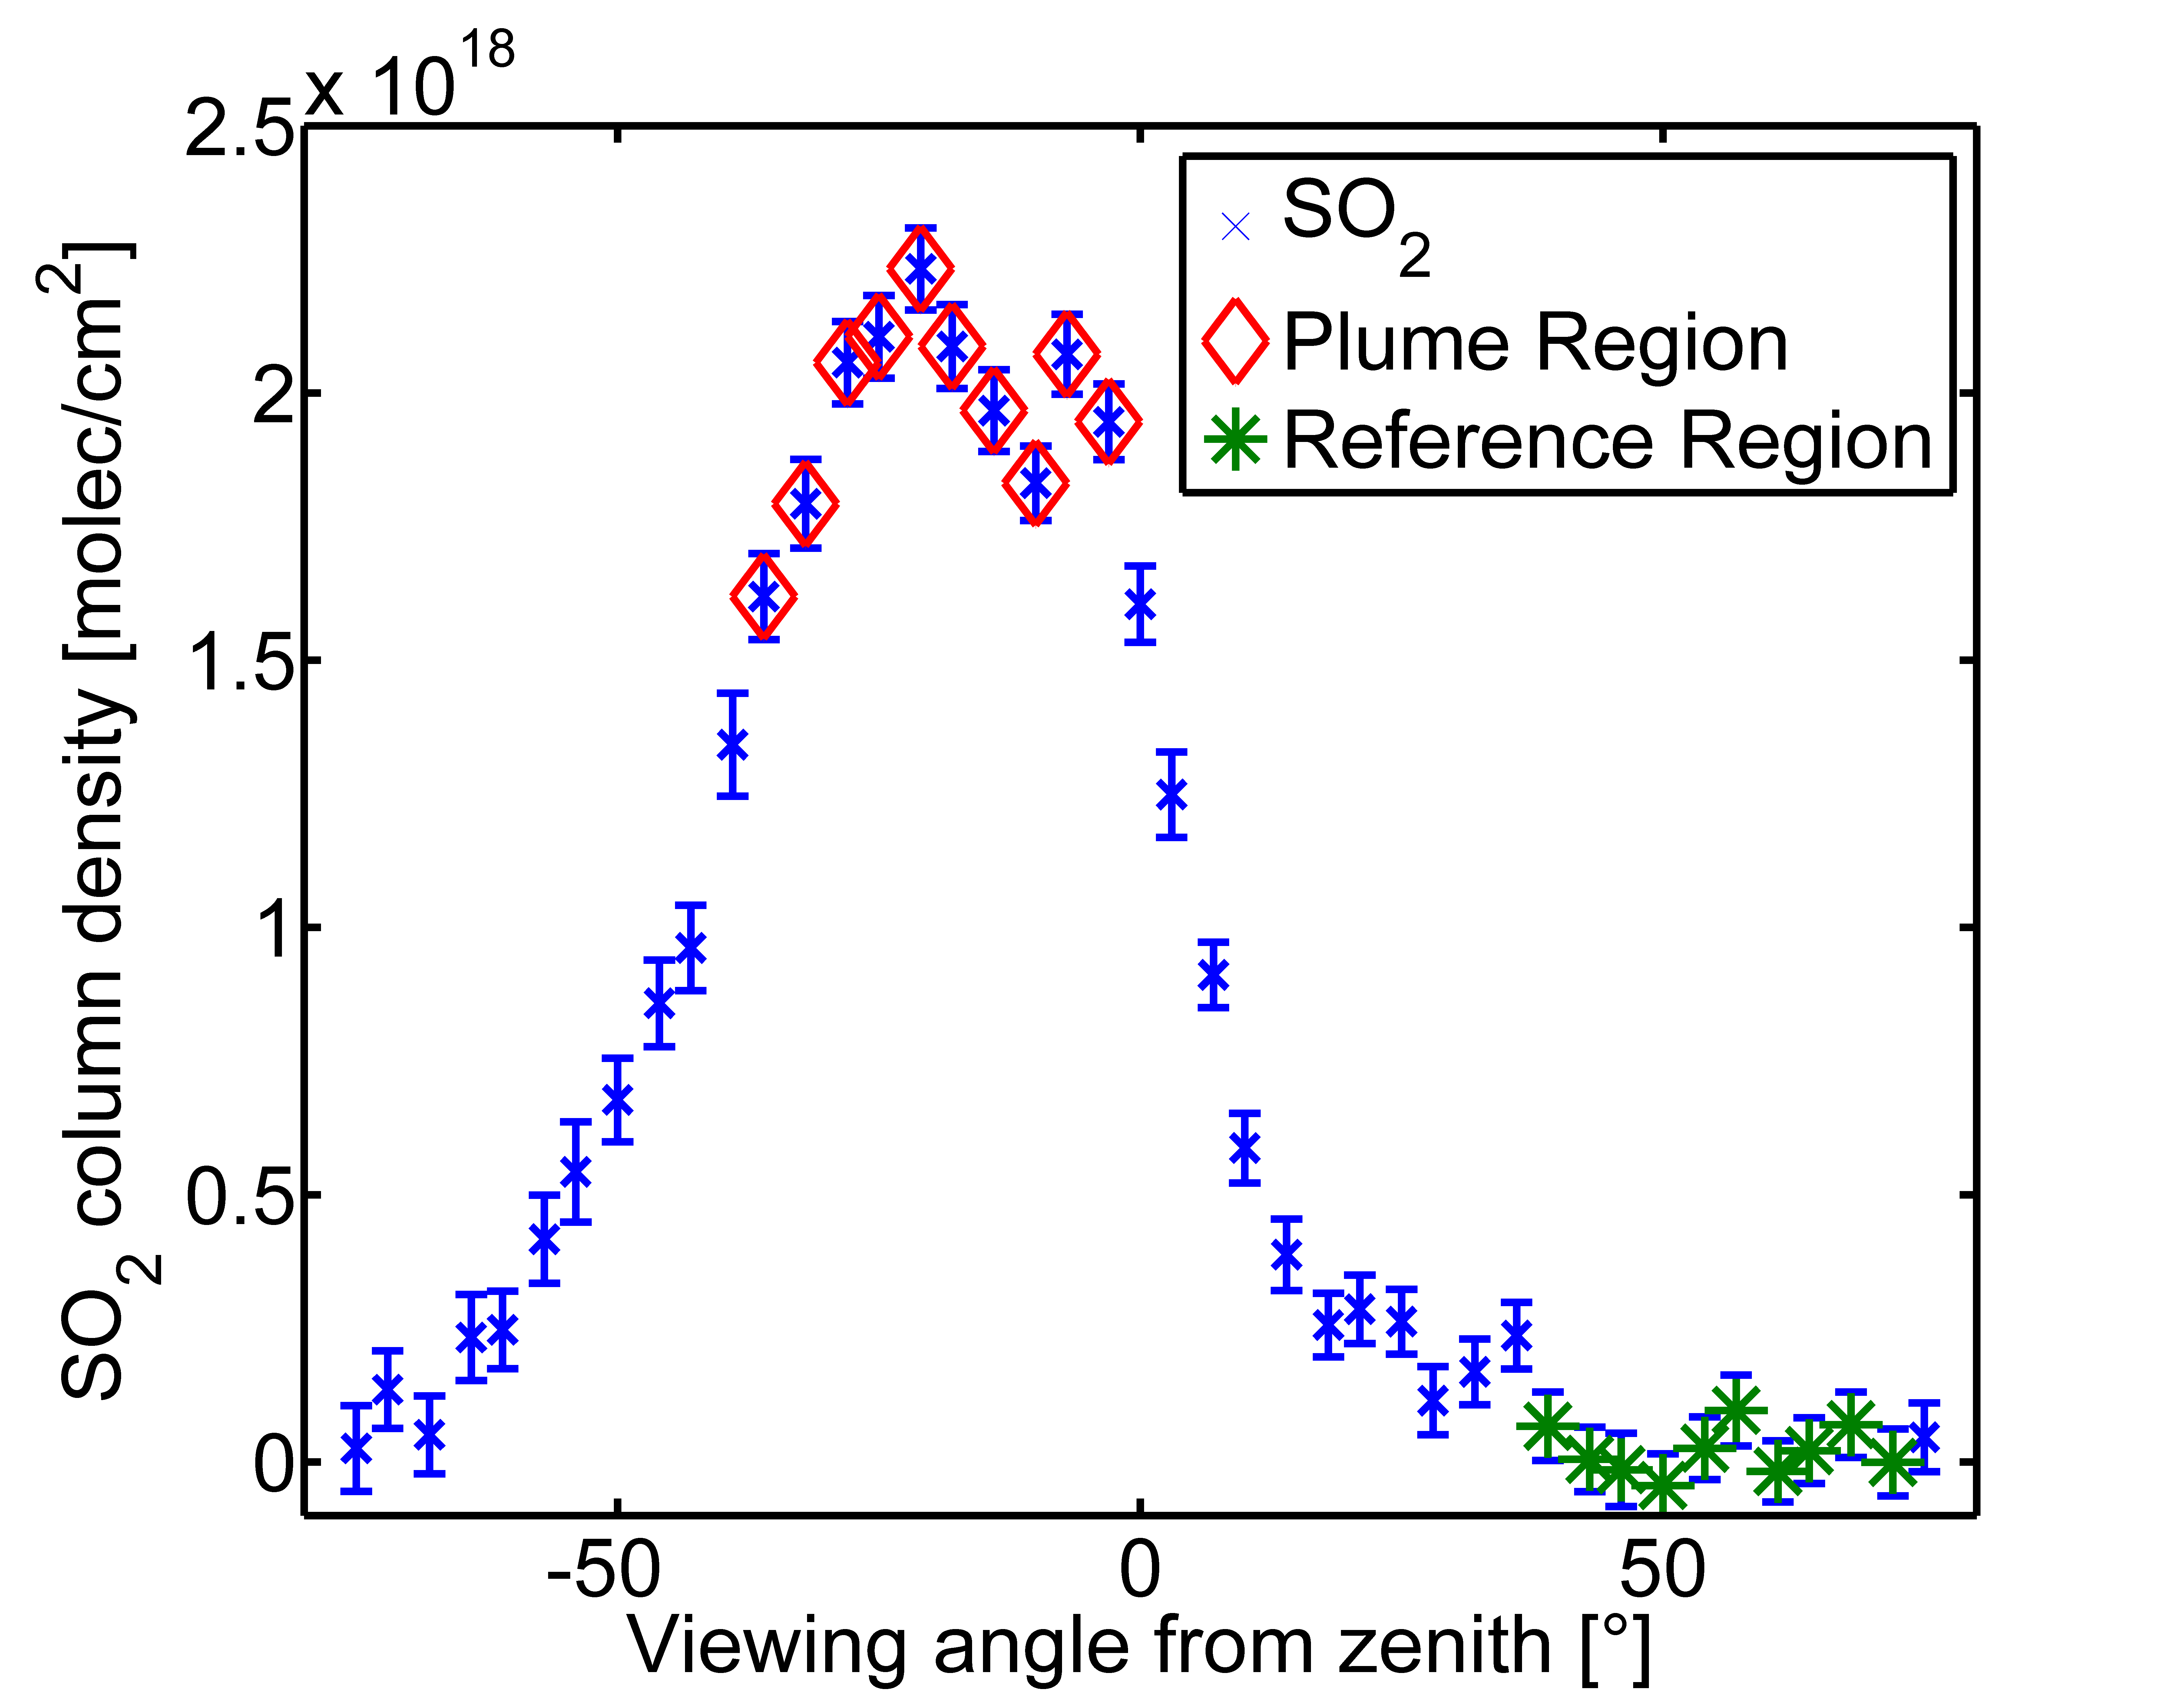
\includegraphics[width=0.5\textwidth]{Bilder/Simon/Bilder_Tung/SO2_Scan}}
		\subfigure[ ]{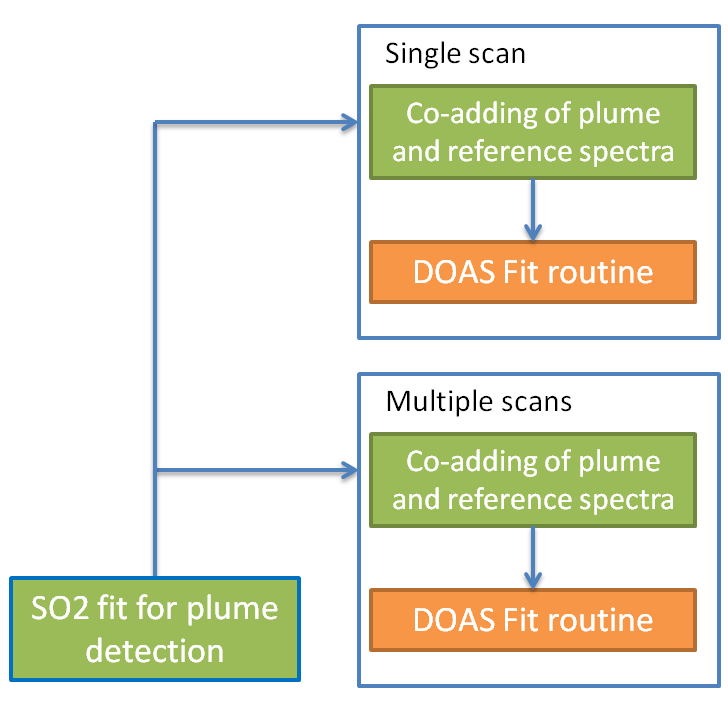
\includegraphics[width=0.47\textwidth]{Bilder/Simon/Bilder_Tung/Algorithm}}
		\caption{(a) \ce{SO2} SCD as a function of the elevation angle. The co-added Plume region is marked with red diamonds, and the co added reference region with green stars. From \cite{WarnachSimon}. (b) Flow chart of the BrO and SO2 evaluation. From \cite{lubcke2014optical}.}
		\label{fig:algorithm}
	\end{figure}
	The other possibility is to set a \ce{SO2} threshold. In this thesis an \ce{SO2} threshold (plume limit) of $7\cdot 10^{17} \frac{molec}{cm^2}$ was used for the selection of spectra for the evaluation of the \ce{BrO}/\ce{SO2} ratio. $7\cdot 10^{17} \frac{molec}{cm^2}$ is a relatively high column density. However this this approach assures that no significant amount of gases will be filtered out, therefore the BrO/So2 will not be significantly influenced \citealp{lubcke2014bro} and that all accepted measurement spectra will be inside of the volcano plume. 
	
	\section{Contamination Problem\label{Chap:Cont}}	
	It might occur that in rare (ca. 10\% of the data) scenarios, the
	volcanic plume covers the whole scan region.
	This could happen if for example the volcanic plume of the day before still extend over the hole scan area as a consequence of windless conditions.
	In consequence, the reference	is contaminated with volcanic trace gases. Thus the gas amount is underestimated by the NOVAC-Evaluation: In \cref{fig:contaminated} we see an example from April 2011 (Tungurahua) where the reference region is contaminated by volcanic trace gases. The blue \ce{SO2} curve shows our calculations with the NOVAC-Evaluation, but since there is still \ce{SO2} in the reference region, the assumption, that the \ce{SO2} amount could be set to zero in the reference region is wrong. The red curve shows the real \ce{SO2} curve, which lies significantly above the NOVAC -curve. Contamination occur in approximately 10$\%$ of the data.\\
	\\
		\begin{figure}
			\centering
			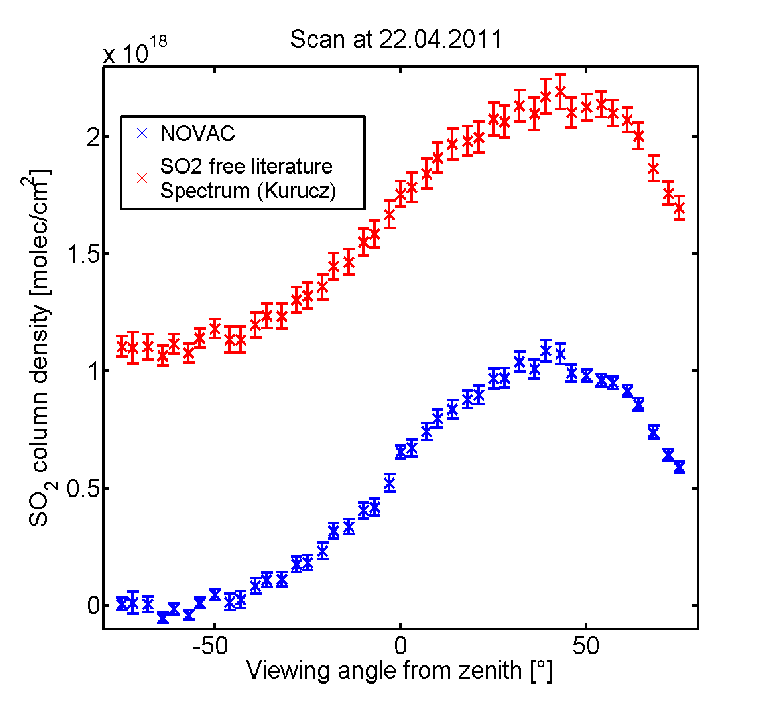
\includegraphics[width=0.7\linewidth]{Bilder/contaminated}
			\caption{Scan with a contaminated reference spectrum from April 2011. From \cite{WarnachSimon}}
			\label{fig:contaminated}
		\end{figure}
	If the reference region is for any reason
	contaminated by volcanic trace gases, the reference spectrum has to be
	replaced by a volcanic-gas-free reference. Alternative spectra are a
	theoretical solar atlas spectrum or a volcanic-gas-free reference
	spectrum recorded by the same instrument.\\ 
	%
	\\
	%
	In the following we will discuss both of these options:
	%
	\subsection*{Evaluation using a Solar Atlas Spectrum \label{kuruz}}
	An alternative to choose the region with the lowest column density as reference region is to use a theoretical high resolution solar atlas spectrum as reference \cite{chance2010improved}.
	The use of a theoretical solar atlas spectrum as a reference which is completely volcanic-trace-gases-free was first proposed by \cite{lubcke2014bro}.
	The advantage of using a solar atlas spectrum as reference is, that we know that there are no volcanic trace gases, we do not need to assume, that the minimum \ce{SO2} amount is zero. The disadvantage is, that using a solar atlas spectrum comes along with a drawback of precision: A theoretical solar atlas spectrum is far more precise than the spectra of the NOVAC instruments therefore the instrument functions need to be modeled and added to the retrieval.\\ 
	The reduction of precision is acceptable for the
	\ce{SO2} retrieval but not suitable for a \ce{BrO} retrieval because then most data would be below the detection limit.\\
%
\\
%
	Possible contaminations can be checked
	by a theoretical solar atlas spectrum to evaluate the \ce{SO2} amount in the reference.
	%
	\subsection*{Evaluation using a Spectrum of the same Instrument}
	An alternative reference spectrum could be a volcanic-gas-free reference
	spectrum recorded by the same instrument. When using such a reference several problems occur:\\
	As described in \cref{NOVAC} the instruments used in NOVAC do not include features like temperature stabilisation due to that the measurements are not independent from external parameters. 
	So we need to choose a reference recorded at similar conditions with respect to meteorology and	radiation as well as in the temporal proximity due to instrumental changes with time and ambient conditions. Ideally the external conditions should be equal to the conditions when the plume was recorded.\\
	\\
	%
	\\
	In this work we will combine both options in order to
	achieve both, enhanced accuracy but still maximum possible precision of
	the \ce{SO2} and \ce{BrO} retrievals. So we use the solar atlas spectrum to check for 
	contamination and a reference spectrum recorded in temporal proximity by the same instrument as reference.\\
	\\
	Thus if contamination occurs it is possible to choose from a list of gas free alternative references. In theory, for ideal instruments al references should lead to the same results for the gas retrievals. But instruments are imperfect (see \cref{NOVAC}) thus the reference need to be chosen carefully an order to improve the results.\\
	%
	\\
	In the following we will discuss how to find the an optimal reference from another scan automatically.
	
	\begin{figure}
		\centering
	%	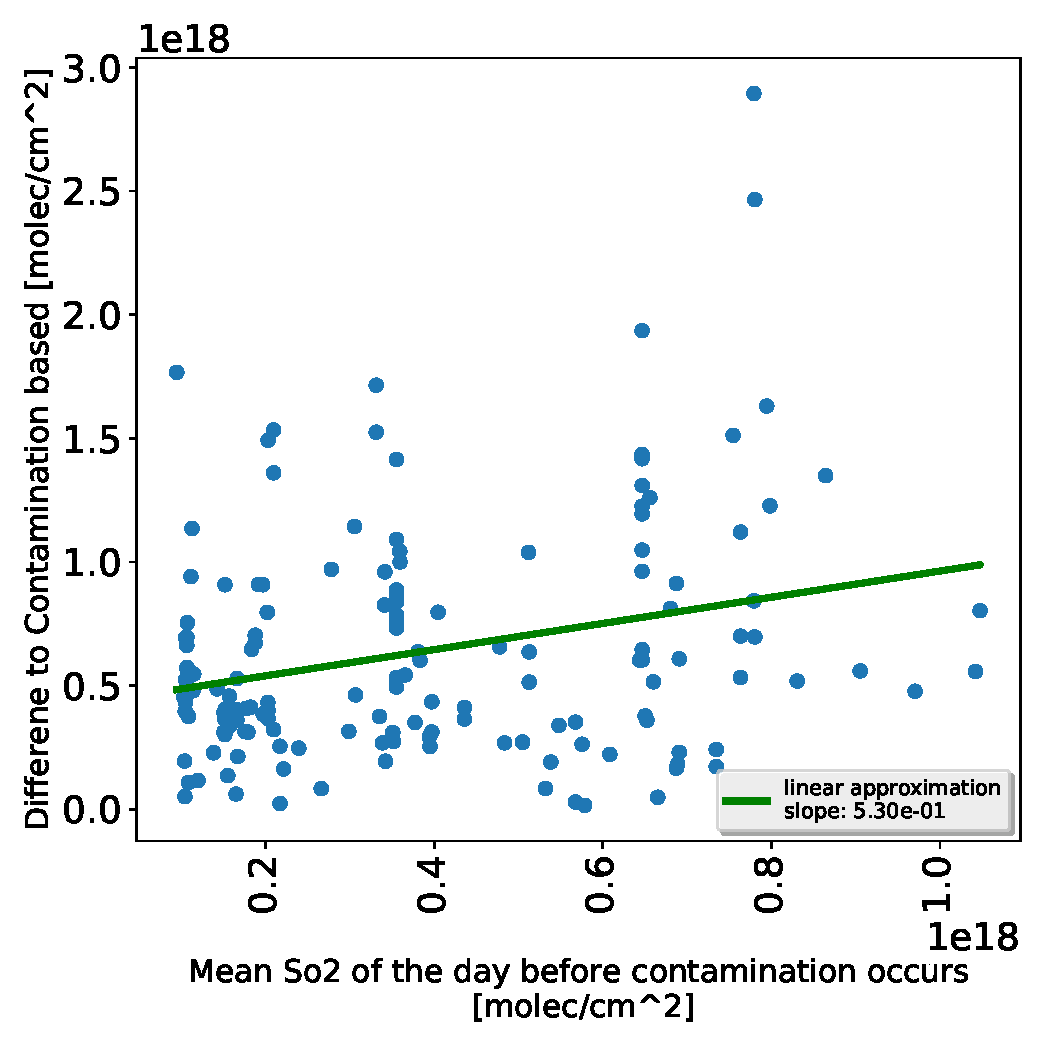
\includegraphics[width=0.7\linewidth]{E:/Masterarbeit/Analyse_Contamination/contaminationdependency_so2}
		\caption{}
		\label{fig:contaminationdependencyso2}
	\end{figure}
	\begin{figure}
		\centering
%		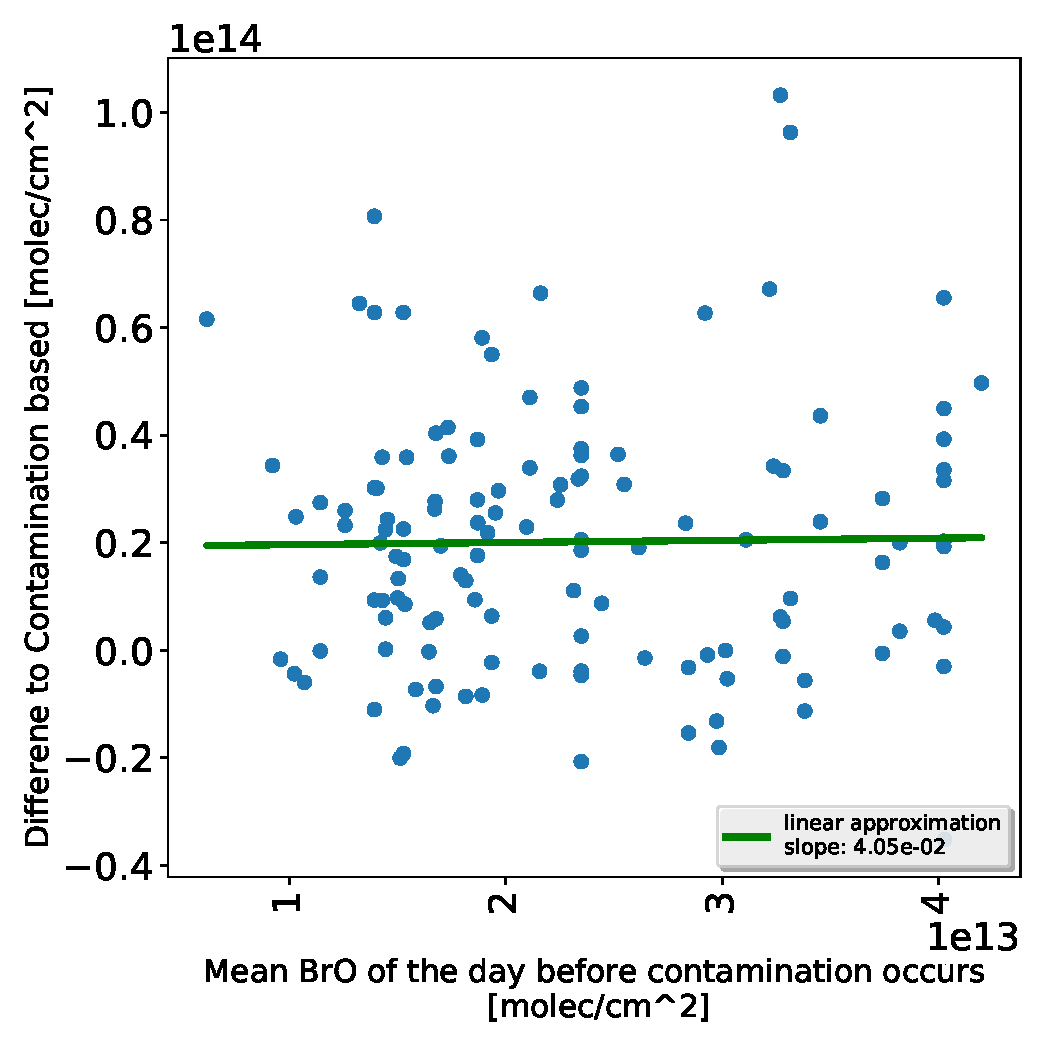
\includegraphics[width=0.7\linewidth]{E:/Masterarbeit/Analyse_Contamination/contaminationdependency_bro}
		\caption{}
		\label{fig:contaminationdependencybro}
	\end{figure}
	\begin{figure}
		\centering
%		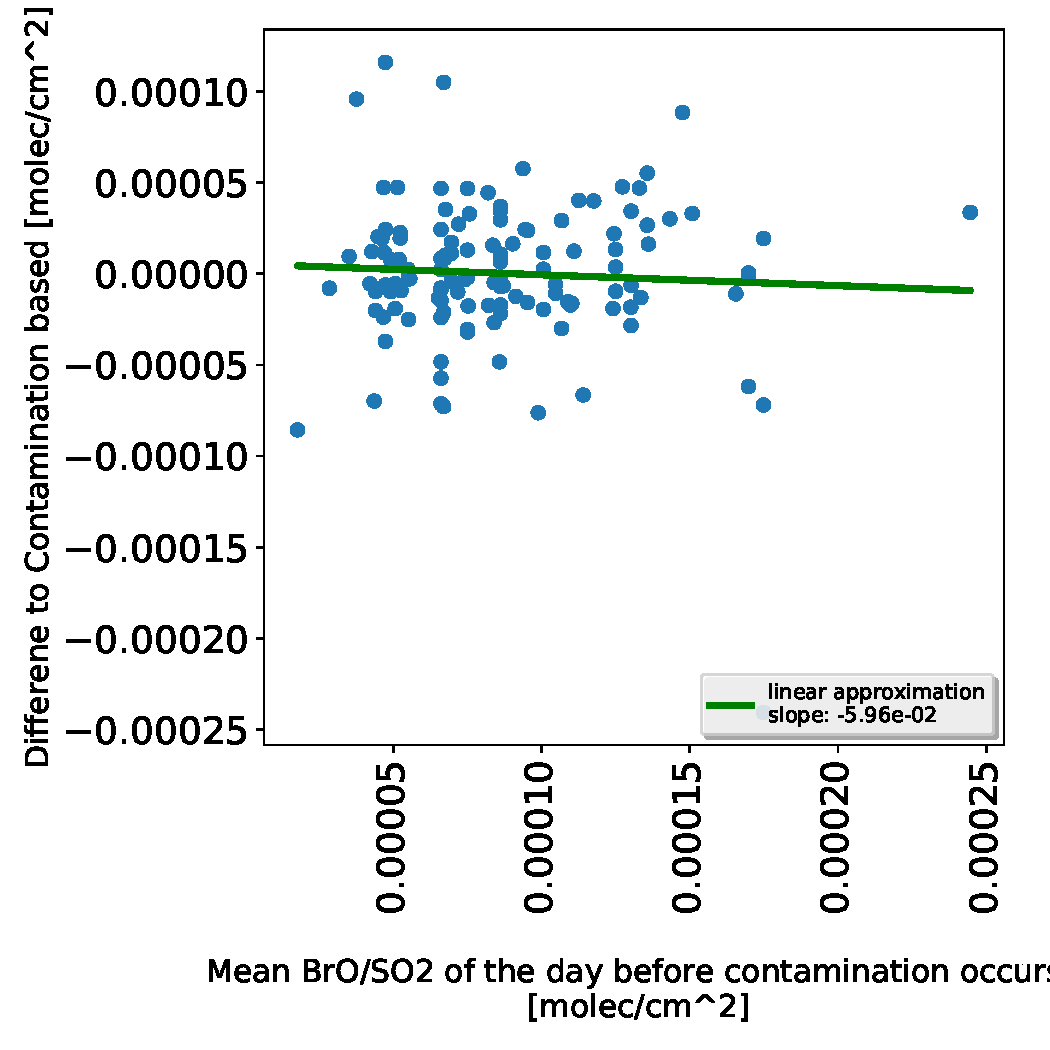
\includegraphics[width=0.7\linewidth]{E:/Masterarbeit/Analyse_Contamination/contaminationdependency_ratio}
		\caption{}
		\label{fig:contaminationdependencyratio}
	\end{figure}
	\chapter{BrO Evaluation and its limitations}
	This chapter discuss the evaluation of BrO by DOAS Instruments of NOVAC.\\
	Compared to the SO2 SCD (magnitude of \ce{SO2} at Tungurahua $\approx 1e^{18}$, \cite{WarnachSimon}) the BrO SCD is rather low. This results in a larger uncertaintiy of the BrO SCD. Most of te BrO data are below the detection lime of BrO$_{err}$/BrO$_{value}$<1/4. SCD's of So2 are in almost all cases (?????\% of the data) above the detection limit. 
	Choosing a different reference than the reference meausred at the same tima as the plume results in 99\% of all data in an increasing absolut error. 
	%
	Thus an \ce{BrO} Error which is smaller than the "Same Time Error" will not be possible to retrieve when calculating the gas slant column densities with a different reference. However the aim is to get the smallest possible error to achieve a maximal amount of reliable BrO/SO2 ratio data.\\
	\\
	References where the surrounding conditions e.g temperature or cloudiness are equivalent with the surrounding conditions of the  plume measuring lead to a small error.
	Since we want to get the \ce{BrO}/\ce{SO2} we need to maximize the accuracy of BrO.
	Therefore the aim is to choose the reference with respect to the \ce{BrO} error, to minimize the \ce{BrO} In the following, we will take a closer look at the dependence of the \ce{BrO} error on external parameters. 
	%
	\section{\ce{BrO} Error dependence on external parameters \label{Chap:BROErr}}
	%HOW IS THE ERROR CALCULATED AND WHY AND DETECTION LIMIT (PLATT \& STUTZ)
	The measurement and evaluation depends on the surrounding conditions like temperature or cloudiness \cite{lubcke2014optical}\\
	As a result the surrounding conditions need to be taken into account if choosing a new reference.\\
	The better the surrounding conditions of the time where the reference is measured coincide with the conditions of the time when the plume is measured, the lower is the \ce{BrO} error \\
	\\

	The surrounding conditions that are considered in this thesis are: 
	\begin{itemize}
		\item Temporal Difference
		\item Temperature, 
		\item Colorindex, 
		\item Exposure Time, 
		\item Elevation Angle, 
		\item Daytime 	
	\end{itemize}
	The analysis of these external parameter will be done for spectra recorded at Tungurahua and Nevado Del Ruiz. At Tungurahua three instruments with data recorded in the time span from July in 2008 to August in 2009 are used. Nevado Del Ruiz contributes with two instruments in the time from the end of 2009 to the end of 2011.
	
	In this time span at Tungurahua 1647 "multi-add" spectra from the pillate instruments where recorded, so we get approximately 1646$^2$ plume reference pairs, the corresponding differences in the external parameter and their associated \ce{BrO} error.
	
	
	\subsection{Temporal Difference}
	\begin{figure}
		\centering
		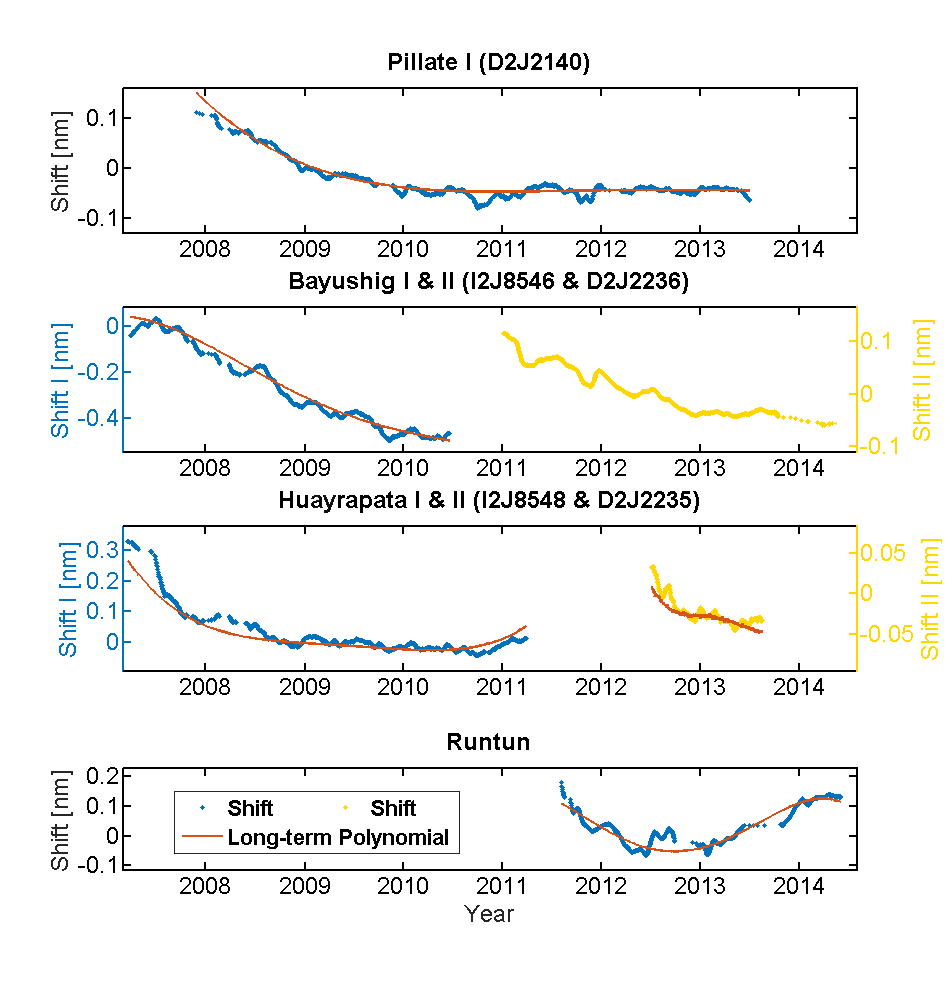
\includegraphics[width=1\linewidth]{Bilder/Simon/Bilder_Tung/Drift_Komplett_NEW}
		\caption{Wavelength shift over the time. The shift is shown for six NOVAC- instruments from Tungurahua. The red and yellow dots show the running mean about 20 days. Red line indicates a temperature independent long term polynomial. From \cite{WarnachSimon}}
		\label{fig:driftkomplettnew}
	\end{figure}
	%
	\begin{figure}
		\subfigure[]{
			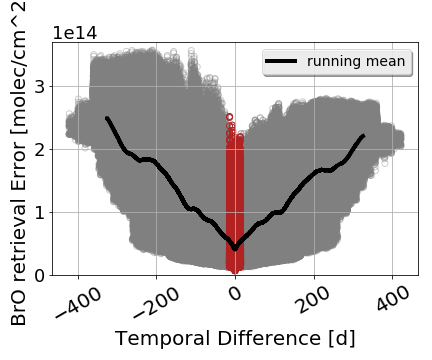
\includegraphics[width=0.5\linewidth]{Bilder/Datum}}
		\subfigure[]{
			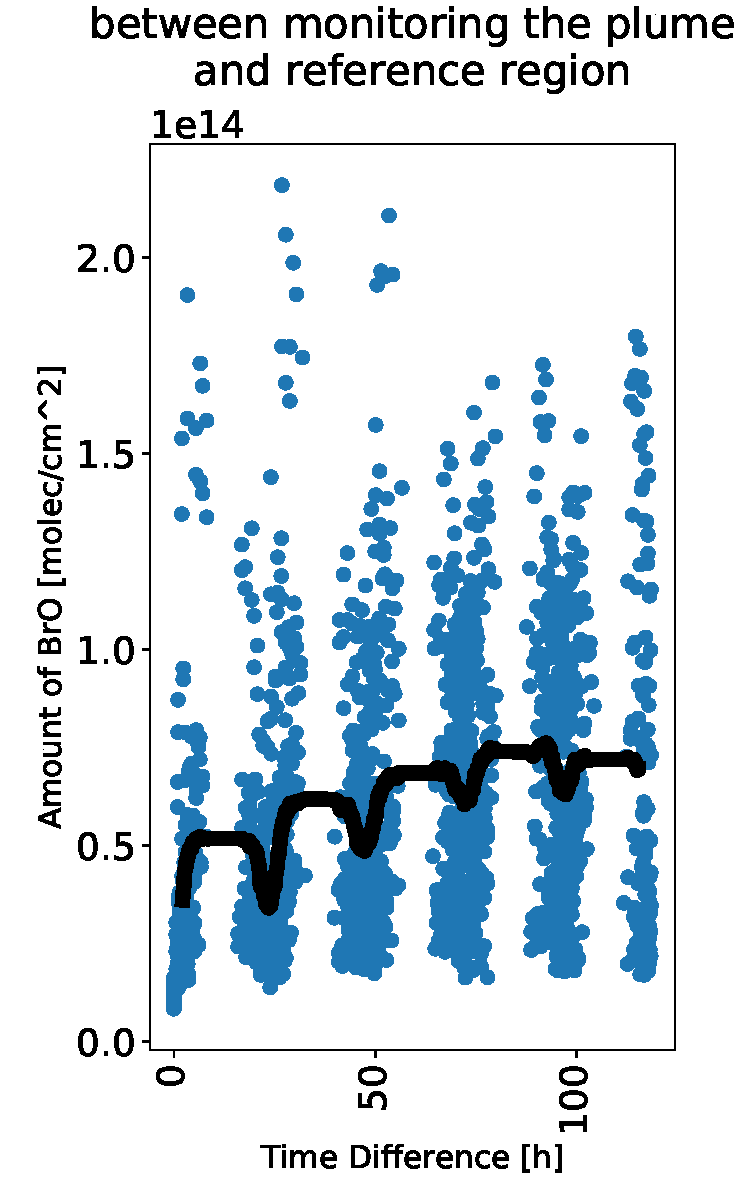
\includegraphics[width=0.5\linewidth]{Bilder/Datum_100h}}
		
		\caption{The BrO error as a function of the temporal difference shown for the Pillate instrument from Tungurahua (2008-2009). (a) Temporal differences up to 400 days are shown. (b) Temporal differences below 120h; periodical BrO error evolution indicates the impact of the daytime}
		\label{fig:dat}
	\end{figure}
	Due to instrument drifts the fit quality decreases with the time difference between recording the plume and the reference. This could be a result of a wavelength shift over time which was observed by \cite{WarnachSimon}.\cite{WarnachSimon} suggested the drift is caused by a hysteresis effect. \Cref{fig:driftkomplettnew} show the wavelength shift as a function of the time for six NOVAC instruments located at Tungurahua in the time between 2008 to 2014. For the analysis in thesis data of Tungurahua between 2008 to the mid of 2009 are used. \Cref{fig:driftkomplettnew} shows a rather steep drift in this time interval. \cite{WarnachSimon} observed a decrease of the shift after initial negative drift after the first 2 years at Pillate. Thus it could be that the temporal difference could become less important for old instruments. For the following discussions we used data of Pillate from 2008 to 2009.\\
	%
	When using reference and plume spectra of the same time, these effects are cut out since the shift is equal for the plume and reference spectrum, For increasing temporal different between reference and plume measurement time the fit quality decreases and thus the BrO Error\\
	In \cref{fig:dat} the \ce{BrO} Error as a function of the time difference between recording the plume and the reference is shown. The running mean is drawn with a black line. \\
	In \cref{fig:dat} (a) it can be seen that a large temporal differences result in an increase of BrO Error of more than 600\%. BrO Errors of such magnitudes are too large for our purposes therefore it is usefull to define a maximal temporal difference. Furthermore it can be seen that the evolution of the BrO error with the temporal difference is symmetric around zero, thus it is not necessary to distinguish between positive or negative temporal differences.\\
	%
	
	 \cref{fig:dat} (b) shows the evolution of the BrO Error for a maximal temporal difference of 120 hours. It is only possible to record data during daytime. This couses the lack of data at some temporal differences. A periodic decrease of the BrO error can be seen. This is a result of a decrease of the BrO error when the surrounding conditions coincidence. In this case the daytime coincidence couses the BrO error decrease, for further discussion of the daytime see \cref{chap:daytime}.\\
	 \cref{fig:dat} is created by using the data only from the Pillate instrument at Tungurahua.\\	
	%
	\textcolor{blue}{To evaluate the maximal time difference, were we still get reliable results we calculated for all possible reference-plume pairs the corresponding \ce{BrO} Error. With this data we are able to find for all plume spectra the associated reference where the \ce{BrO} Error is minimal. In \cref{Histogram} a histogram is plotted with the probability of picking the best reference as a function of the time difference. Obviously the best results are if the day of measuring the reference is the same day as measuring the reference that means, if the time difference is smaller than one day. We allow all time difference which are in one sigma area. }\\
	%
	We found out that the time interval where it is still reasonable to use references is about 14 days. Therefore we only use references where the recording time difference between plume and reference is smaller than two weeks. When using a references with a temporal difference to the plume of more than 14 days the probability, that the fit quality and thus the \ce{BrO} error increases to much for our purposes. \\
	For the following analysis of external parameters all temporal differences are below 14 days.
	%
	\begin{figure}		
		\subfigure[]{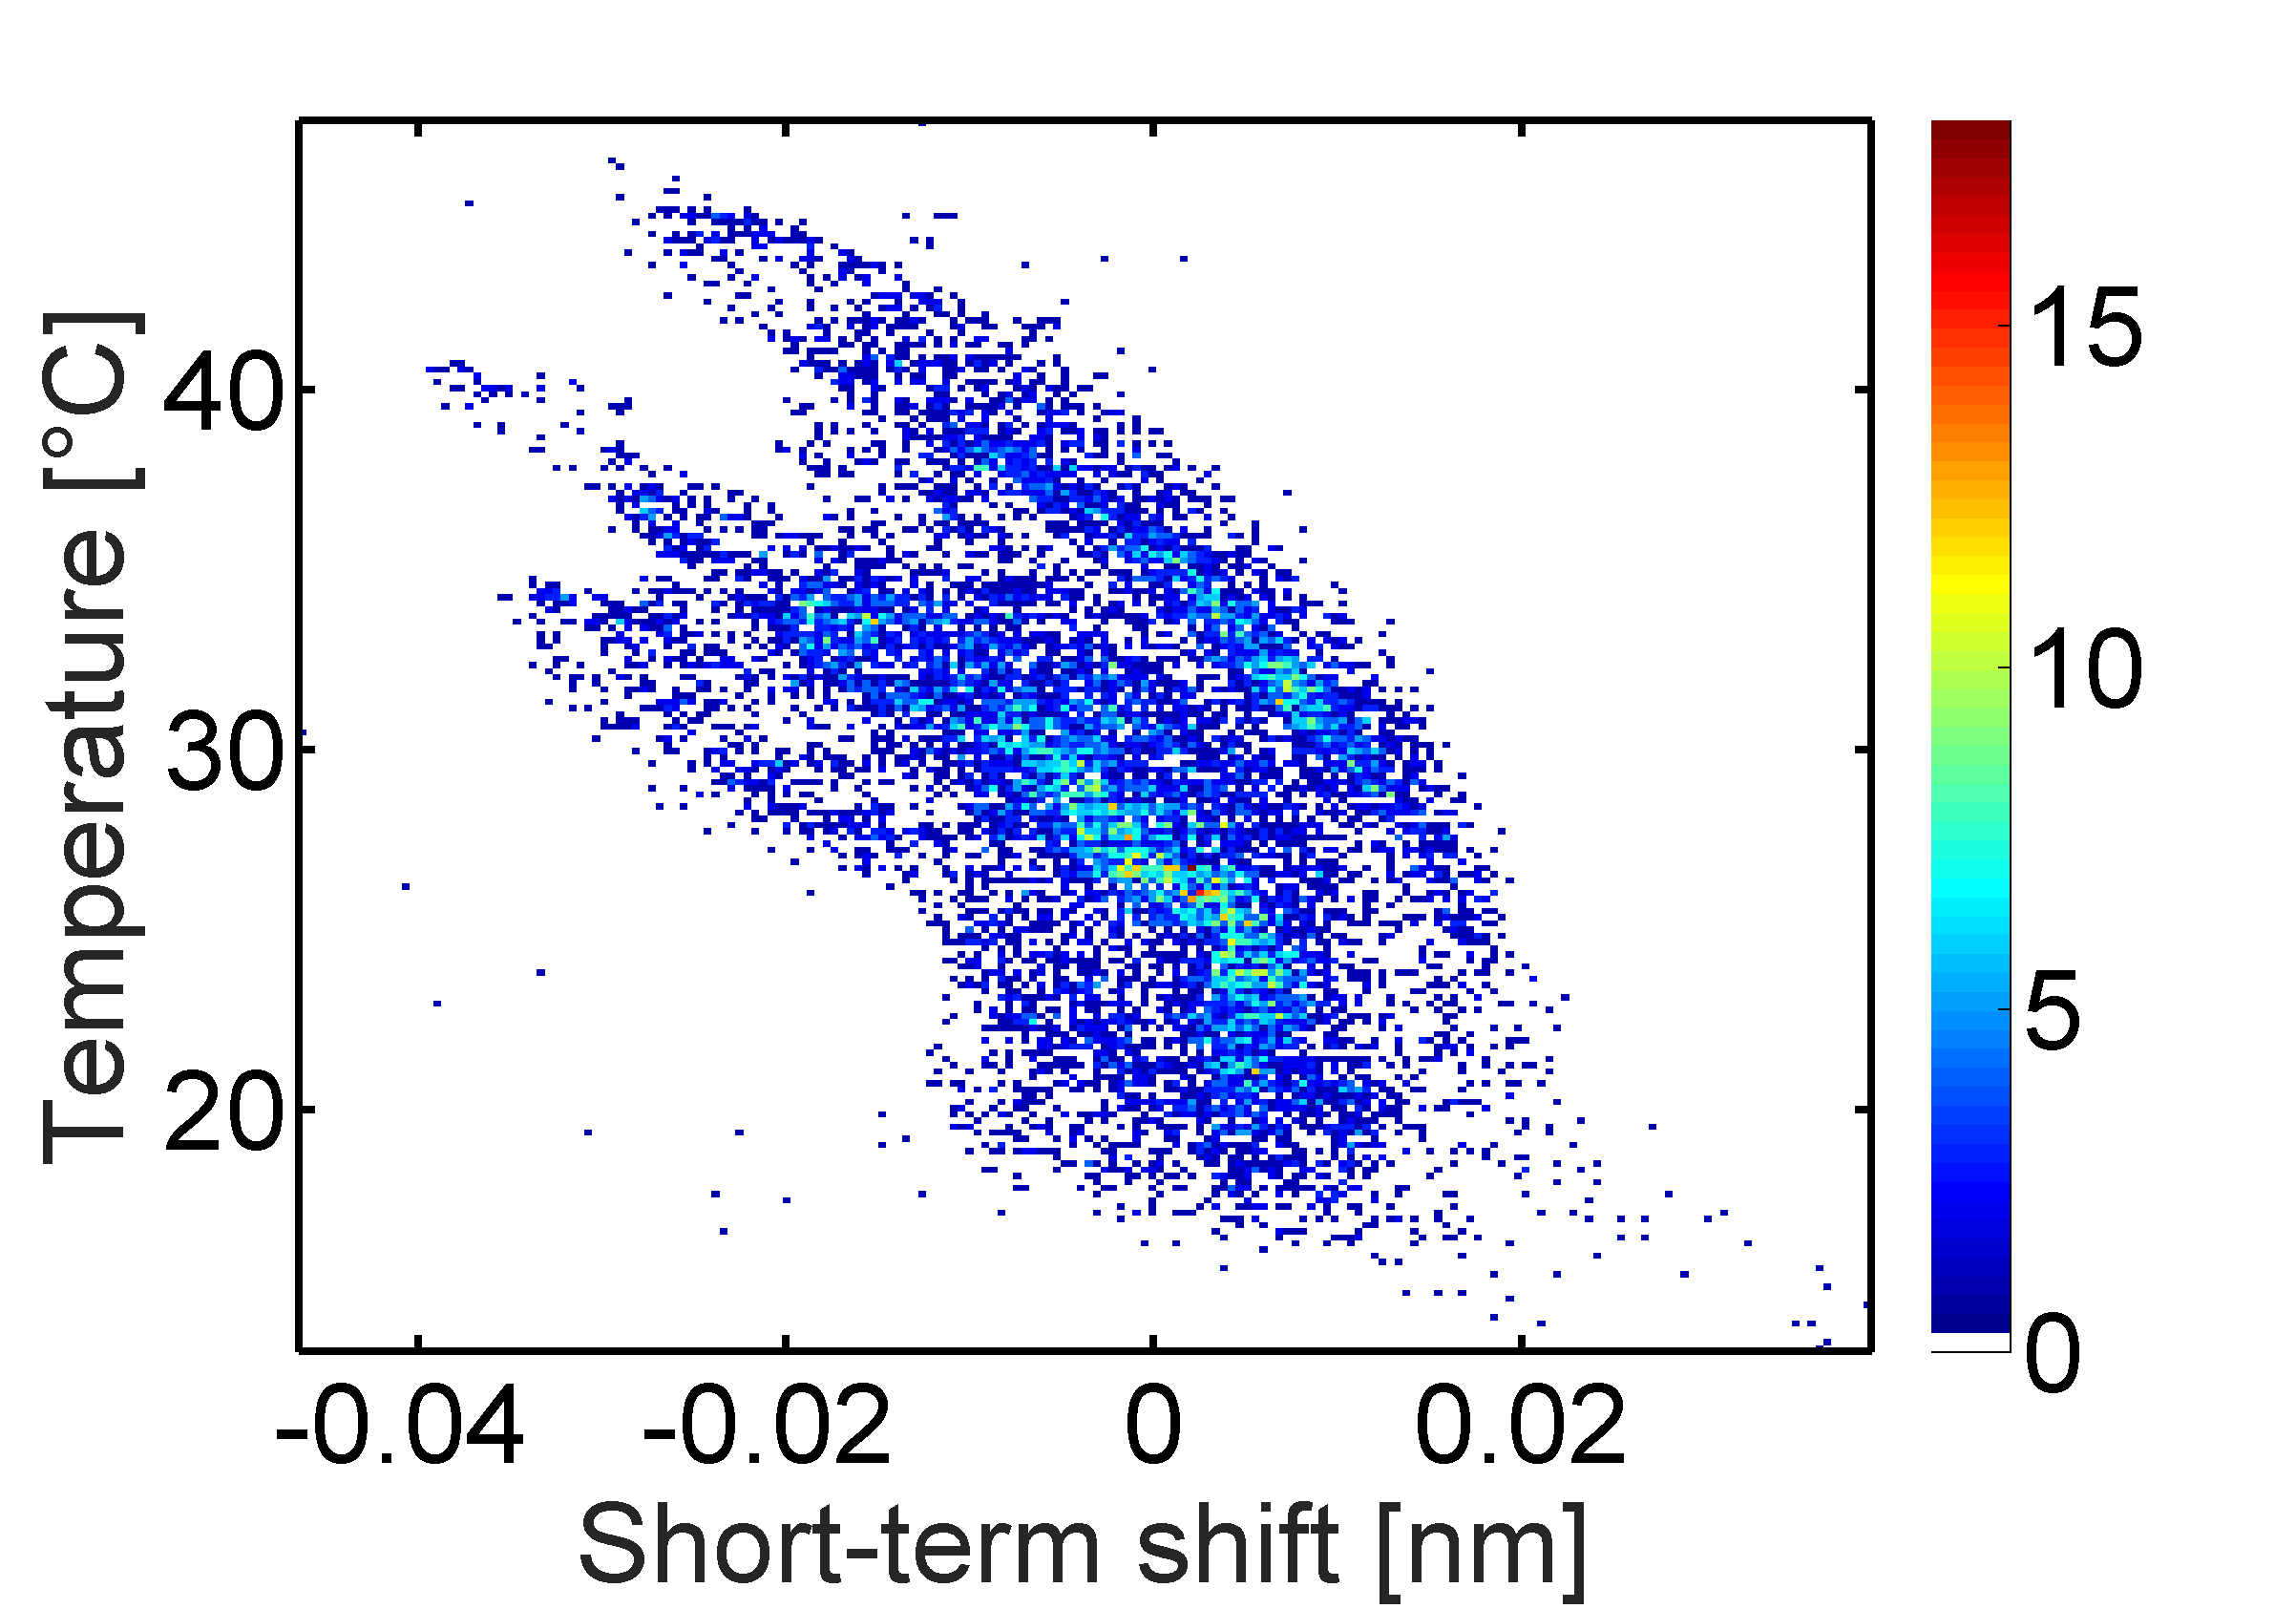
\includegraphics[width=0.49\textwidth]{Bilder/Simon/Bilder_Tung/D2J2140_Before}}
		\subfigure[]{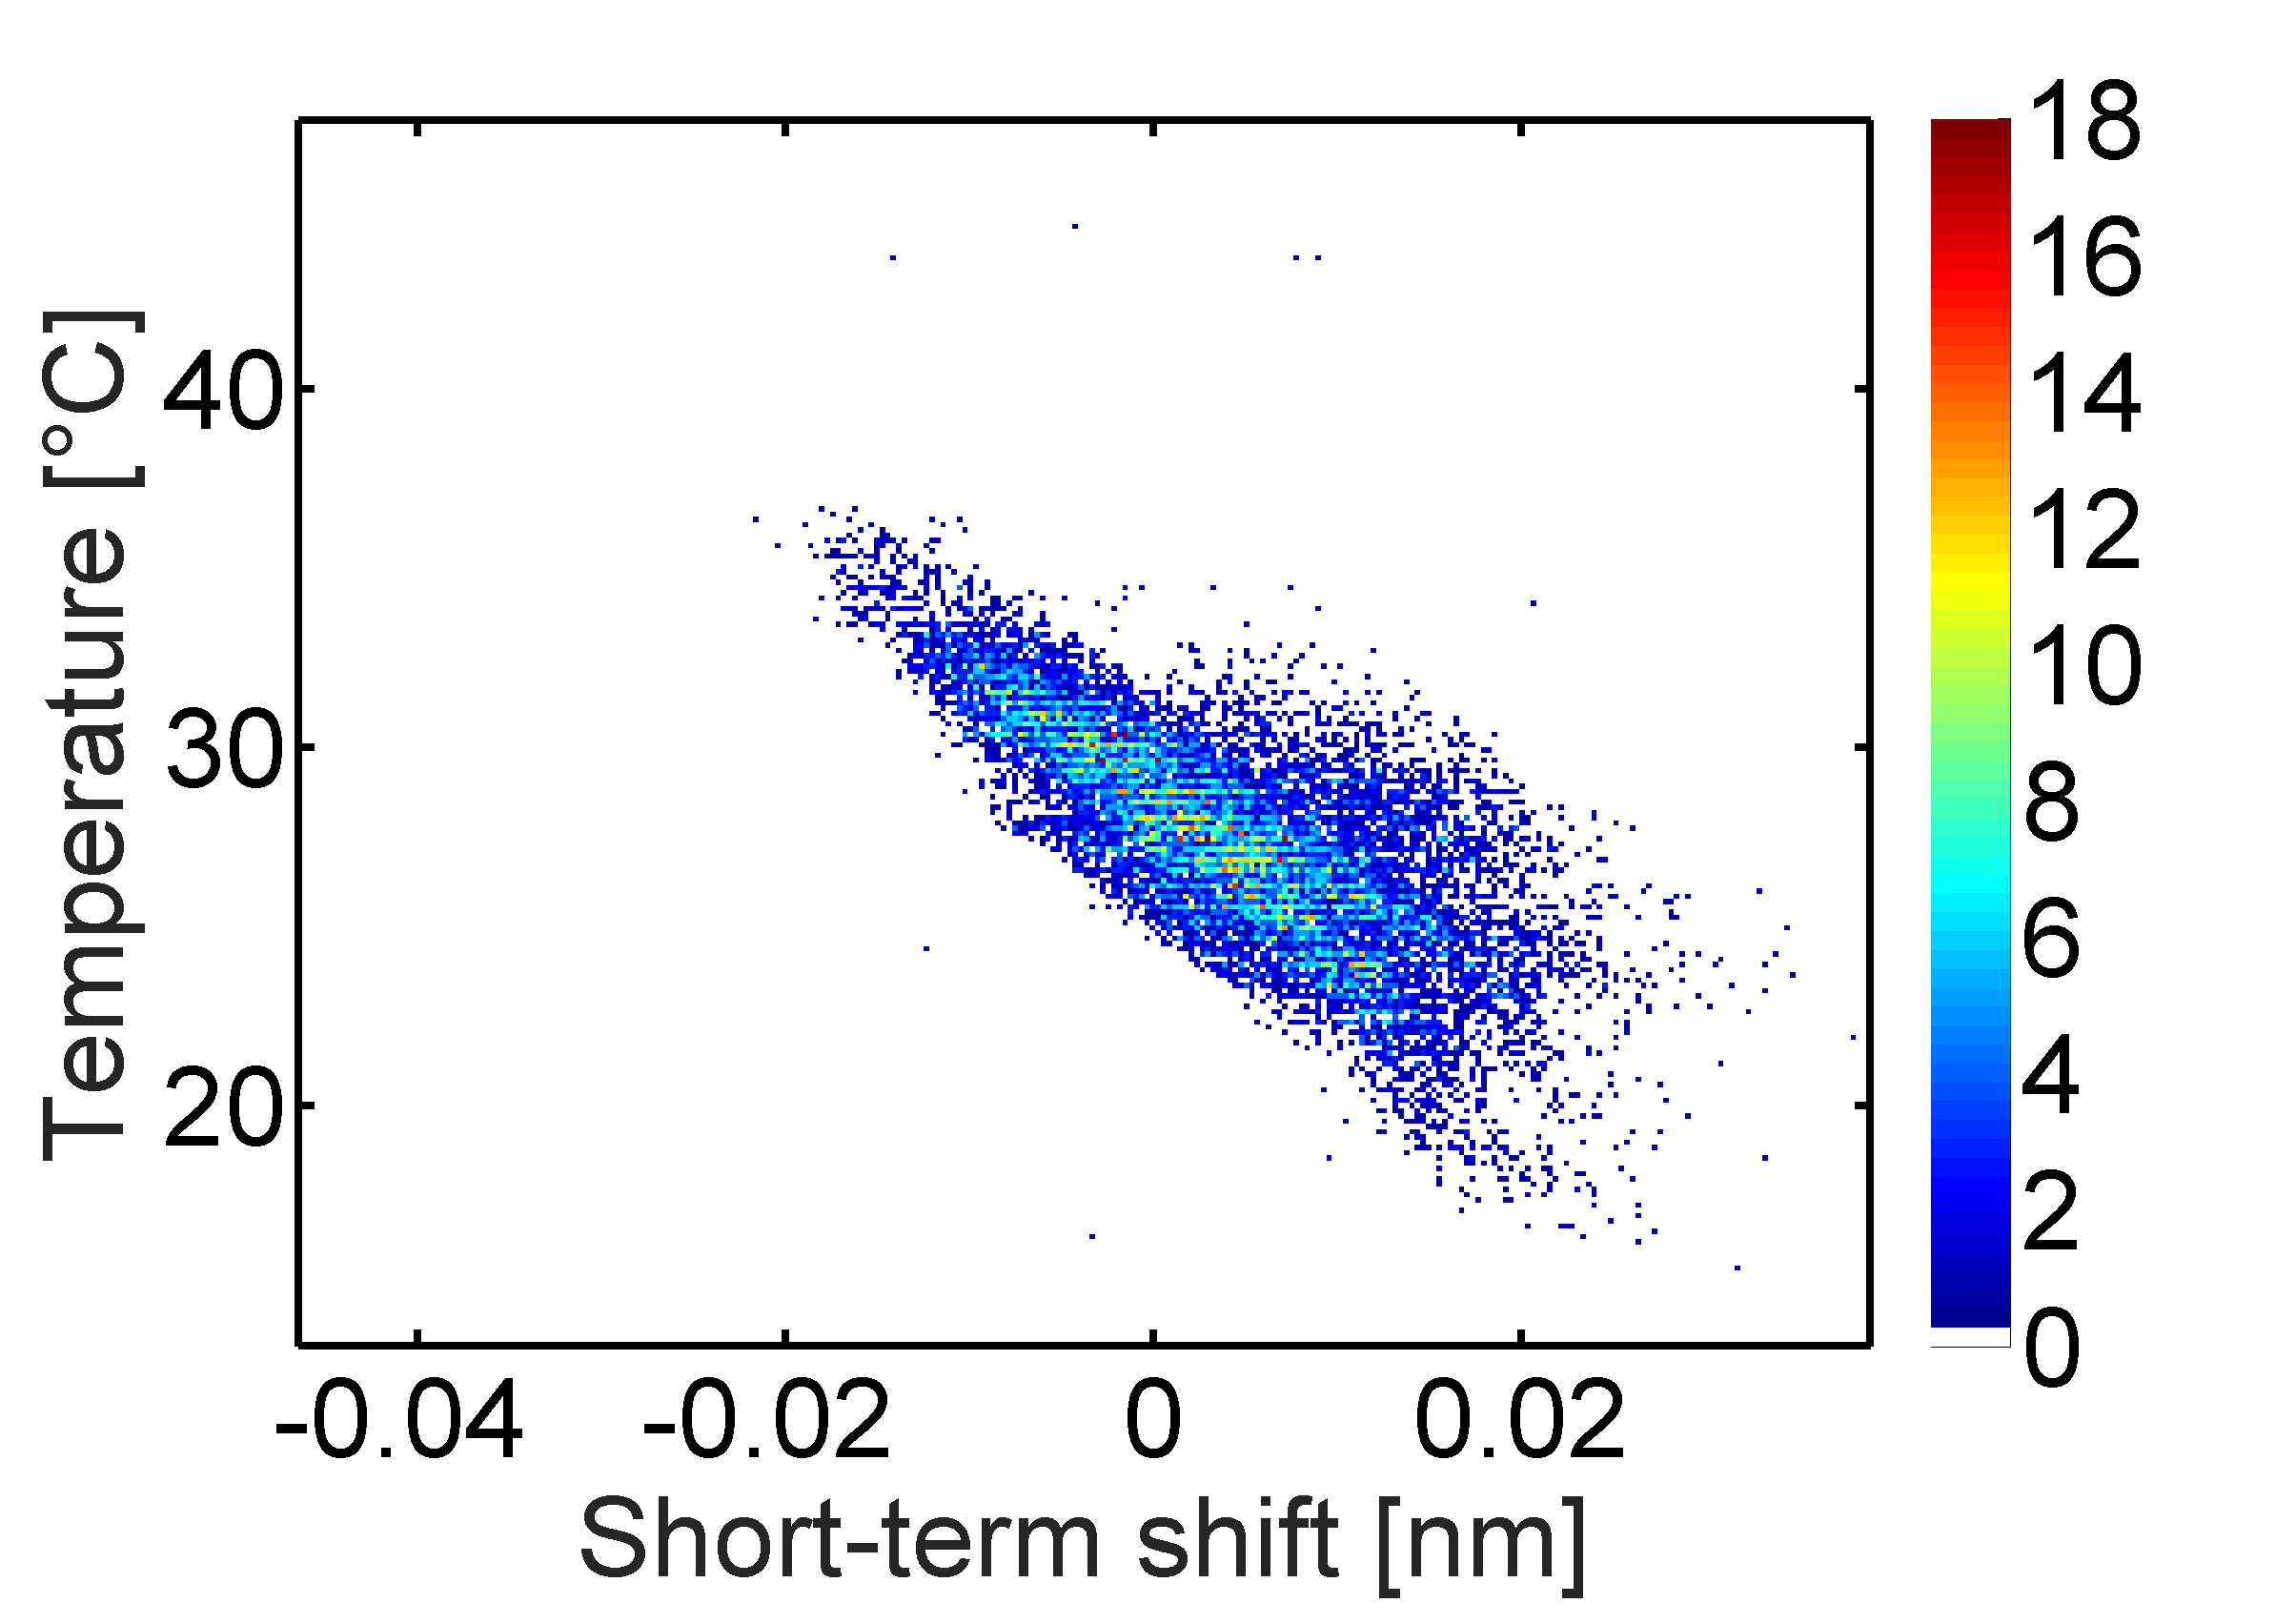
\includegraphics[width=0.49\textwidth]{Bilder/Simon/Bilder_Tung/D2J2140_After}}
		\caption{Short Term wavelength as a function of the instrument temperature for Pillate 1. (a) initial period  prior to January 2010 (b) after 2010. From \cite{WarnachSimon}}
		\label{fig:shorttermshift}
	\end{figure}
	

	\subsection{Temperature}
	\begin{figure}
		\subfigure[D2J2140\_0]{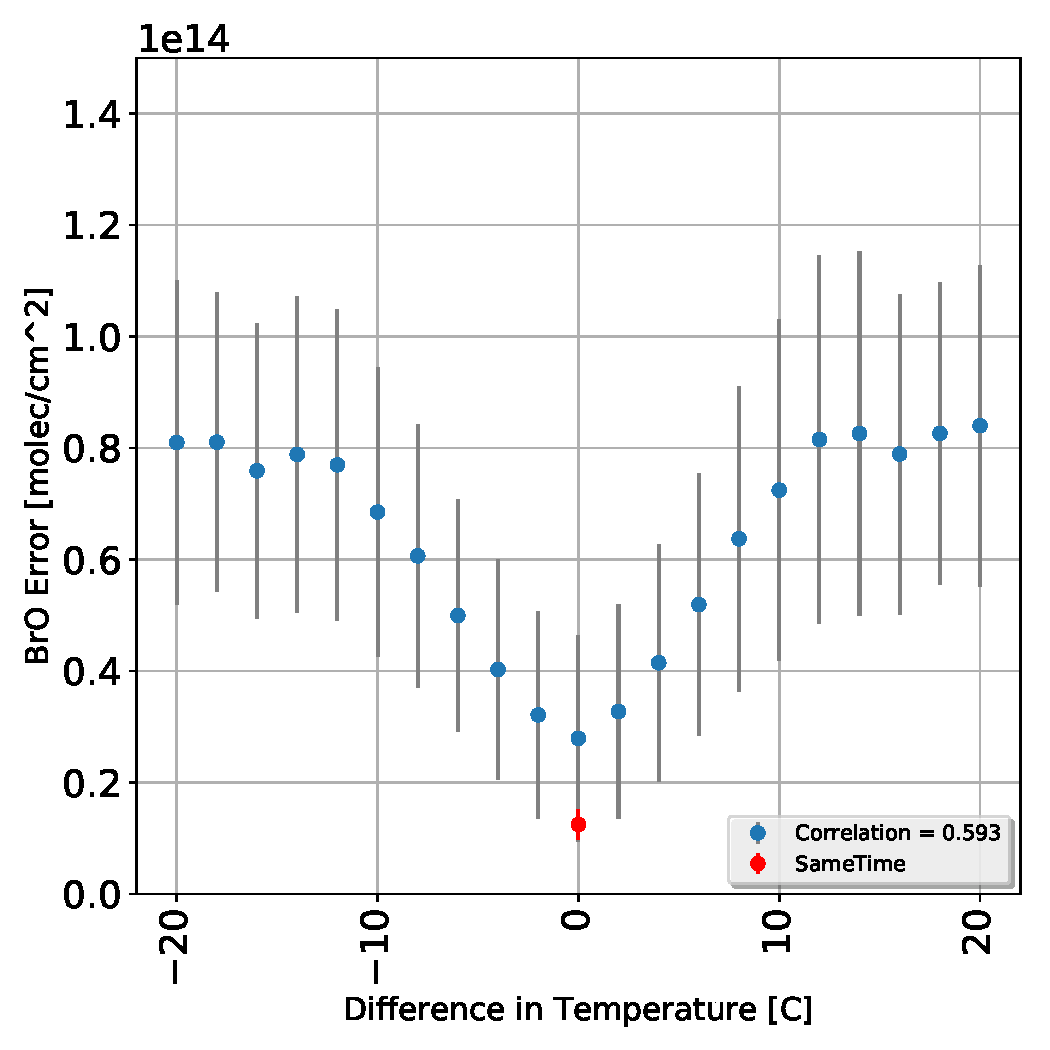
\includegraphics[width=0.3\linewidth]{Bilder/DEpendencoOfBrOErrorOnVariables_absolutedep/D2J2140_0BrOERR_DiffTemp_Tungu}}
		\subfigure[I2J8546\_0]{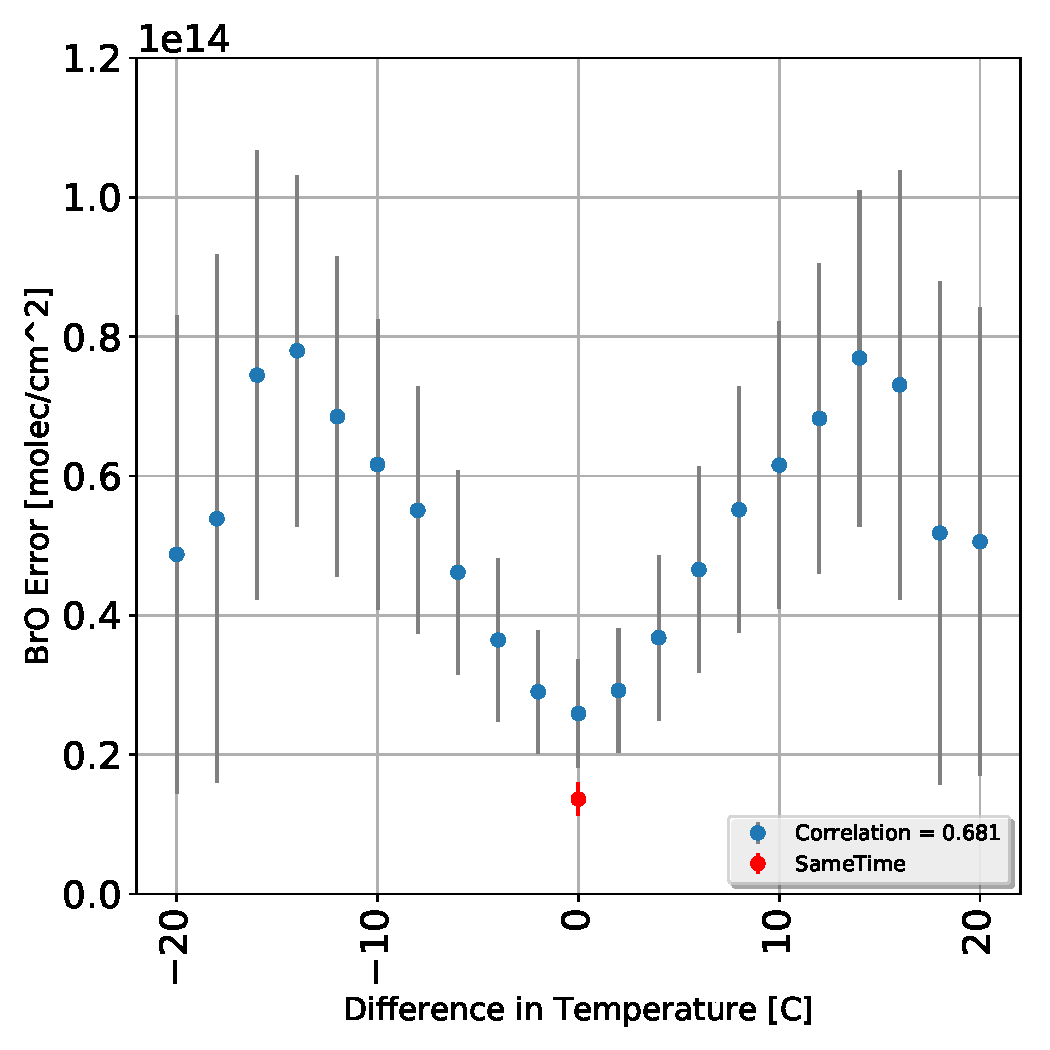
\includegraphics[width=0.3\linewidth]{Bilder/DEpendencoOfBrOErrorOnVariables_absolutedep/I2J8546_0BrOERR_DiffTemp_Tungu}}
		\subfigure[I2J8548\_0]{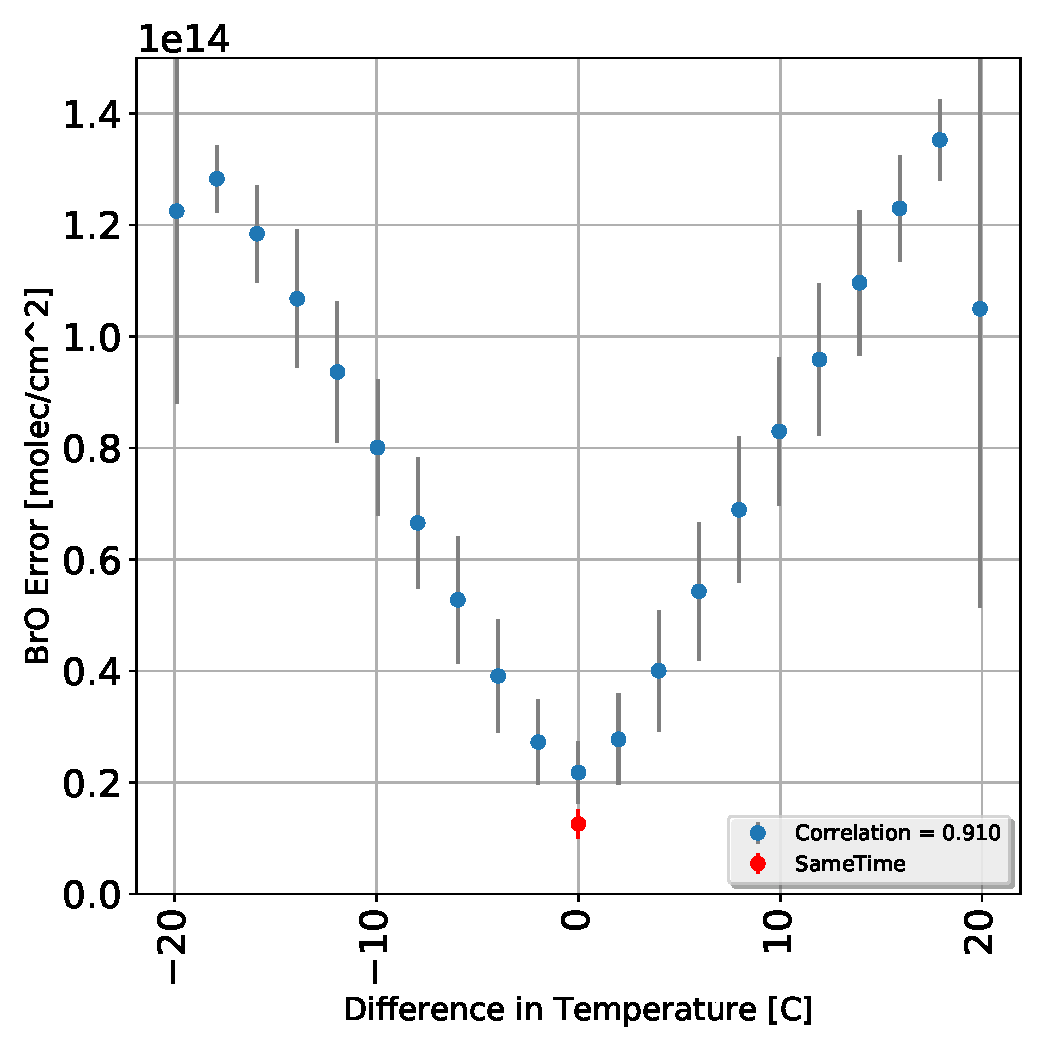
\includegraphics[width=0.3\linewidth]{Bilder/DEpendencoOfBrOErrorOnVariables_absolutedep/I2J8548_0BrOERR_DiffTemp_Tungu}}
		\centering
		\subfigure[]{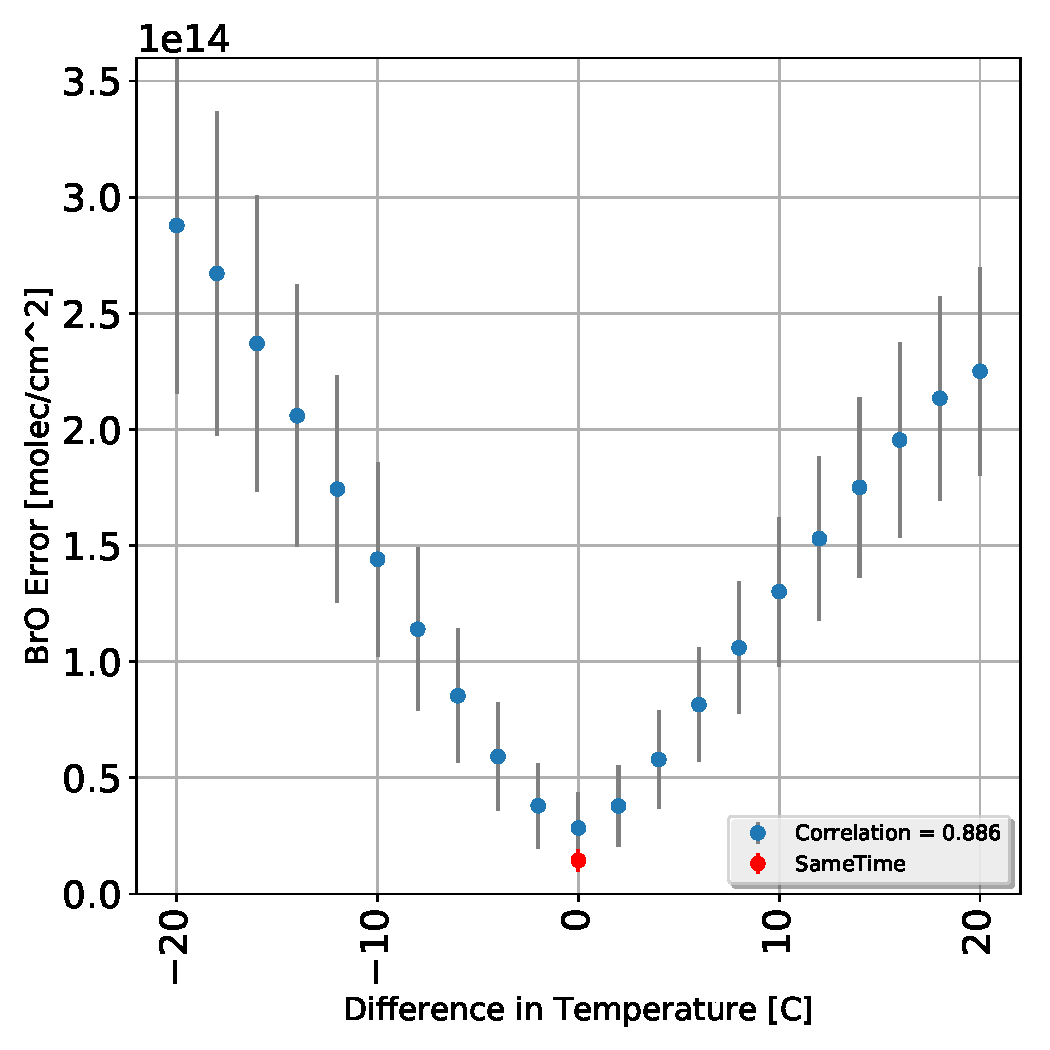
\includegraphics[width=0.3\linewidth]{Bilder/DEpendencoOfBrOErrorOnVariables_absolutedep/D2J2200_0BrOERR_DiffTemp_Nevad}}
		\subfigure[]{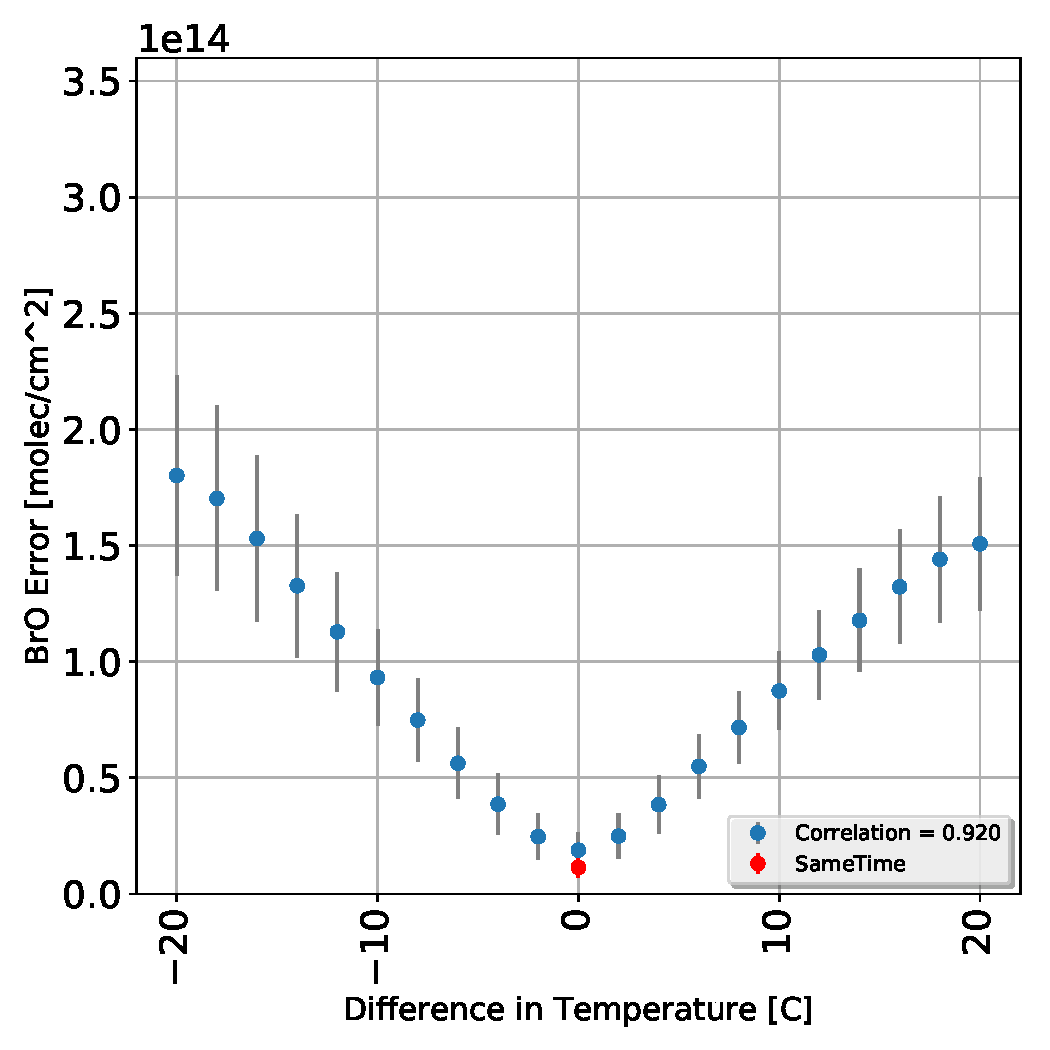
\includegraphics[width=0.3\linewidth]{Bilder/DEpendencoOfBrOErrorOnVariables_absolutedep/D2J2201_0BrOERR_DiffTemp_Nevad}}
		\caption{The BrO Measurement Error as a function of the difference of temperature between measuring the reference and the plume are shown. To evaluate the plume spectra all reference spectra with a temporal distance of no longer than two weeks are used. A increase of the BrO Error with the distance in temperature is observable.}
		\label{fig:difftemp}
	\end{figure}
	The instrument design of the NOVAC instruments compromise between accuracy and longetivity as explained in \cref{NOVAC}. In particular there are no internal thermal stabilizations installed as an attempt to reduce the need for power. This can influence the recorded spectra.\\	
	Each pixel of the spectrometer, which is used for the DOAS experiment, collects photons of a certain wavelength range.\\
	The calibration for the wavelength to pixel mapping (WMP) is commonly done with a Mercury lamp or by the comparison with the high defined Kuruz spectrum.
	As the WMP depends on the optical alignment of the spectrometer, which itself depends on the temperature, it is not constant.
	Changes in the spectrometers temperature can cause changes in the instrument line function and shifts in the WMP (\cite{pinardi2007influence}). 
	Moreover, \cite{WarnachSimon} show that, short term shifts are related to the instrument temperature (see \Cref{fig:shorttermshift}).\\
	The above discussed temperature dependence of the WMP causes a reduction of the fitquality with increasing instrument temperature difference between plume and reference. Thus the \ce{BrO} Error increases as well with the temperature difference. To quantify the \ce{BrO} error dependency on the temperature all plume spectra of Tungurahua from August 2008 to August 2009 (Nevado del Ruiz from end of 2009 to the end of 2011) where evaluated  with respect to all plume spectra of the same time period. 
	The \ce{BrO} error as function of the temperature difference can be seen in \cref{fig:difftemp}. The blue dots shows the mean \ce{BrO} error at the specific temperature difference, the standard deviation is illustrated with gray bars.\\
	The mean BrO deviation for the sametime evaluation is additionally added with a red point.
	\begin{itemize}
		\item The BrO error as a function of the difference in temperature is symmetric around zero for all observed instruments, thus the absolute difference in temperature is sufficient when evaluating the dependence on the temperature.
		\item The BrO error show a large (up to 0.92 at D2J2201\_0 (\cref{fig:difftemp} (e))) correlation with the temperature difference.
		\item The dependence on the temperature changes for every instrument.
		\item The \ce{BrO} error has the strongest dependence on the temperature difference. 
	\end{itemize}
	
	\begin{align*}
		\rightarrow&  BrO_{Error} = f(ext. P)+ 3.53\cdot10^{12}\cdot\frac{\Delta T}{1C^{\circ}} + \mathcal{O}\left(\right) & Tungurahua\\
		\rightarrow&  BrO_{Error} = f(ext. P)+7.56\cdot10^{12}\cdot\frac{\Delta T}{1C^{\circ}} + \mathcal{O}\left(\right) & Nevado Del Ruiz\\
	\end{align*}


	\begin{table}[h]
		\begin{tabular}{|p{2cm}|p{2cm}|p{2cm}|p{2cm}|p{2cm}|p{2cm}|}
			%	\toprule
		Instrument	&D2J2140\_0&I2J8546\_0& I2J8548\_0&D2J2200\_0&D2J2201\_0\\
			\toprule
			Slope&4.10e+12 &3.93e+12 &6.50e+12 &1.24e+13&8.17e+12 \\
			\midrule
			Correlation
			& 
			0.593& 
			0.681& 
			0.910& 
			0.886& 
			0.920\\
			\midrule
			Zero point&2.58e+13&2.23e+13&1.60e+13& 1.38e+13& 9.07e+12\\
			\bottomrule
		\end{tabular}
	\end{table}
	When looking at all discussed external parameters, temperature has  the strongest impact on the \ce{BrO} error due to the strong impact on the WMP.
	\subsection{Daytime \label{chap:daytime}}
	\begin{figure}
		\subfigure[]{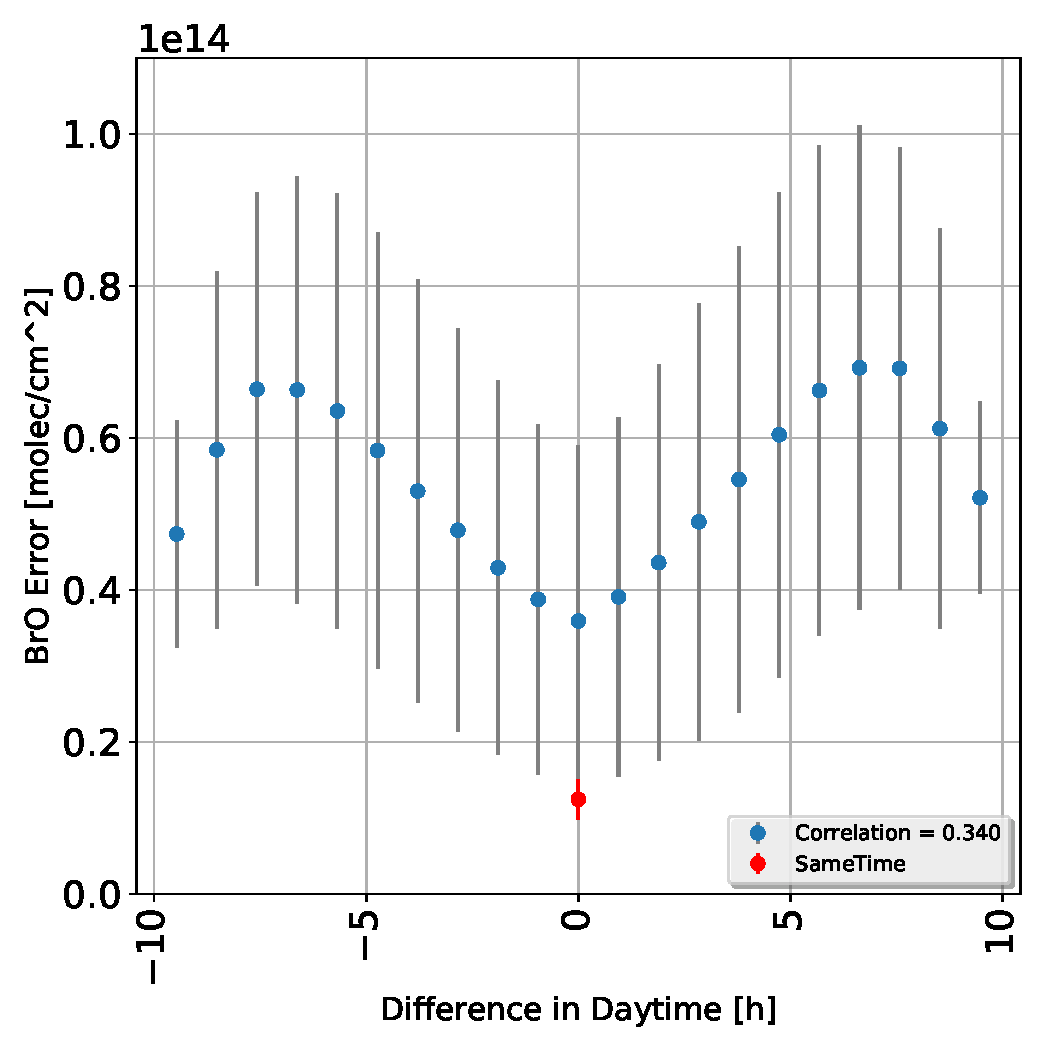
\includegraphics[width=0.3\linewidth]{Bilder/DEpendencoOfBrOErrorOnVariables_absolutedep/D2J2140_0BrOERR_DiffDaytime_Tungu}}
		\subfigure[]{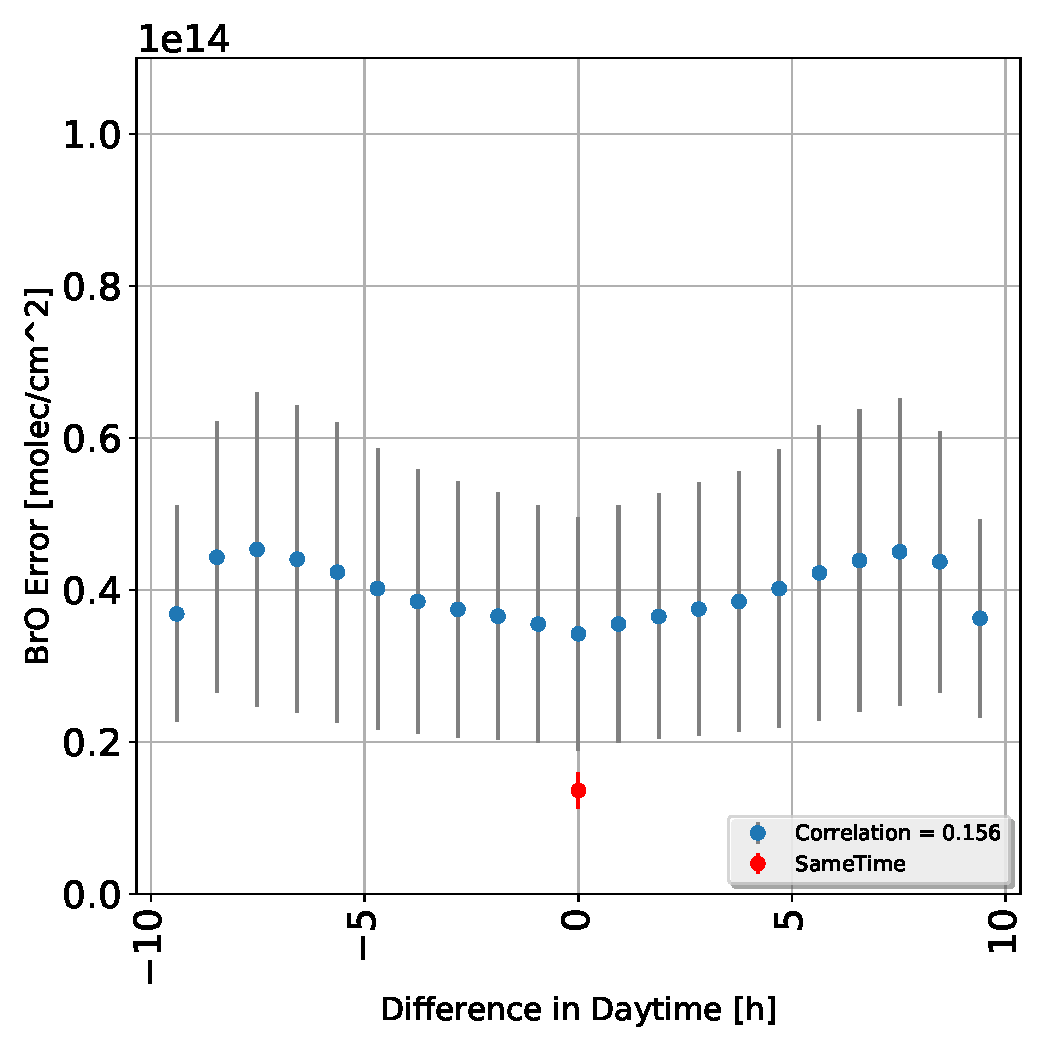
\includegraphics[width=0.3\linewidth]{Bilder/DEpendencoOfBrOErrorOnVariables_absolutedep/I2J8546_0BrOERR_DiffDaytime_Tungu}}
		\subfigure[]{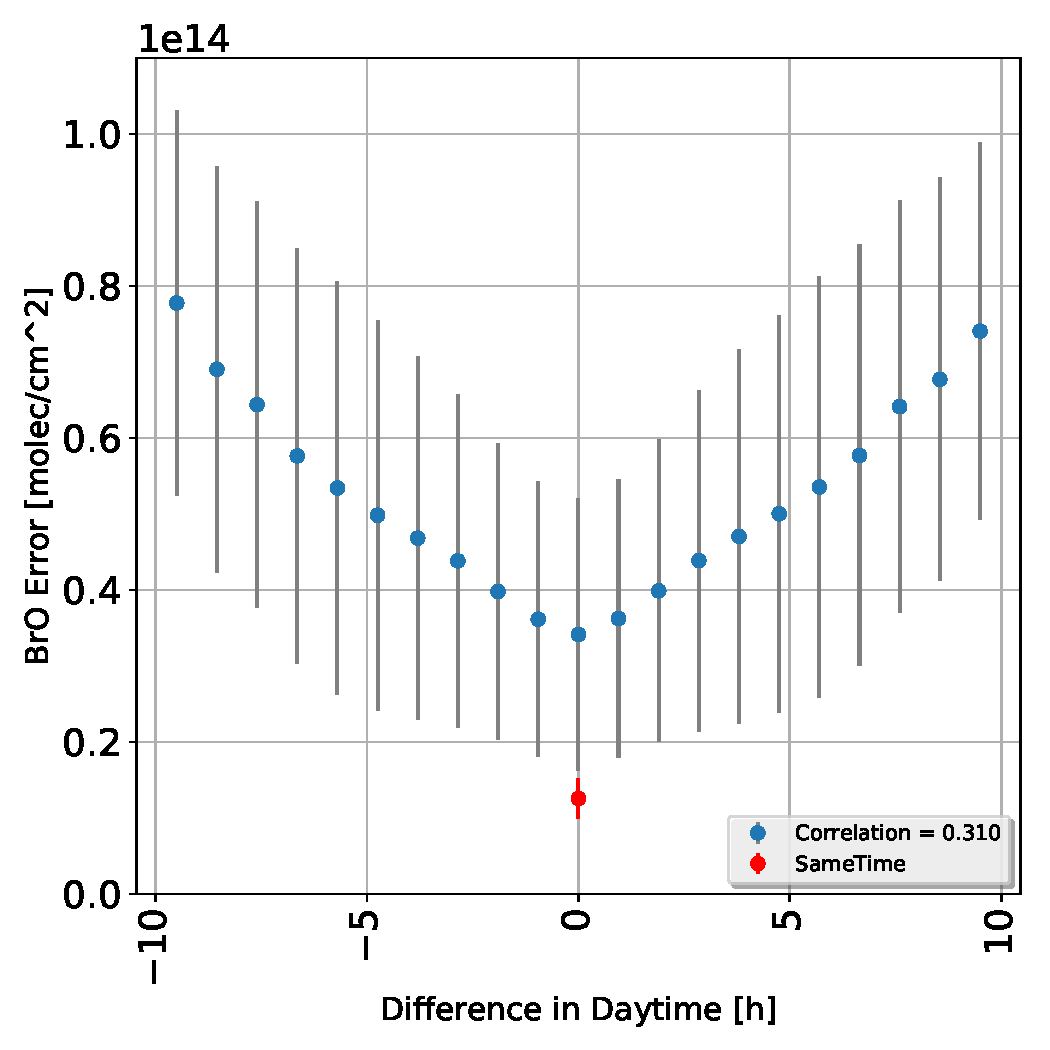
\includegraphics[width=0.3\linewidth]{Bilder/DEpendencoOfBrOErrorOnVariables_absolutedep/I2J8548_0BrOERR_DiffDaytime_Tungu}}
		\centering
		\subfigure[]{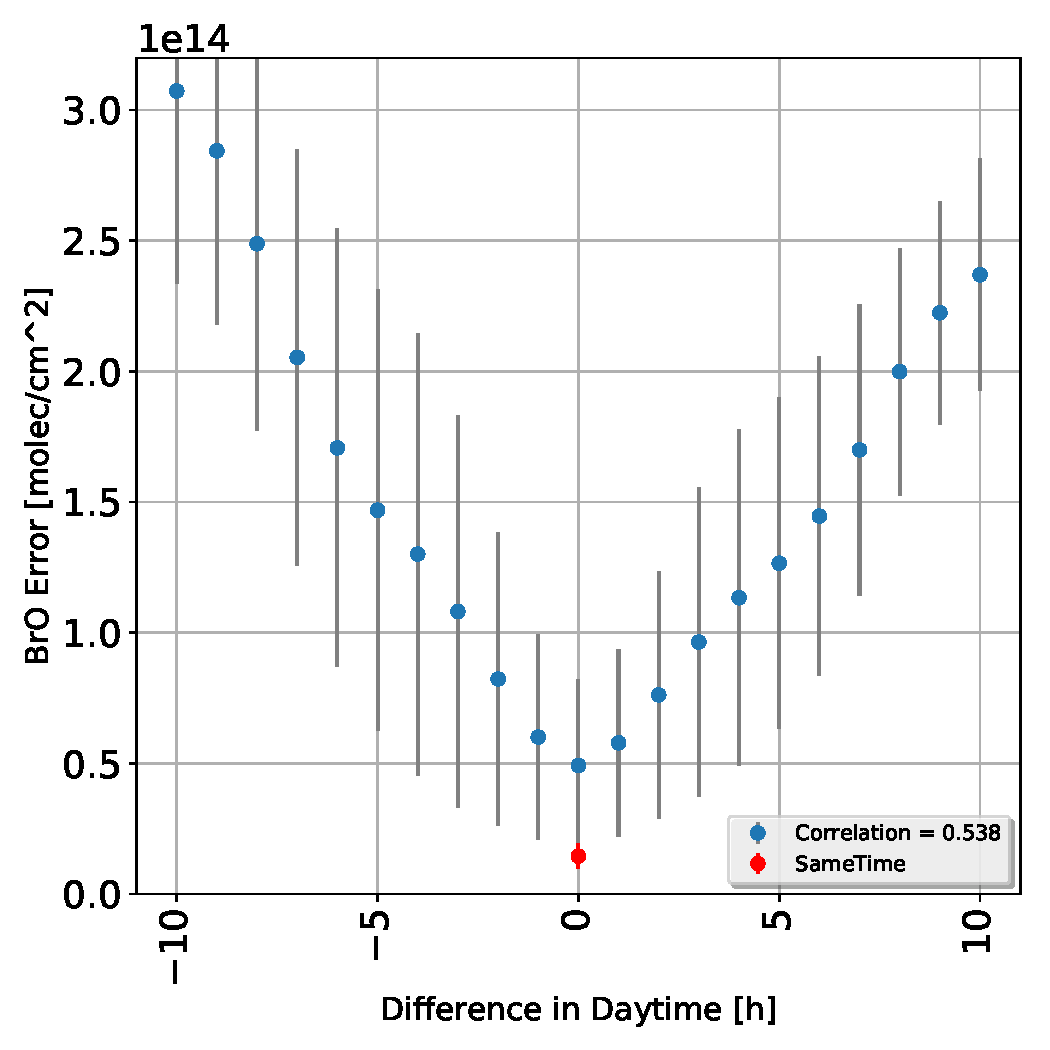
\includegraphics[width=0.3\linewidth]{Bilder/DEpendencoOfBrOErrorOnVariables_absolutedep/D2J2200_0BrOERR_DiffDaytime_Nevad}}
		\subfigure[]{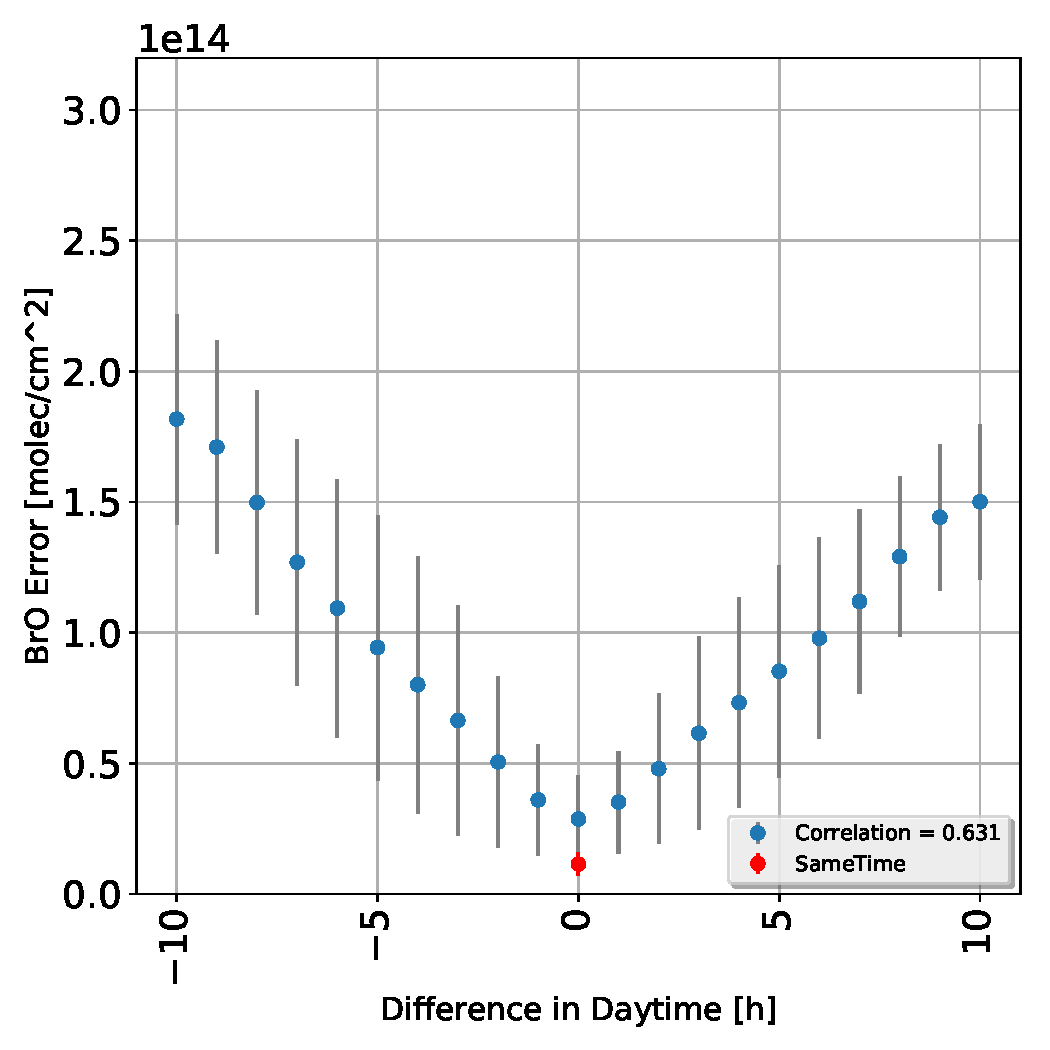
\includegraphics[width=0.3\linewidth]{Bilder/DEpendencoOfBrOErrorOnVariables_absolutedep/D2J2201_0BrOERR_DiffDaytime_Nevad}}
		\caption{The BrO Measurement Error as a function of the difference of the day time between measuring the reference and the plume are shown. To evaluate the plume spectra all reference spectra with a temporal distance of no longer than two weeks are used. A increase of the BrO Error with the distance in day time is observable.}
		\label{fig:diffdaytime}
	\end{figure}
	During the day o al lot of external parameters like temperature, solar altitude etc. change. In particular the solar altitude could have an impact on the fit quality since the light path of the sun is much longer at the evening than at noon. Therefore the scattering effects and the fraunehofer structures is different for both spectra.\\
	\Cref{fig:diffdaytime} shows the dependency of the \ce{BrO} error on the daytime. The data are calculated as described for the temperature. 
	
	\begin{itemize}
		\item The BrO error as a function of the difference in daytime is almost symmetric around zero for all observed instruments, thus the absolute difference in temperature is sufficient as well when evaluating the dependence on the daytime.
		\item The correlations of the instruments at the Nevado Del Ruiz volcano are significantly higher than at Tungurahua. The strongest correlation can be seen at Nevado Del Ruiz at D2J2201\_0 with 0.631 (e)
		\item The I2J8546\_0 instrument does not show any significantly correlation
		\item For very large daytime difference a decrease of the BrO error can be observed at D2J2140\_0.
	\end{itemize}
		\begin{align*}
		\rightarrow&  BrO_{Error} = f(ext. P)+1.33\cdot10^{12}\cdot\frac{\Delta DT}{1h}  + \mathcal{O}\left(\right)& Tungurahua\\
		\rightarrow&  BrO_{Error} = f(ext. P)+1.58\cdot10^{13}\cdot\frac{\Delta DT}{1h} + \mathcal{O}\left(\right) & Nevado Del Ruiz\\
		\end{align*}

	\begin{table}[h]
		\begin{tabular}{|p{2cm}|p{2cm}|p{2cm}|p{2cm}|p{2cm}|p{2cm}|}
			%	\toprule
			Instrument	&D2J2140\_0&I2J8546\_0& I2J8548\_0&D2J2200\_0&D2J2201\_0\\
			\toprule
			Slope&5.07e+12&1.40e+12 &3.77e+12 &2.04e+13& 1.38e+13\\
			\midrule
			Correlation&
			0.340&
			0.156&
			0.310&
			0.538&
			0.631\\
			\midrule
			Zero point& 3.43e+13&3.39e+13&3.28e+13&  4.01e+13&  2.24e+13\\
			\bottomrule
		\end{tabular}
	\end{table}
	\subsection{Colorindex}
	\begin{figure}
		\subfigure[]{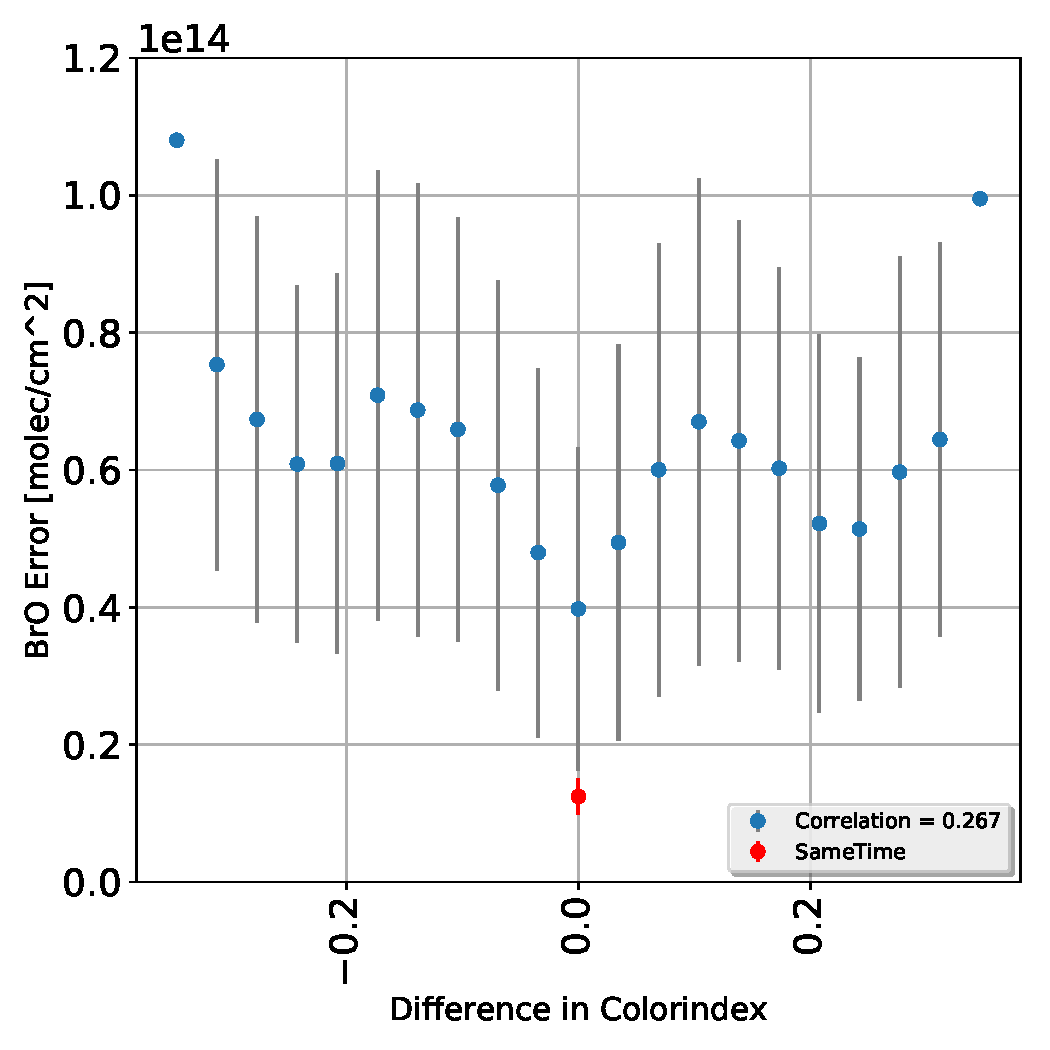
\includegraphics[width=0.3\linewidth]{Bilder/DEpendencoOfBrOErrorOnVariables_absolutedep/D2J2140_0BrOERR_DiffColidx_Tungu}}
		\subfigure[]{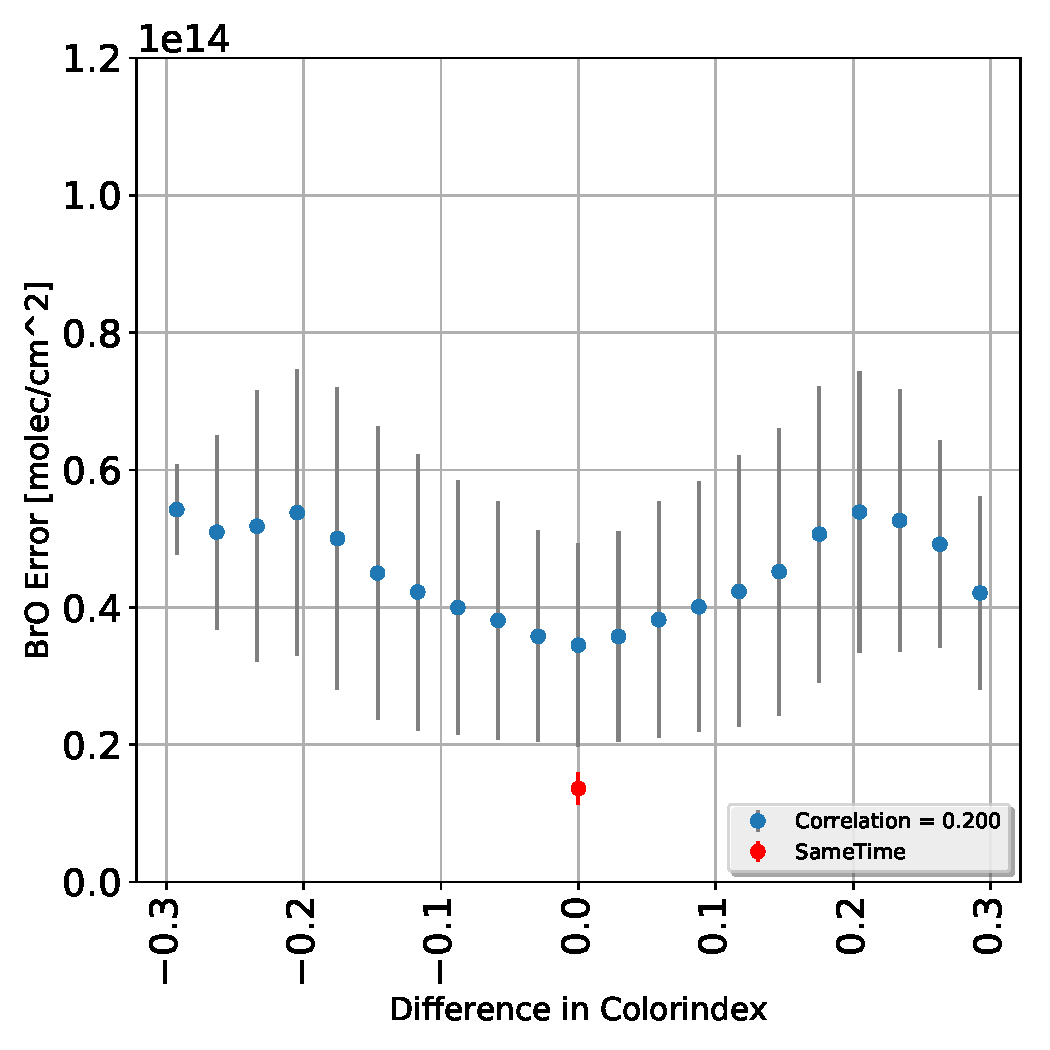
\includegraphics[width=0.3\linewidth]{Bilder/DEpendencoOfBrOErrorOnVariables_absolutedep/I2J8546_0BrOERR_DiffColidx_Tungu}}
		\subfigure[]{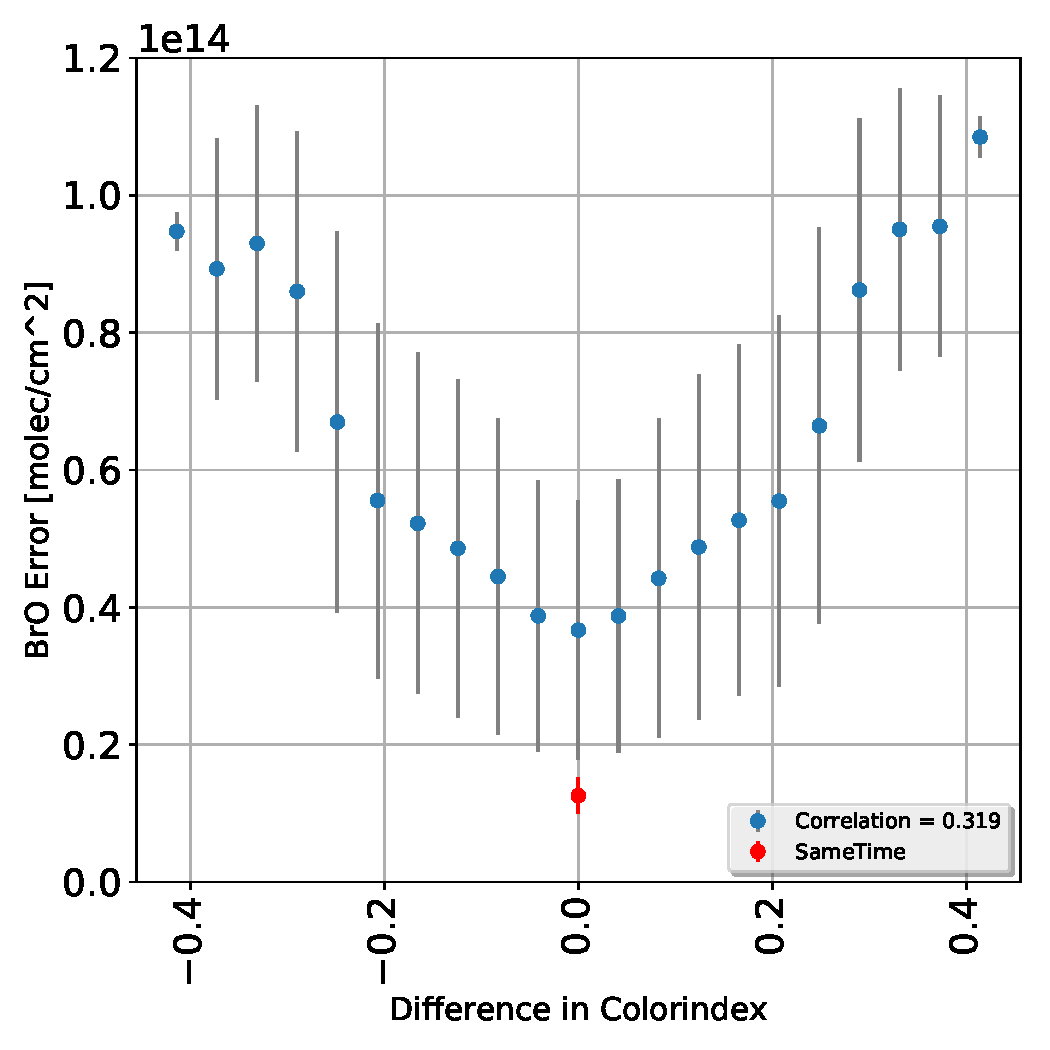
\includegraphics[width=0.3\linewidth]{Bilder/DEpendencoOfBrOErrorOnVariables_absolutedep/I2J8548_0BrOERR_DiffColidx_Tungu}}
		\centering
		\subfigure[]{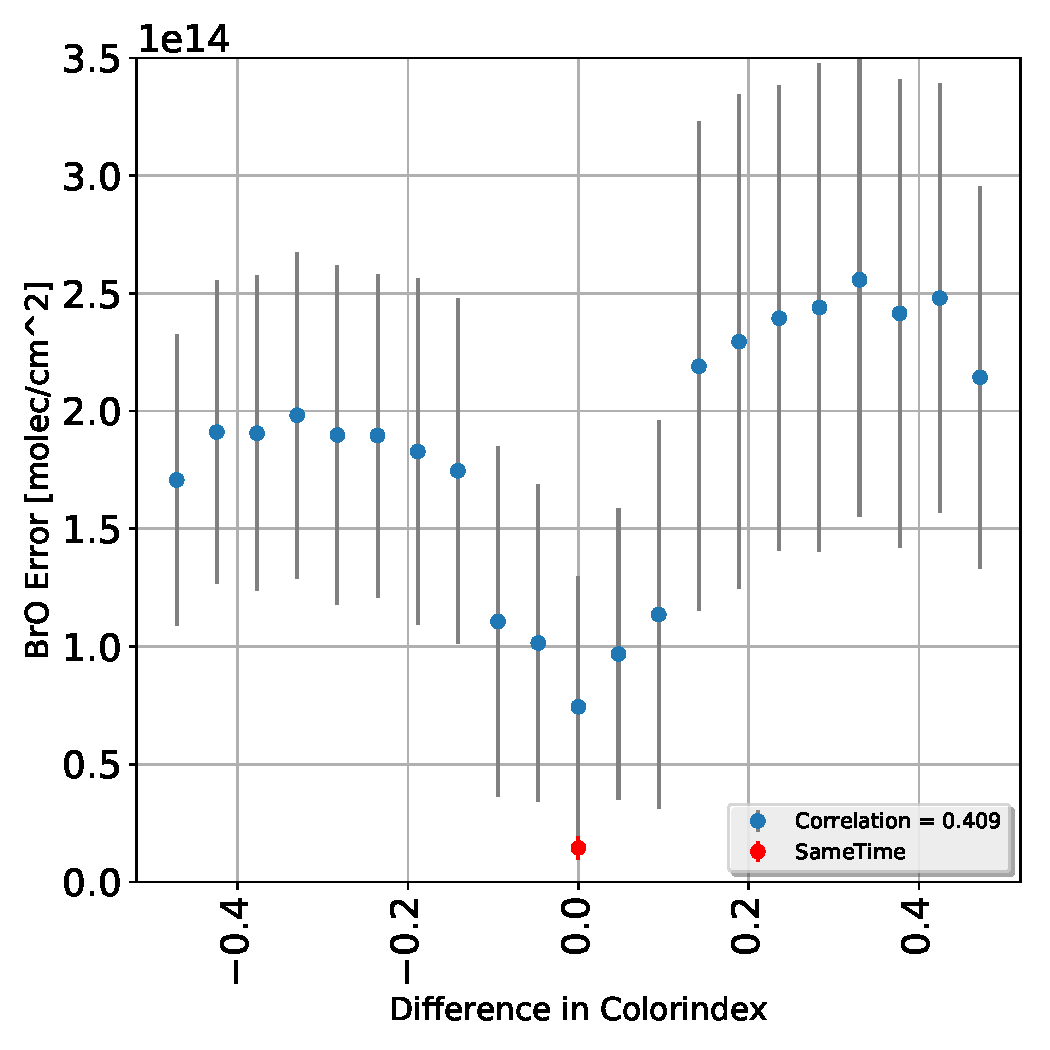
\includegraphics[width=0.3\linewidth]{Bilder/DEpendencoOfBrOErrorOnVariables_absolutedep/D2J2200_0BrOERR_DiffColidx_Nevad}}
		\subfigure[]{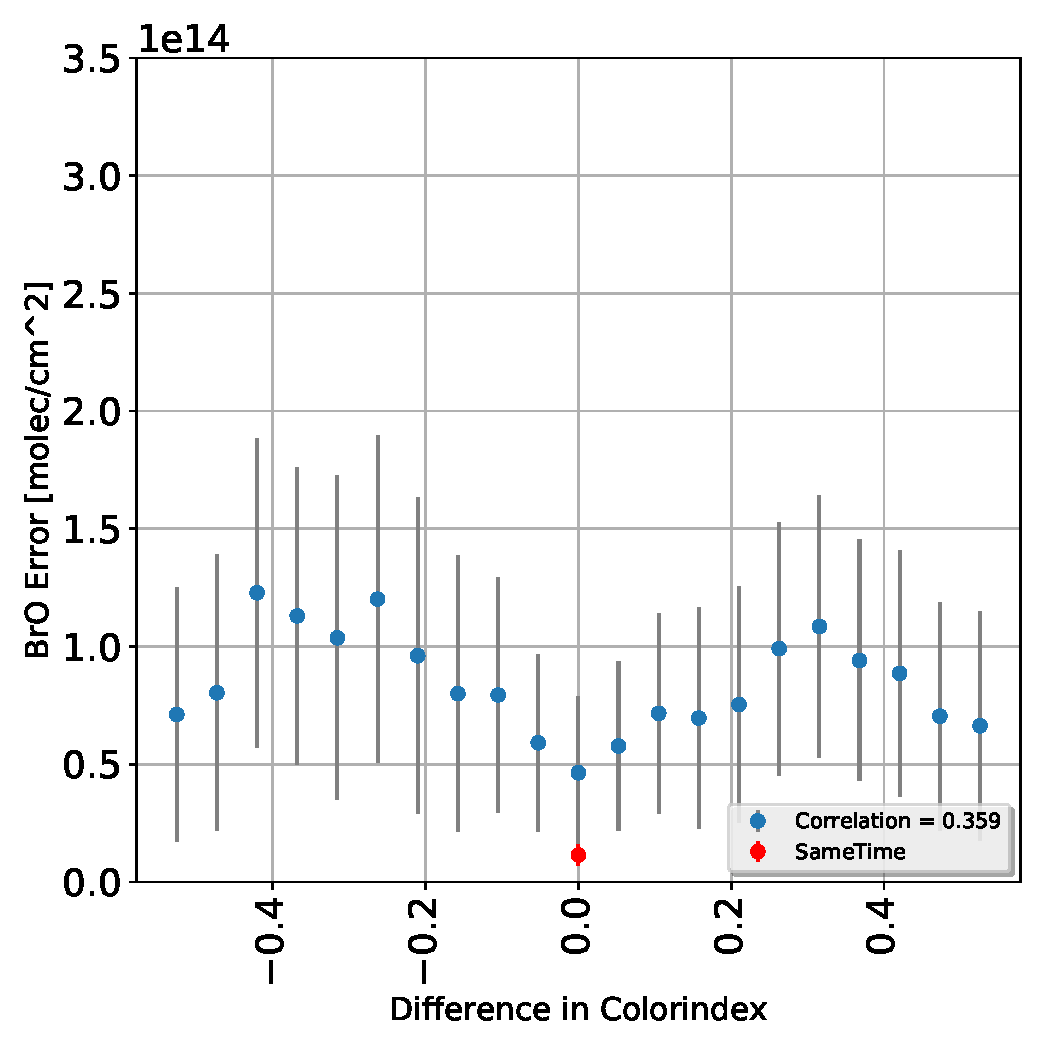
\includegraphics[width=0.3\linewidth]{Bilder/DEpendencoOfBrOErrorOnVariables_absolutedep/D2J2201_0BrOERR_DiffColidx_Nevad}}
		\caption{The BrO Measurement Error as a function of the difference of colorindex between measuring the reference and the plume are shown. To evaluate the plume spectra all reference spectra with a temporal distance of no longer than two weeks are used. A increase of the BrO Error with the distance in colorindex is observably.}
		\label{fig:diffcolidx}
	\end{figure}

	Clouds  have  a  strong  influence  on  the  atmospheric  radiative  transfer  and  thus  affect  the  interpretation  and  analysis of DOAS - observations \cite{wagner2014cloud}.
	
	Clouds can be identified by several measurement quantities that they influence.
	As Mie scattering is dominant in clouds the wavelength of the light that is scattered is different than the Rayleigh sky. Thus, clouds can be easily identified by their white color.
	Therefore, the cloudiness of the sky can be quantified in a scalar measure defined by the ratio of the measured intensity at two wavelengths, the so-called colour index.
	\cite{wagner2014cloud} showed that for a zenith-looking instrument the measured radiation intensity is enhanced by clouds. Thus, clouds can cause large errors for the retrieved gas column density and the corresponding uncertainties. 
	Cloud effects are especially severe if the cloudiness for the recorded plume and reference spectra strongly defer. Also for broken clouds the described effect can be observed as measurements at some elevation angles might be influenced by clouds while others are not.
	In this work the Colour Index (CI) is the ratio between the intensities at 320nm and 360 nm.
	These two wavelengths are as far apart as the filter used for stray-light prevention in the spectrometers allows.
	%% I don’t understand 	
	On the other hand, the lower wavelength avoids the deep UV range where \ce{SO2} and O3 absorption plays a dominant role.
	%% I don’t understand 	
	The Mie scattering in the clouds is responsible for the higher amount of radiation from larger wavelengths. This results in a decrease of the CI (\cite{lubcke2014optical}).
	\\
	We evaluated the CI at the zenith, to increase the stability of the fit we added in each cases 10 intensitys. Using always the zenith to evaluate the colour index makes the colour index more comparable, but if broken clouds occur, the CI of the reference and the plume could differ from the calculated CI of the zenith. This could be a reason for the large deviations of the mean \ce{BrO} error as function of the colour index (see \cref{fig:diffcolidx})
	\begin{itemize}
		\item The BrO error as a function of the difference in colour index is also symmetric around zero for all observed instruments, thus the absolute difference in colour index is sufficient for the evaluating.
		\item The BrO error decreases for extreme differences in colour index for almost all instruments, the only exception is the  I2J8548\_0 at Tungurahua. Especially at D2J2140\_0 the curve is not monotonically increasing with increasing difference in colorindex. Even though  D2J2140\_0 is symmetric around zero.
	\end{itemize}
	\begin{itemize}
		\item 	The \ce{BrO} Error increases with the Colorindex differences as \\
		\begin{align*}
		\rightarrow&  BrO_{Error} = f(ext. P)+ 1.01\cdot10^{13}\cdot\frac{\Delta Cidx}{0.1} + \mathcal{O}\left(\right) & Tungurahua\\
		\rightarrow&  BrO_{Error} = f(ext. P)+  4\cdot10^{13}\cdot\frac{\Delta Cidx}{0.1} + \mathcal{O}\left(\right) & Nevado Del Ruiz\\
		\end{align*}
	\end{itemize}
	\begin{table}[h]
	\begin{tabular}{|p{2cm}|p{2cm}|p{2cm}|p{2cm}|p{2cm}|p{2cm}|}
			%	\toprule
			Instrument	&D2J2140\_0&I2J8546\_0& I2J8548\_0&D2J2200\_0&D2J2201\_0\\
			\toprule
			Slope&2.30e+14 &7.92e+13 &1.17e+14 &5.42e+14&1.91e+14\\
			\midrule
			Correlation&
			0.267&
			0.200&
			0.319&
			0.409&
			0.359\\
			\midrule
			Zero point&4.01e+13&3.36e+13&3.47e+13& 7.21e+13& 4.74e+13\\
			\bottomrule
		\end{tabular}
	\end{table}
		\subsection{Elevation Angle}
	\begin{figure}
		\subfigure[]{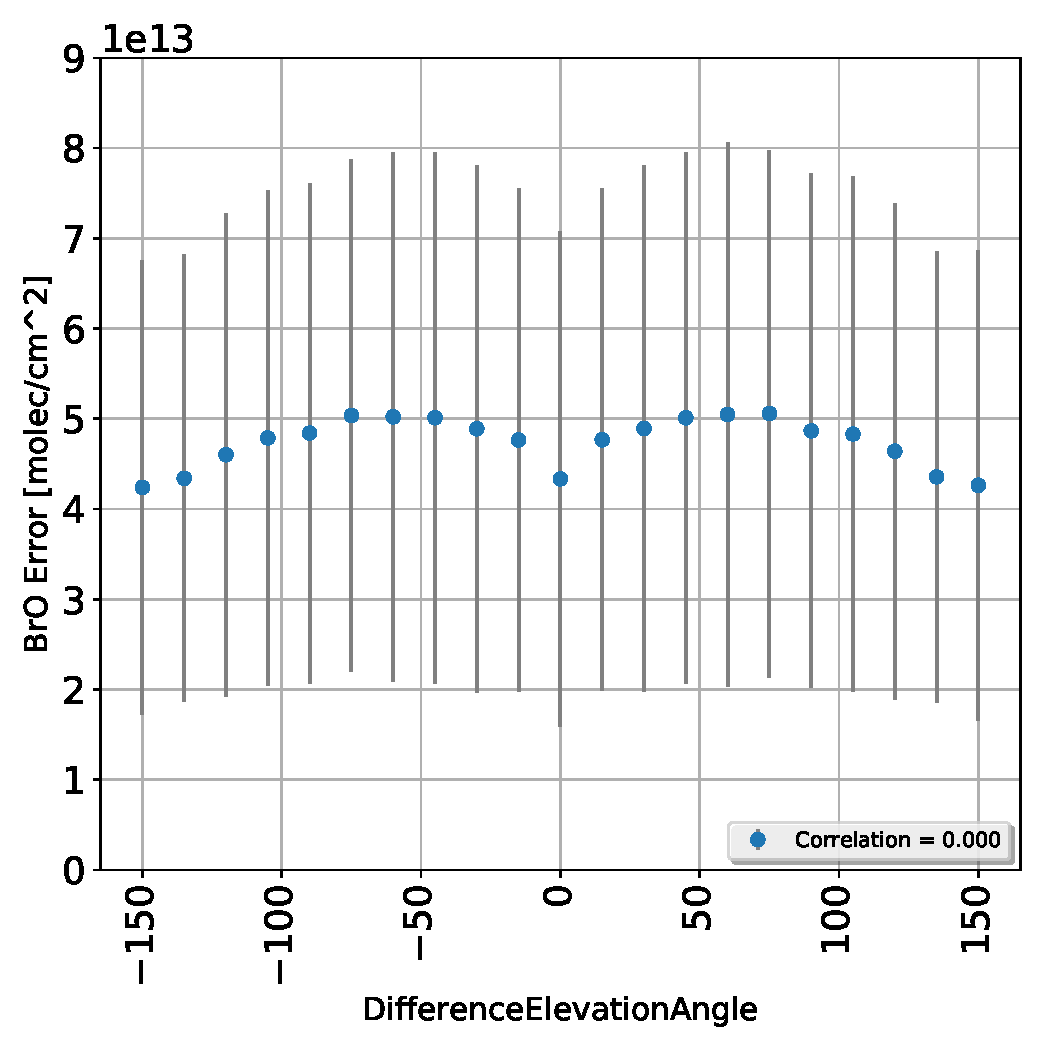
\includegraphics[width=0.3\linewidth]{Bilder/DEpendencoOfBrOErrorOnVariables_absolutedep/D2J2140_0BrOERR_DiffElevAngle_Tungu}}
		\subfigure[]{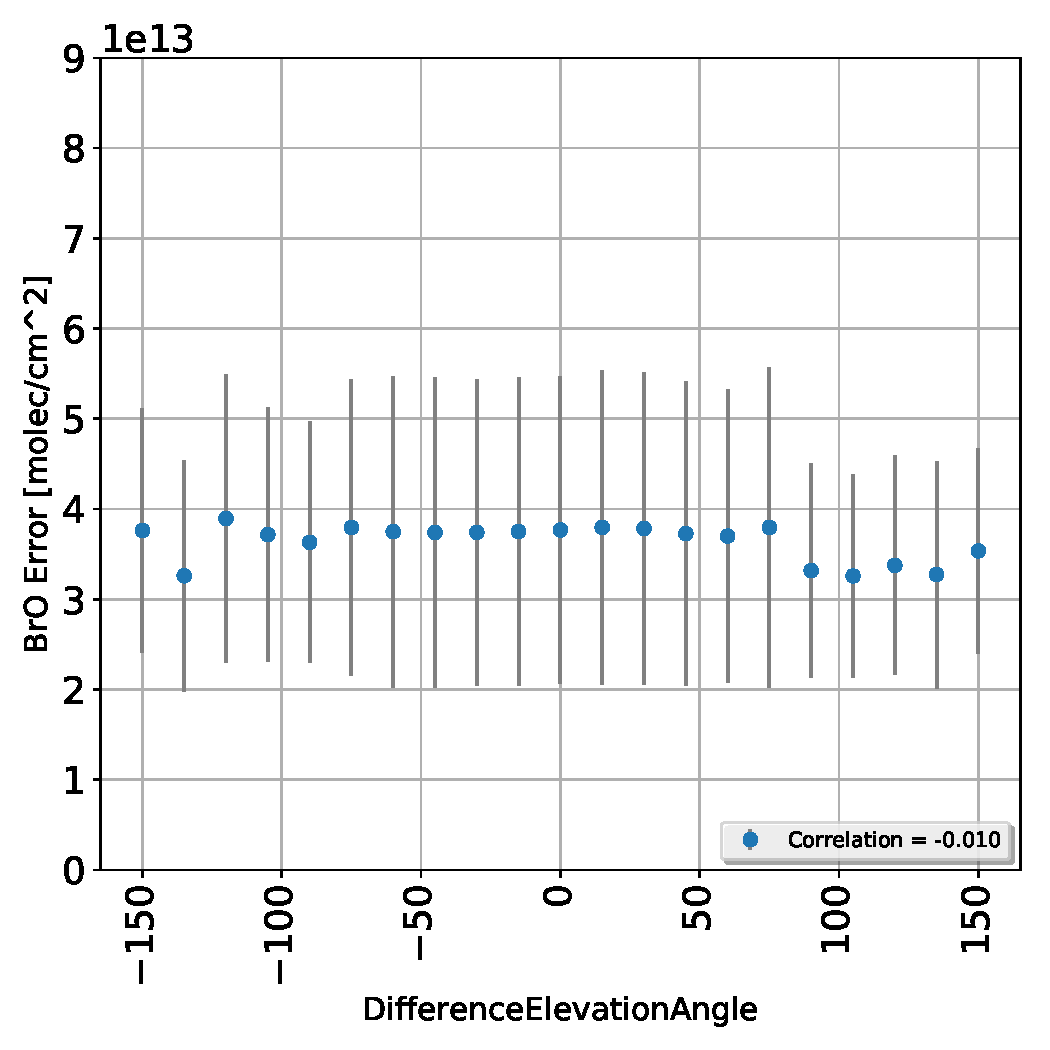
\includegraphics[width=0.3\linewidth]{Bilder/DEpendencoOfBrOErrorOnVariables_absolutedep/I2J8546_0BrOERR_DiffElevAngle_Tungu}}
		\subfigure[]{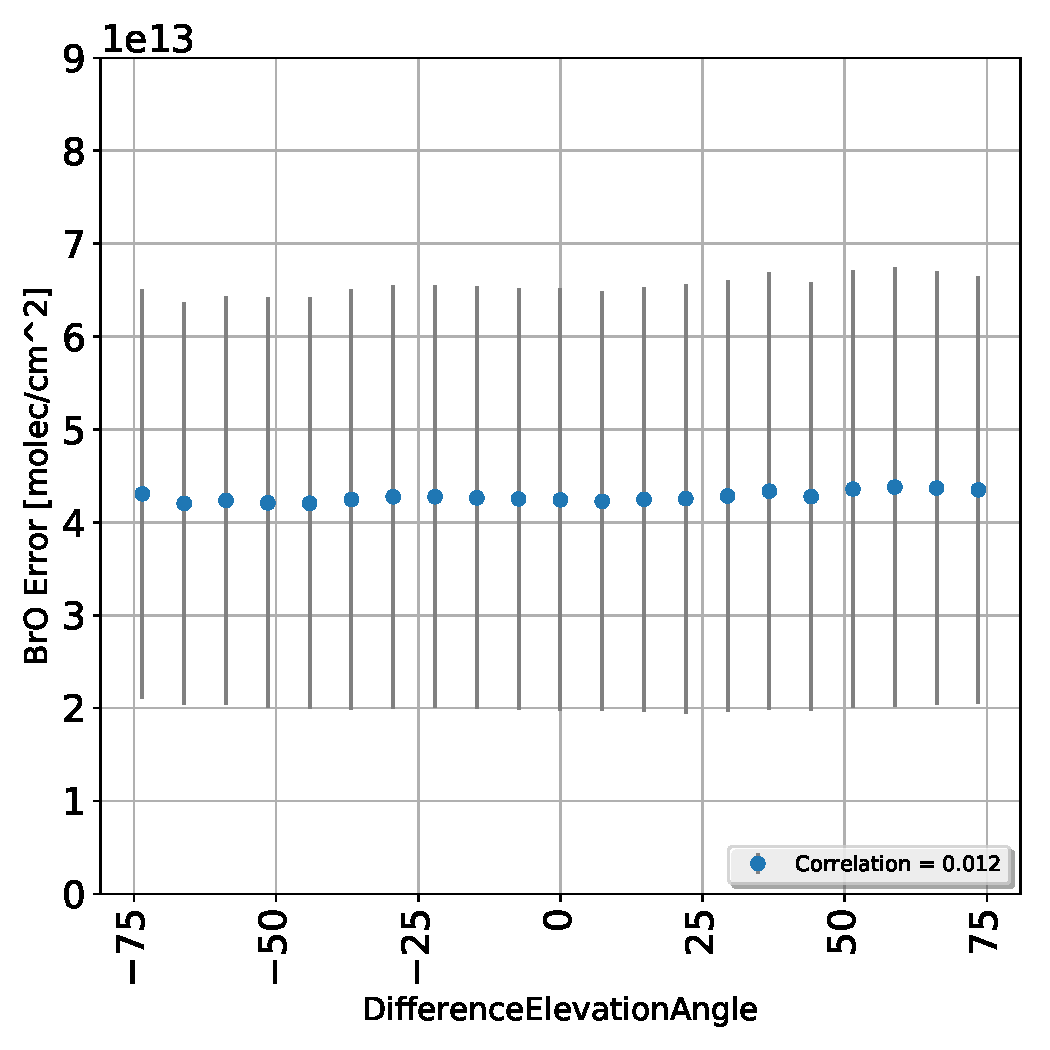
\includegraphics[width=0.3\linewidth]{Bilder/DEpendencoOfBrOErrorOnVariables_absolutedep/I2J8548_0BrOERR_DiffElevAngle_Tungu}}
		\centering
		\subfigure[]{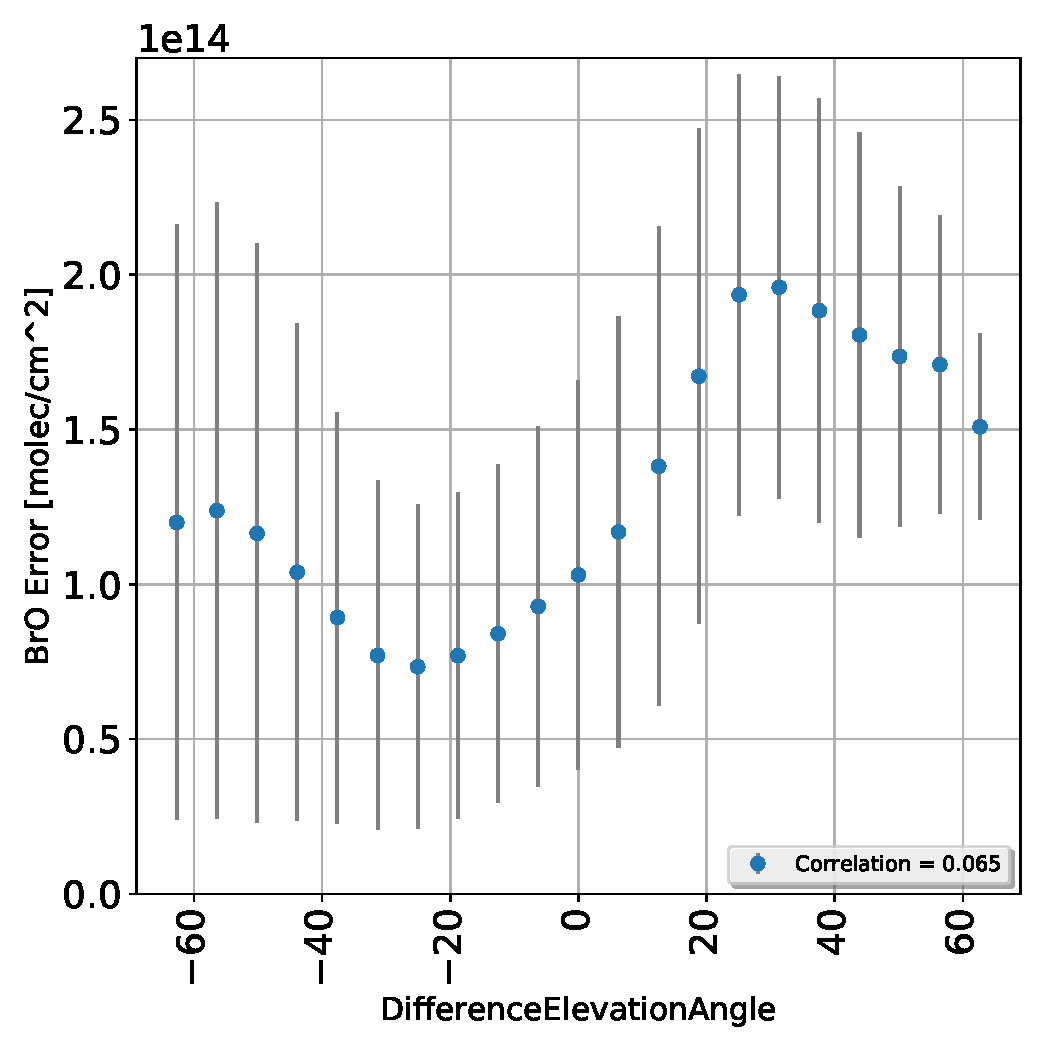
\includegraphics[width=0.3\linewidth]{Bilder/DEpendencoOfBrOErrorOnVariables_absolutedep/D2J2200_0BrOERR_DiffElevAngle_Nevad}}
		\subfigure[]{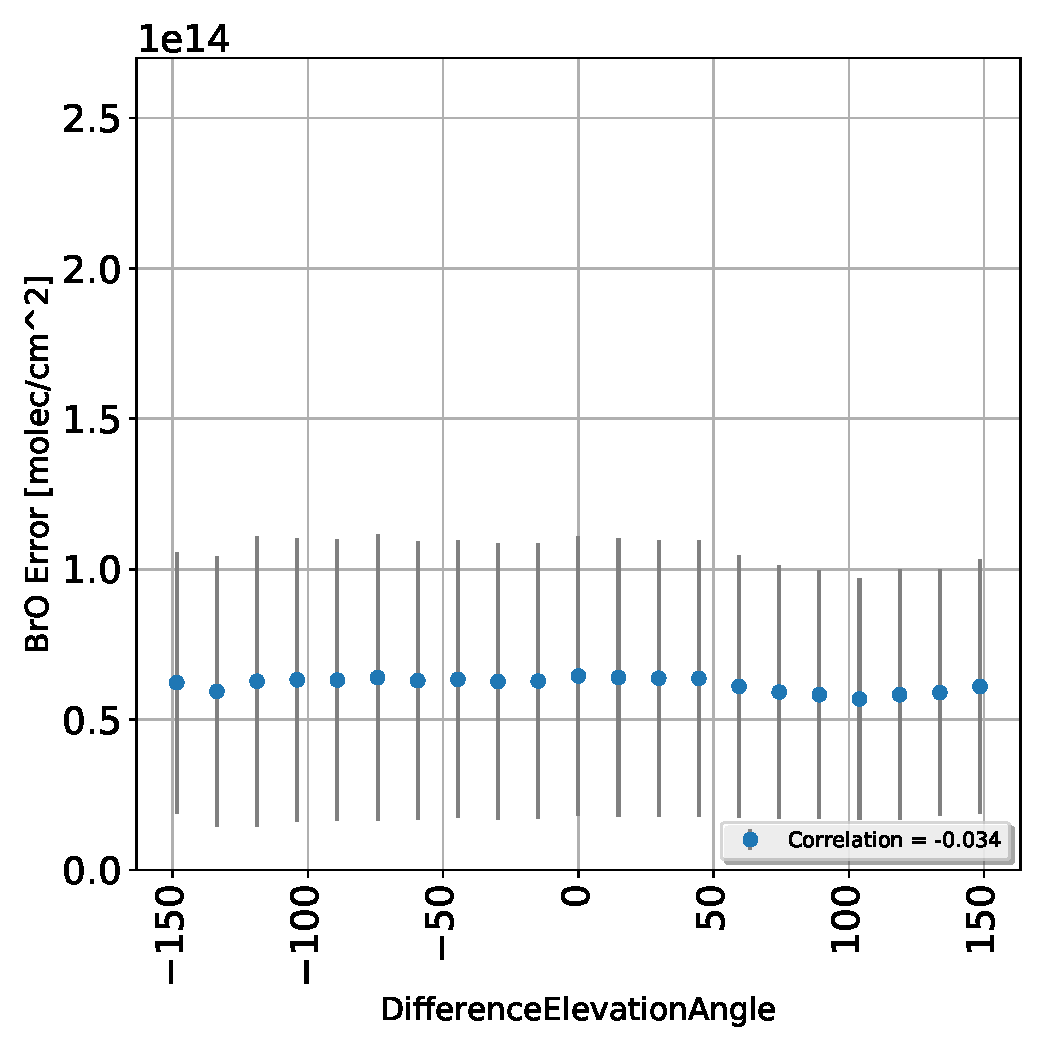
\includegraphics[width=0.3\linewidth]{Bilder/DEpendencoOfBrOErrorOnVariables_absolutedep/D2J2201_0BrOERR_DiffElevAngle_Nevad}}
		\caption{The BrO Measurement Error as a function of the Elevation Angle. To evaluate the plume spectra all reference spectra with a temporal distance of no longer than two weeks are used. We can't see any significant correlation.}
		\label{fig:diffeleangle}
	\end{figure}
	The elevation angle describes the angle between the horizon and the zenith. When using the plume spectrum and the reference spectrum of the same time, the difference in elevation angle cannot be zero, since the location of the plume does not coincidence with the location of the reference.\\
	The \ce{BrO} error doesn't depend significantly on the difference between the Elevation Angles. This could have several reasons. One problem is, that the Elevation Angle of Plume and Reference spectrum is not the same. This could also be a reason of uncertainty of the evaluations of the plume spectrum.

	\begin{itemize}
		\item The BrO error as a function of the difference in colour index is also symmetric around zero for all instruments, except  D2J2200\_0 at Nevado Del Ruiz. 
		\item Only D2J2140\_0 shows a minimum of the BrO error at a difference in Elevation Angle of 0$^{\circ}$. The BrO error curve from D2J2200\_0 shows a minimum at around -20$^{\circ}$.
		\item Because there is no significant dependence between BrO error and the difference in Elevation Angle it will not be considered in further analysis.
	\end{itemize}
	\begin{table}[h]
		\begin{tabular}{|p{2cm}|p{2cm}|p{2cm}|p{2cm}|p{2cm}|p{2cm}|}
			%	\toprule
			Instrument	&D2J2140\_0&I2J8546\_0& I2J8548\_0&D2J2200\_0&D2J2201\_0\\
			\toprule
			Slope& 1.73e+8& 1.55e+10  &-9.00e+9 &2.92e+11&-3.96e+10\\
			\midrule
			Correlation&
			0.000&
			-0.010&
			0.012&
			0.065&
			-0.034\\
			\midrule
			Zero point&4.77e+13&4.23e+13&3.78e+13&8.37e+13 &6.44e+13 \\
			\bottomrule
		\end{tabular}
	\end{table}

	\subsection{Exposure Time}
	\begin{figure}
		\subfigure[]{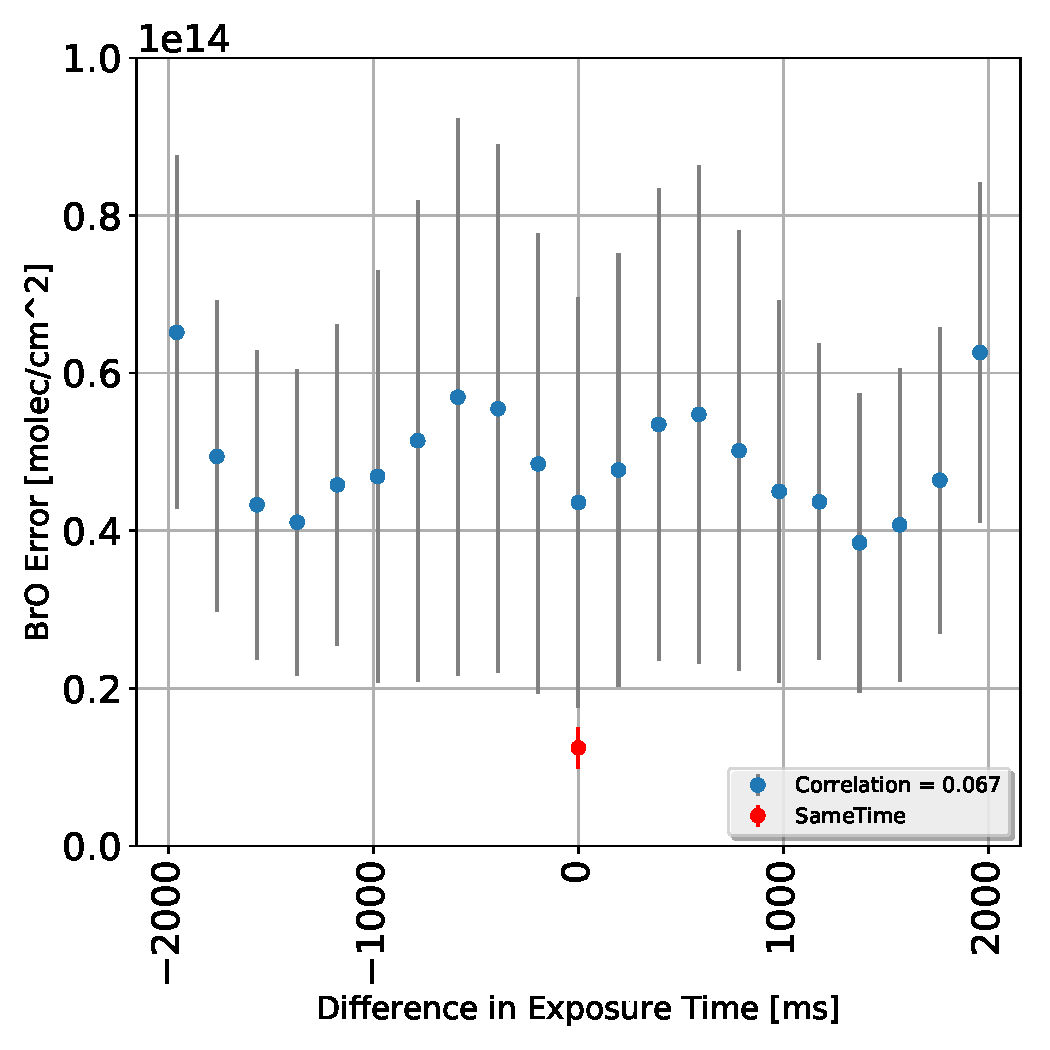
\includegraphics[width=0.3\linewidth]{Bilder/DEpendencoOfBrOErrorOnVariables_absolutedep/D2J2140_0BrOERR_DiffExpTime_Tungu}}
		\subfigure[]{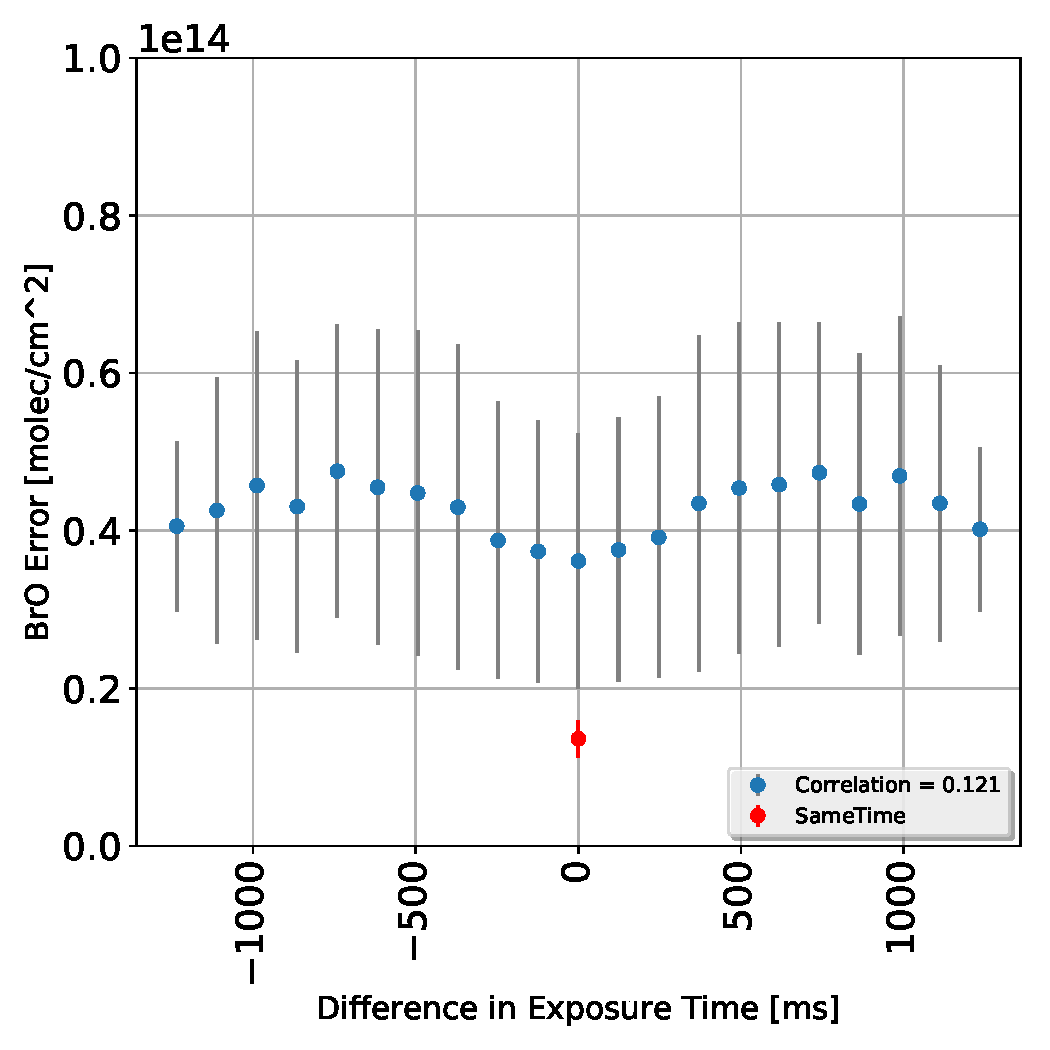
\includegraphics[width=0.3\linewidth]{Bilder/DEpendencoOfBrOErrorOnVariables_absolutedep/I2J8546_0BrOERR_DiffExpTime_Tungu}}
		\subfigure[]{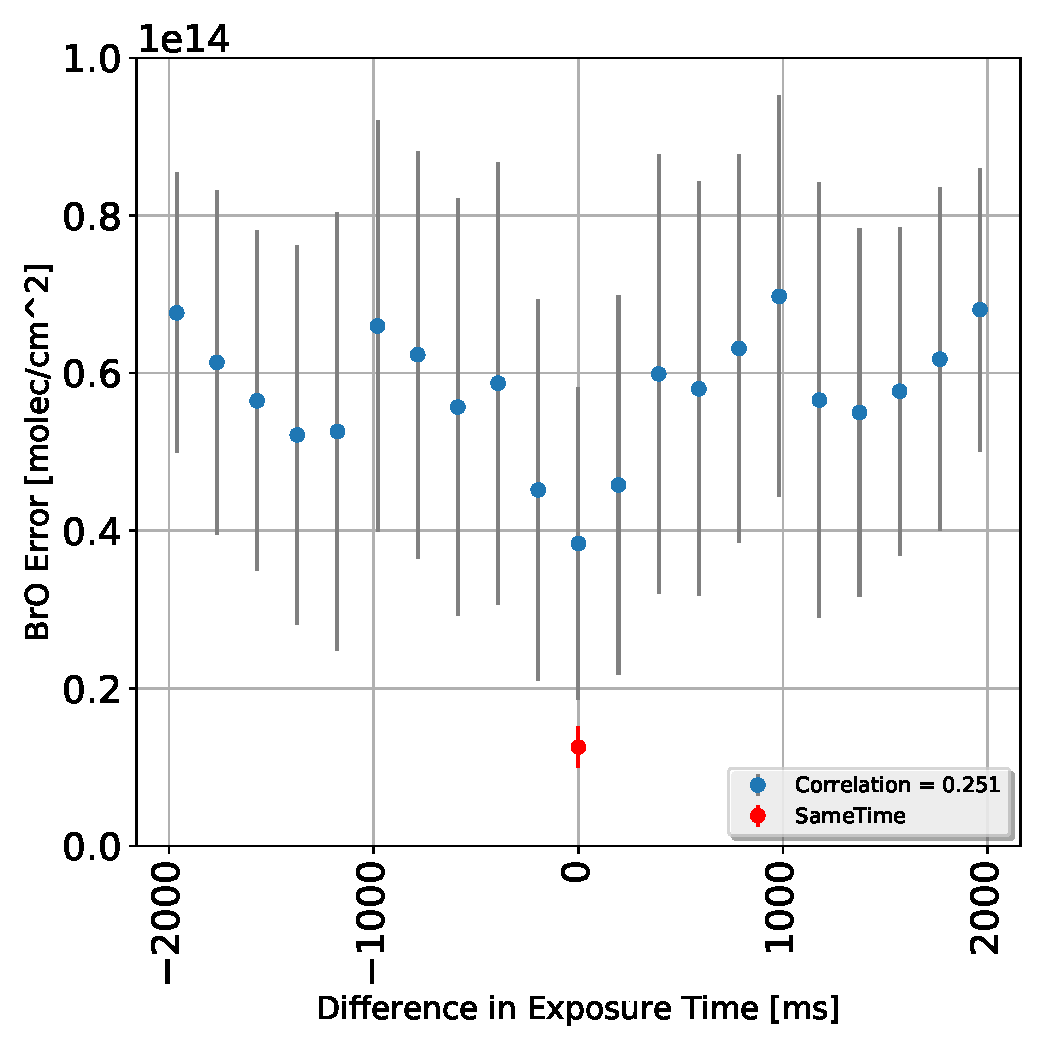
\includegraphics[width=0.3\linewidth]{Bilder/DEpendencoOfBrOErrorOnVariables_absolutedep/I2J8548_0BrOERR_DiffExpTime_Tungu}}
		\centering
		\subfigure[]{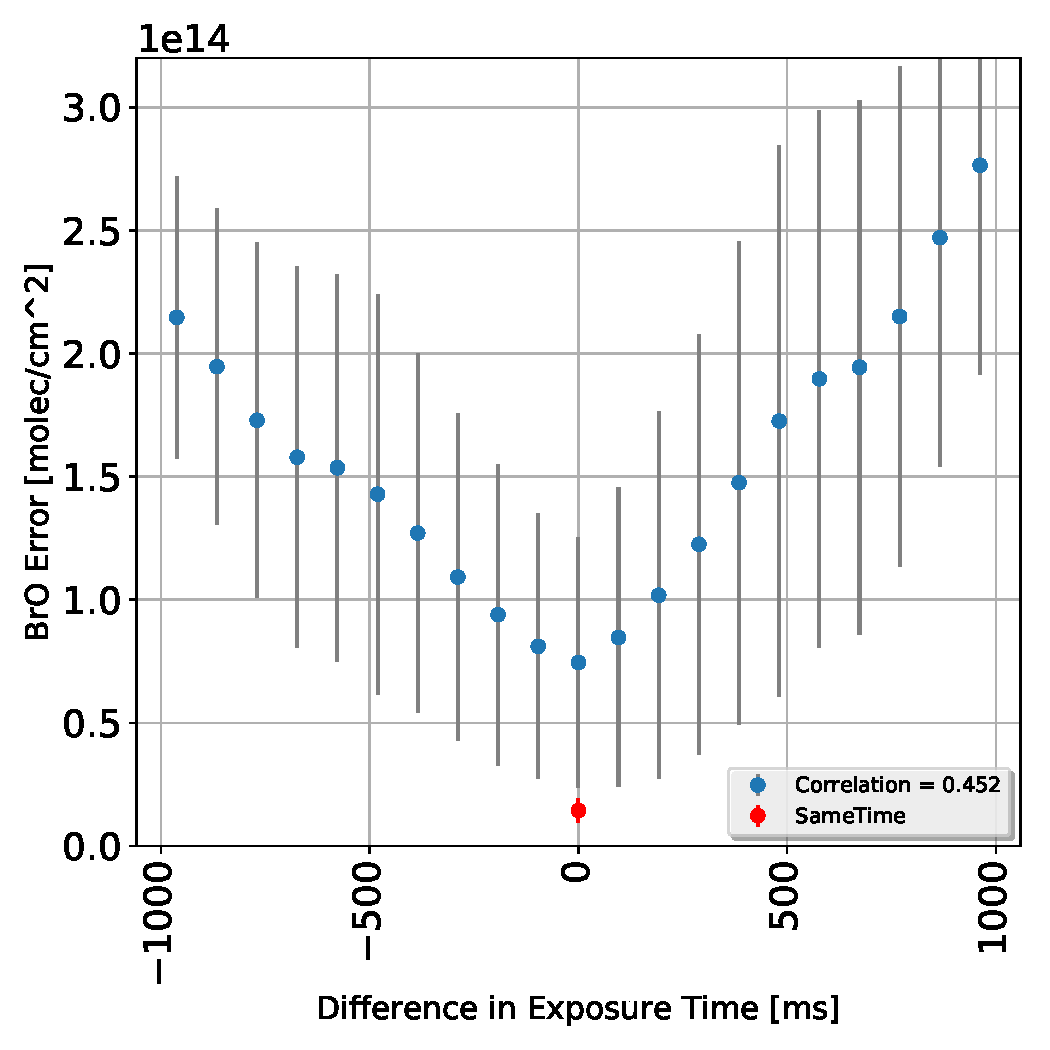
\includegraphics[width=0.3\linewidth]{Bilder/DEpendencoOfBrOErrorOnVariables_absolutedep/D2J2200_0BrOERR_DiffExpTime_Nevad}}
		\subfigure[]{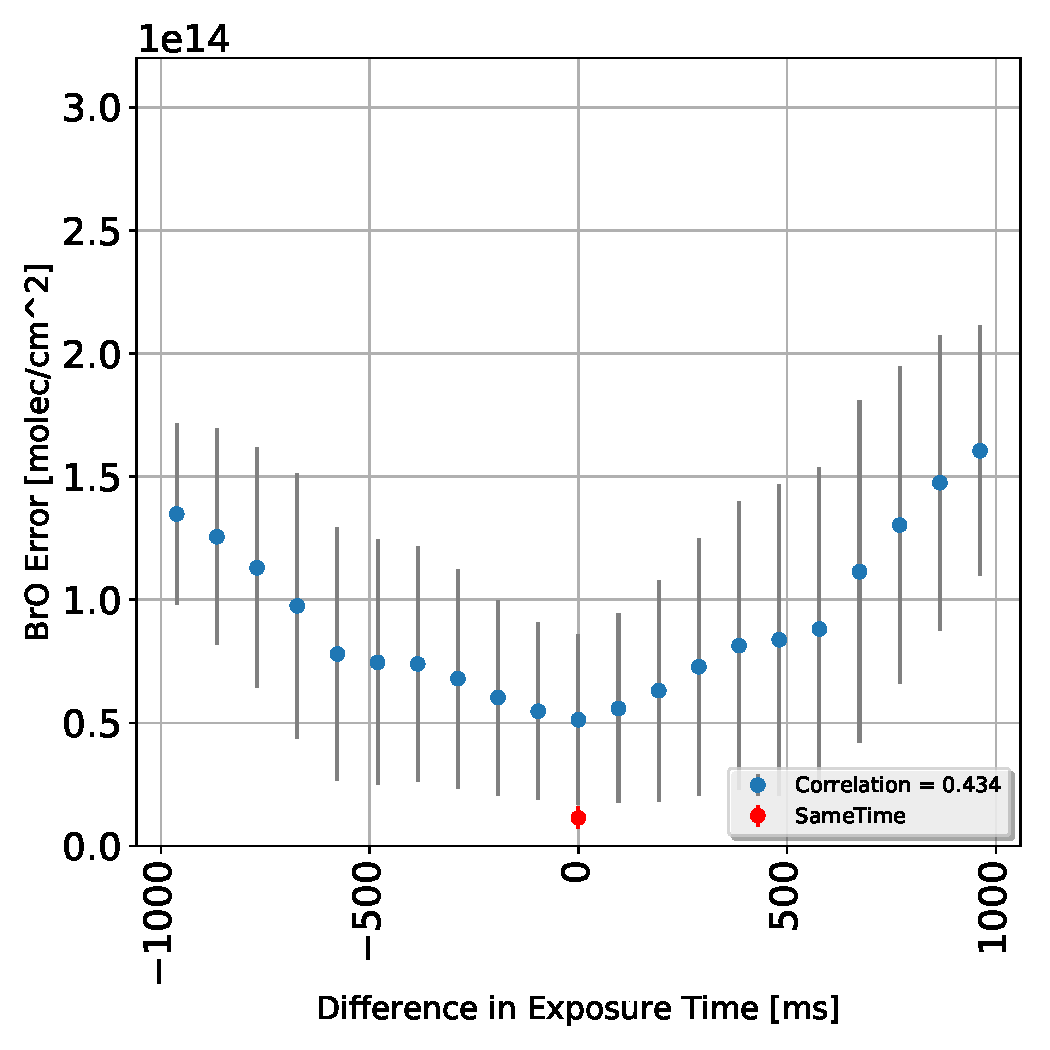
\includegraphics[width=0.3\linewidth]{Bilder/DEpendencoOfBrOErrorOnVariables_absolutedep/D2J2201_0BrOERR_DiffExpTime_Nevad}}
		\caption{The BrO Measurement Error as a function of the difference of exposure time between measuring the reference and the plume are shown. To evaluate the plume spectra all reference spectra with a temporal distance of no longer than two weeks are used. A increase of the BrO Error with the distance in exposure time is observably.}
		\label{fig:diffexptime}
	\end{figure}
	The Exposure Time is a degree of sky lightness.The  exposure time is the length of time the sensor of the NOVAC instrument is exposed to light. In one scan the exposure time is set constant. The amount of light that reaches the film or image sensor is proportional to the exposure time. The exposure time is adjusted in the way that the maximum intensity does not overly the capacity of the sensor.\\
	We can observe an small dependency of the \ce{BrO} error on the Exposure time at Tungurahua and Nevado Del Ruiz as it is shown in \cref{fig:diffexptime}
	\begin{itemize}
		\item The BrO error as a function of the difference in Exposure Time is also symmetric around zero for all observed instruments, thus the absolute difference in the Exposure Time is sufficient for the evaluating.
		\item The instruments at Tungurahua does not show significantly dependence on the Exposure Time, even though there is always a minimum of the BrO Error at a difference of the Exposure Time of 0ms.
		\item Nevado Del Ruiz shows a stronger correlation between the BrO error and the Exposure Time.
	\end{itemize}
	\begin{table}[h]
		\begin{tabular}{|p{2cm}|p{2cm}|p{2cm}|p{2cm}|p{2cm}|p{2cm}|}
			%	\toprule
			Instrument	&D2J2140\_0&I2J8546\_0& I2J8548\_0&D2J2200\_0&D2J2201\_0\\
			\toprule
			Slope& 5.54e+9&1.54e+10 &3.04e+10&1.72e+11&9.37e+10\\
			\midrule
			Correlation&0.067
			&0.121&
			0.251&
			0.452&
			0.434\\
			\midrule
			Zero point&4.63e+13&3.58e+13& 3.87e+13& 6.88e+13& 4.68e+13\\
			\bottomrule
		\end{tabular}
	\end{table}

	\begin{itemize}
		\item The \ce{BrO} Error increases with the exposure time differences as\\
		\begin{align*}
		\rightarrow&  BrO_{Error} = f(ext. P)+ 1.92\cdot10^{12}\cdot\frac{\Delta ET}{10^{-2}s} + \mathcal{O}\left(\right) & Tungurahua\\
		\rightarrow&  BrO_{Error} = f(ext. P)+ 1.0\cdot10^{13}\cdot\frac{\Delta T}{10^{-2}s} + \mathcal{O}\left(\right) & Nevado Del Ruiz\\
		\end{align*}
	\end{itemize}
	\subsection*{Dependency of external parameters on each other}
	In all those discussions on the impact of the external parameter on the retrieved BrO error the  dependency of the external parameter on each other where neglected. It is plausible that the temperature correlates with the cloudiness or the lightness due to sunlight. Therefore the correlation of the Exposure Time with the BrO error could be a result of the correlation of the Temperature with the BrO error. \cref{fig:difference-in-exposure-time-msdifference-in-temperature-ctungu} shows an example of the dependency of external parameters on each other. The Difference in Temperature as a function of the Difference in Exposure Time. The BrO error is color-coded. \\
	All correlations between the external parameters are shown in \cref{fig:varcorrelationmatrix}. \Cref{fig:varcorrelationmatrix} show discrete correlation values from 0.3 to 1. Correlations below 0.3 are ignored. Small plus and minus signs indicate whether the correlation is negative ore positive. 
	The difference in temperature correlates with the difference in daytime (Correlation of $\approx$ 0.5) with the difference in Exposure Time (Correlation of $\approx$ 0.4). The difference in temperature also slightly correlates with the difference in Colorindex (Correlation of $\approx$ 0.3) and the temporal difference (Correlation of $\approx$ 0.3) probably due to long term changes in Temperature. Furthermore the difference in Exposure Time correlates with the daytime and the colorindex (Correlation of $\approx$ 0.4).\\
	\begin{figure}
		\centering
		\includegraphics[width=0.7\linewidth]{"../Ausarbeitung/Uebersicht/Bilder/Difference in Exposure Time [ms]_Difference in Temperature [C]_Tungu"}
		\caption{A example of the dependency of external parameters on each other. The difference in Temperature as a function of the Exposure Time. Data from Tungurahua}
		\label{fig:difference-in-exposure-time-msdifference-in-temperature-ctungu}
	\end{figure}
	\begin{figure}
		\centering
		\includegraphics[width=1\linewidth]{Bilder/varCorrelation_matrix}
		\caption{Correlation matrix of the external parameters. The correlation is discrete colour coded. Positive correlation is labeled with a plus whereas negative correlation is labeled with a minus.}
		\label{fig:varcorrelationmatrix}
	\end{figure}
%
		\textbf{Difference of Temperature on  Difference of Exposure Time}
		\begin{equation}
		\Delta T =  -26.32\cdot \Delta ExpTime + 2\cdot 10^{-15}
		\end{equation}
		
		\textbf{Difference of Temperature on  Difference of colorindex}
		\begin{equation}
		\Delta T = 0.0022\cdot \Delta ColIdX +2\cdot 10^{-19}
		\end{equation}
		
				\textbf{Difference of Temperature on  Difference of Day time}
		\begin{equation}
		\Delta T =0.262\cdot \Delta daytime -4\cdot 10^{-17}
		\end{equation}
		
						\textbf{Difference of Temperature on  Difference of Elevation angle}
		\begin{equation}
		\Delta T =1.08\cdot \Delta Elev Angle -1\cdot 10^{-16}
		\end{equation}

		\textbf{Difference of Exposure on  Difference of  Col Idx}
		\begin{equation}
		\Delta Exposure  =-6.22\cdot 10^{-5} \Delta Col Idx  +1\cdot 10^{-18}
		\end{equation}
		
				\textbf{Difference of  Exposure on  Difference of Day time}
		\begin{equation}
		\Delta Exposure  =-0.004\cdot \Delta daytime -1\cdot 10^{-17}
		\end{equation}
		
						\textbf{Difference of  Exposure  on  Difference ofElevation angle}
		\begin{equation}
		\Delta Exposure  =-0.047\cdot \Delta  ElevAngle +3\cdot 10^{-16}
		\end{equation}


		\textbf{Difference of  Colorindex  on  Difference of Day time}
		\begin{equation}
		\Delta ColIdX  =4.51\cdot \Delta daytime-1.2\cdot 10^{-15}
		\end{equation}
		
		\textbf{Difference of  Colorindex  on  Difference of Elevation angle}
		\begin{equation}
		\Delta ColIdX  =-52\cdot \Delta ElevAngle+ 1.45\cdot 10^{-14}
		\end{equation}
		
				\textbf{Difference of  Colorindex  on  Difference of Elevation angle}
		\begin{equation}
		\Delta ColIdX  =3.5\cdot \Delta ElevAngle-6\cdot 10^{-16}
		\end{equation}
	To eliminate the correlation between the external parameters the BrO error dependency on one external parameter where calculated by keeping the differences in the other external parameters constant. The results can be seen in \cref{fig:DiffExpTime} ( Tungurahua) and \cref{fig:DiffExpTimeNevad} (Nevado Del Ruiz). When comparing the correlations of the data from \cref{fig:DiffExpTime} and \cref{fig:DiffExpTimeNevad}  to the correlations of 
	\cref{fig:difftemp} to \cref{fig:diffexptime} a large reduction of the correlation is obvious. Only the difference in Temperature still shows a significant correlation to the BrO error. However the minimal BrO error coincidence in almost all cases with a difference in external parameters of zero. And the variability (visualized as the length of the grey bars) increases with increasing difference in external parameters for almost all cases.\\
	\\
	Besser erklähren, auch, dass die Auswertung am Enden besser läuft wenn man sie auch mitreinzählen lasst\\
	\\
	\begin{figure}
			\subfigure{\includegraphics[width=0.3\linewidth]{Bilder/BrOError_onVariables_050218/I2J8546_0DiffTemp_Tungu}}
			\subfigure{\includegraphics[width=0.3\linewidth]{Bilder/BrOError_onVariables_050218/I2J8548_0DiffTemp_Tungu}}
			\subfigure{\includegraphics[width=0.3\linewidth]{Bilder/BrOError_onVariables_050218/D2J2140_0DiffTemp_Tungu}}
		\subfigure{\includegraphics[width=0.3\linewidth]{Bilder/BrOError_onVariables_050218/I2J8546_0DiffColidx_Tungu}}
		\subfigure{\includegraphics[width=0.3\linewidth]{Bilder/BrOError_onVariables_050218/I2J8548_0DiffColidx_Tungu}}
		\subfigure{\includegraphics[width=0.3\linewidth]{Bilder/BrOError_onVariables_050218/D2J2140_0DiffColidx_Tungu}}

		\subfigure{\includegraphics[width=0.3\linewidth]{Bilder/BrOError_onVariables_050218/I2J8546_0DiffDaytime_Tungu}}
		\subfigure{\includegraphics[width=0.3\linewidth]{Bilder/BrOError_onVariables_050218/I2J8548_0DiffDaytime_Tungu}}
		\subfigure{\includegraphics[width=0.3\linewidth]{Bilder/BrOError_onVariables_050218/D2J2140_0DiffDaytime_Tungu}}

		\subfigure[I2J8546\_0]{\includegraphics[width=0.3\linewidth]{Bilder/BrOError_onVariables_050218/I2J8546_0DiffExpTime_Tungu}}
		\subfigure[I2J8548\_0]{\includegraphics[width=0.3\linewidth]{Bilder/BrOError_onVariables_050218/I2J8548_0DiffExpTime_Tungu}}
		\subfigure[D2J2140\_0]{\includegraphics[width=0.3\linewidth]{Bilder/BrOError_onVariables_050218/D2J2140_0DiffExpTime_Tungu}}
		\caption{DiffExpTime at Tungurahua}
		\label{fig:DiffExpTime}
	\end{figure}


		\begin{figure}
			\centering
			\caption{BrO Error as a function of the external while measering the Plume and the Reference at Nevado del ruiz}
			\subfigure{\includegraphics[width=0.3\linewidth]{Bilder/BrOError_onVariables_050218/D2J2201_0DiffTemp_Nevad}}
			\subfigure{\includegraphics[width=0.3\linewidth]{Bilder/BrOError_onVariables_050218/D2J2200_0_DiffTemp_Nevad}}\\

			\centering
			\subfigure{\includegraphics[width=0.3\linewidth]{Bilder/BrOError_onVariables_050218/D2J2201_0DiffColidx_Nevad.pdf}}
			\subfigure{\includegraphics[width=0.3\linewidth]{Bilder/BrOError_onVariables_050218/D2J2200_0_DiffColidx_Nevad.pdf}}

			\subfigure{\includegraphics[width=0.3\linewidth]{Bilder/BrOError_onVariables_050218/D2J2201_0DiffDaytime_Nevad}}
			\subfigure{\includegraphics[width=0.3\linewidth]{Bilder/BrOError_onVariables_050218/D2J2200_0_DiffDaytime_Nevad}}


			\subfigure[D2J2201\_0]{\includegraphics[width=0.3\linewidth]{Bilder/BrOError_onVariables_050218/D2J2201_0DiffExpTime_Nevad}}
			\subfigure[D2J2200\_0]{\includegraphics[width=0.3\linewidth]{Bilder/BrOError_onVariables_050218/D2J2200_0_DiffExpTime_Nevad}}
			\label{fig:DiffExpTimeNevad}
		\end{figure}
	
	\section{BrO dependence on external parameters}
	hier kommt ganz viel text hin
	\begin{figure}
		\subfigure[]{
		\includegraphics[width=0.5\linewidth]{"Bilder/OnePlumeMoreRefs_plumedate_081203_1646/D2J2140_0_6_02_18_DiffTemperature [C]_BrO"}}
		\subfigure[]{\includegraphics[width=0.5\linewidth]{"Bilder/OnePlumeMoreRefs_plumedate_081203_1646/D2J2140_0_plumeat12Temperature [C]_BrO_TemporalDiff"}}	
		\caption{}
		\label{fig:d2j2140060218difftemperature-cbro}		
	\end{figure}

	
	%--------------------------------------------------------------------------------------------------------------
	\chapter{Method}
	Based on the findings about the influence of external parameters on the \ce{BrO} error we developed an algorithm which is able to pick an appropriate volcanic-trace-gas free reference.\\ 
	The first step is, to evaluate every reference with solar atlas spectrum, to check for contamination.	A Spectrum is treated as contaminated if the \ce{SO2} column density of the reference (evaluated with a solar atlas spectrum) is larger as 2$\cdot 10^{17}\frac{molec}{cm^2}$.\\
	\\
	If the reference is contaminated:
	\begin{figure}
\centering
\includegraphics[width=0.7\linewidth]{Bilder/Cont}
\caption{}
\label{fig:Cont}
\end{figure}

	\begin{itemize}
		\item We have a list of possible references where all references are not contaminated and the temporal distance to the plume date is no longer than 14 days.
		\item we calculate of all possible references the differences in the external parameters
		\item We use the analysis of external parameters described above to estimate the \ce{BrO} error of all references
		\item We choose the reference with the smallest estimated \ce{BrO} error as new reference
		\item We evaluate the plume spectra with the new reference.
	\end{itemize}

	%
	The assumption is, that the \ce{BrO} error $\epsilon_{BrO}$ can be described as the sum of $\epsilon_{0}$ and the deviation of $\epsilon_{BrO}$ with respect to all external parameters. $\epsilon_{0}$ is the \ce{BrO} error when evalute the plume spectrum with the "same-time-reference", it is determined due to the accurateness of the NOVAC-instruments.
	\begin{align}
		\epsilon_{BrO} &=  \epsilon_{0}+\frac{d\epsilon}{dt}+\frac{d\epsilon}{d ^{\circ}}+\frac{d\epsilon}{dT}+\frac{d\epsilon}{ddt} +\frac{d\epsilon}{dc} + \mathcal{O}\left(OE\right) \\
		\rightarrow \Delta \epsilon_{BrO} &= \epsilon_{BrO} - \epsilon_{0} =\frac{d\epsilon}{dt}+\underbrace{\frac{d\epsilon}{d ^{\circ}}}_{=0}+\frac{d\epsilon}{dT}+\frac{d\epsilon}{ddt} +\frac{d\epsilon}{dc} + \mathcal{O}\left(OP\right) 
		\label{calc:err}
	\end{align}
	With $\epsilon_{BrO}$ describes the \ce{BrO} Error, t: time between plumetime and referencetime, T, temperaure; dt: daytime, c: colorindex, OP: other excluded external parameters\\
	The task occurring at this stage is to find the best representation for the deviations. An then find the reference which minimize $\Delta \epsilon_{BrO} $\\
	%
	\\
	%
	The easiest way is to just calculate the \ce{BrO} error of all possible references for every plume. Using this method we would be able to just choose the reference where the \ce{BrO} error is minimal. But this takes to much time since the evaluation would be proportional to the number of possible references because the evaluation need to be done for every plume-reference pair. Doing the evaluation for every plume-reference pair would make it impossible to do the evaluation in real, or near real time.\\
	%
	But we use this optimal evaluation to rate our model and compare them among each other. The optimal evaluation always choose the reference with the smallest absolute error. We don't use the relative error due to his vulnerability. Using the relative error could lead to a less preciseness.\\
	%
	\\
	Hier ein Bild, das eine Plume gegen viele referencen auswertet und hier die Abweichungen zeigt\\
	\\
	%
	The results of the algorithm which chooses the reference automatically are described relative to an optimal evaluation. If the relative error is larger than 5 we don't use the data.\\
	\\
	We tried several methods for choosing the best reference based on the analysis of external parameters. Fitting the data with a first order polynomial brought the best results.
	
	
	\section{Fit data}
	The following chapter analyses the possibility of fitting the data by a first order polynom. \Cref{fig:difftemp}-\Cref{fig:diffexptime} show the BrO error as a function of external parameters. Hereby are the curves symetric around zero differences in the respective external parameter. Therefore it is not necessary to distinguish between positive or negative deviations from the equal surrounding conditions. Thus the absolute differences can be taken.\\
	\\
	%
	A linear approximation of the BrO error as function of the considered external parameter leads to a variation of  \cref{calc:err} :
	With linear differentiations of the BrO error with respect to the respective external parameters \cref{calc:err} can be written as:	
	\begin{equation}
		\Delta \epsilon_{BrO} = a_{t}\cdot\Delta t+a_{ET}\cdot\Delta ET+a_{T}\cdot\Delta T+a_{dt}\cdot\Delta dt +a_{c}\cdot\Delta c + \mathcal{O}\left(OP\right)
		\label{calc:delterr}
	\end{equation}
	%
	To determine the coefficients $a_{x}$ (\cref{calc:delterr}) the data as from \cref{fig:difftemp}-\ref{fig:diffexptime} where used.  The fitting was done with an ordinary least square linear regression. In particular we used the python function Linear Regression from the library sklearn \cite{SKlearn}. \\
	
	As can be seen in \Cref{Chap:BROErr} the impact of the different external parameters change for every instrument depending on the location and the instrument themself. 
	Whereas the BrO error not show any dependence on some external parameter at some instrument the Error has very strong dependence on the same external parameter at another instrument. An example is the correlation between BrO error of 0.6 at D2J2201\_0 (Nevado Del Ruiz) and a correlation of 0.16 at I2J8546\_0 at the Tungurahua volcano.
	To get a more stable algorithm less external parameter are preferable. Thus we need to distinguish between the stability of the fit, which favours less external parameters and quality of the fit, which favours more external parameters. 
	A preferable solution is, to find a solution which is valid for all instruments at the same time to save calculation time. 
	One possibility is to use all external parameter where the correlation is above a certain number, since we want to get a selection valid for all instruments there are two possibilities: The first one is we decide by using the mean correlation of all instruments, the second option is to use the highest correlation
	
	\begin{table}[h]
		\begin{tabular}{|p{4cm}|p{3cm}|p{3cm}|}
			&  Mean -Correlation&  Highest   -Correlation\\
			\toprule
			Temporal Difference&0.798&	0.92\\
			\midrule
			Temperature &0.798&	0.92\\
			\midrule
			Colorindex &0.3108&	0.409\\
			\midrule
			Exposure Time &0.265&	0.452\\
			\midrule
			Elevation Angle &0.02&	0.067\\
			\midrule
			Daytime &0.395&	0.631\\
			\bottomrule
		\end{tabular}
	\end{table}
	\begin{figure}
		\subfigure[Nevado Del Ruiz]{
			\includegraphics[width=0.5\linewidth]{"Bilder/WelcheEP/Nevado Del Ruiz"}}
		\subfigure[Tungurahua]{
			\includegraphics[width=0.5\linewidth]{Bilder/WelcheEP/Tungurahua}}
		\caption{}
		\label{fig:WelcheEP}
	\end{figure}
	To answer this question quantitatively for the fitting routine we evaluated data of Tungurahua and Nevado Del Ruiz with different combinations of the external parameter described in \cref{Chap:BROErr}. Since we could not observe any correlation between the BrO Error and the Elevation angle the external parameter elvation angle was neglected in this analysis. To rate the results for the single instruments (three at Tungurahua and two at Nevado Del Ruiz) the difference to the "optimal evaluation" (explained in \ref{optimal evaition}) was used. Hereby the factor x, a quantity which describes the distinction between the optimal-Method and the contamination based method serves as indicator:
	\begin{equation}
	X = \frac{1}{n}\sum_{k}^{n} \frac{EContBased_{ k}}{EOpt_{ k}}
	\label{eq:mean}
	\end{equation}
	$n$ is the total amount of contaminated spectra, $EOpt$ is the BrO error, in the optimal-evaluation, $EContBased$ is the BrO error, in the contamination based-evaluation. 
	\Cref{fig:WelcheEP} shows the calculations of the x factor for th e Tungurahua and the Nevado Del Ruiz volcano. The x-axis shows the external parameter used for the factor X. The y-axis shows the added factors x for every instrument at the volcanoes. The x factors were weighted with the percentage amount of data.
	The factors X change from instrument to instrument. The results for every instrument can be seen in the appendix (\cref{fig:I2J8548}). The factors X range from 1.18 to 1.42. Thus the difference is not that large. 
	If using the median and not the mean as described in \cref{eq:mean} our method is even better than the "optimal method". (soll das beschrieben werden wenn ja hier)\\
	As in \Cref{fig:WelcheEP} can be seen  for both volcanoes the x factor is minimal for the combination of the following external parameters:\\
	
	\begin{table}[h!]
			\begin{tabular}{cccc}
		$\bullet$ Temperature & $\bullet$ Daytime&  $\bullet$ Exposure Time & $\bullet$ Temporal Difference\\
		\label{tab:importantexternalParam}
		\end{tabular}
	\end{table}
%	

	For the final algorithm this combination of external parameters is used.
	The coefficients $a_{x}$ were calculated for each instrument at Nevado Del Ruiz and Tungurahua. Furthermore the coefficients $a_{x}$ are calculated with the combined data from all instruments installed at one volcano. The results for the Nevado Del Ruiz volcano can be found in \cref{tab:coefNevad} and for the Tungurahua volcano in \cref{tab:coefTung}.
	\begin{table}
		\subfigure{
			\begin{tabular}{c|c|c}
				\toprule
				Constant\\
				\toprule
				$a_{T}$\\
				\midrule
				$a_{ET}$\\
				\midrule
				$a_{t}$\\
				\midrule
				$a_{dt}$\\
				\midrule
				$a_{c}$\\
				\bottomrule
		\end{tabular}}
		\subfigure[Data of Nevado Del Riz D2J2201\_0]{
			\begin{tabular}{c|c}
				\toprule
				value & import\\
				\toprule
				 7.34e+12&0.840\\
				\midrule
				1.55e+10&0.045\\
				\midrule
				-2.6e+09& 0.0\\
				\midrule
				1.81e+12&0.091\\
				\midrule
				2.30e+13& 0.031\\
				\bottomrule
		\end{tabular}}
	\subfigure[Data of Nevado Del Riz D2J2200\_0]{
		\begin{tabular}{c|c|c}
			\toprule
			value & import \\
			\toprule
		 	1.16e+13&0.908 \\
			\midrule
			2.81e+10& 0.046\\
			\midrule
			-1.7e+09& 0.0\\
			\midrule
			1.08e+12&0.034\\
			\midrule
			3.59e+13& 0.016\\
			\bottomrule
	\end{tabular}}
	\subfigure[Data of Nevado Del Both Instruments]{
		\begin{tabular}{c|c|c}
			\toprule
			value & import \\
			\toprule
			1.07e+13&0.973 \\
			\midrule
			3.48e+10&  0.070\\
			\midrule
			-9.1e+08& 0.0\\
			\midrule
			 1.52e+11&0.006\\
			\midrule
			 -6.81e+13& -0.047\\
			\bottomrule
	\end{tabular}}
	\caption{(a)Data from Nevado Del Ruiz from the D2J2201\_0 instrument. All external parameter where taken into account. $\epsilon_{0} = =  5.404e+12$
			(b)Data from Nevado Del Ruiz from the D2J2200\_0 instrument. All external parameter where taken into account. $\epsilon_{0} = =  1.105e+13$ (c) Data from Nevado Del Ruiz from both instrument. All external parameter where taken into account. $\epsilon_{0} = 1.260e+13$}
		\label{tab:coefNevad}
	\end{table}	
	\begin{table}
	\subfigure{
		\begin{tabular}{c|c|c}
			\toprule
			Constant\\
			\toprule
			$a_{T}$\\
			\midrule
			$a_{ET}$\\
			\midrule
			$a_{t}$\\
			\midrule
			$a_{dt}$\\
			\midrule
			$a_{c}$\\
			\bottomrule
	\end{tabular}}
	\subfigure[Data of Tungurahua D2J2201\_0]{
		\begin{tabular}{c|c}
			\toprule
			value & import\\
	\end{tabular}}
	\subfigure[Data of Tungurahua D2J2200\_0]{
		\begin{tabular}{c|c|c}
			\toprule
				value & import \\

	\end{tabular}}
	\subfigure[Data of Tungurahua Both Instruments]{
		\begin{tabular}{c|c|c}
			\toprule
			value & import \\
		
	\end{tabular}}
		\caption{(a)Data from Tungurahua  from the instrument. All external parameter where taken into account. $\epsilon_{0} = =  5.404e+12$
			(b)Data from Tungurahua from the  instrument. All external parameter where taken into account. $\epsilon_{0} = =  1.105e+13$ (c) Data from Tungurahua from all instrument. All external parameter where taken into account. $\epsilon_{0} = 1.260e+13$}
		\label{tab:coefTung}
	\end{table}			
	\begin{figure}
		\centering
		\includegraphics[width=0.7\linewidth]{E:/Masterarbeit/Analyse_minSO2/percentage_minSO2}
		\caption{}
		\label{fig:percentageminso2}
	\end{figure}
	\begin{figure}
		\centering
		\includegraphics[width=0.7\linewidth]{E:/Masterarbeit/Analyse_minSO2/data_minSO2}
		\caption{}
		\label{fig:dataminso2}
	\end{figure}
	Analyse ob der spass mit den correlations zusammenhaengt
	\section{Other approaches}

	$\bullet$ In the optimal results are 15$\%$ valid data
	\begin{itemize}
		\item We also tried other possibilities than fitting to find the reference where the \ce{BrO} error is minimal. In the following we present two additional possibilities but compared to fitting the results are not as good.
	\end{itemize}
	\subsection{Nearest neighbours}
	\begin{itemize}
		\item Description of the Nearest Neighbours Method
	\end{itemize}
		\textcolor{red}{Nearest neighbor search (NNS), as a form of proximity search, is the optimization problem of finding the point in a given set that is closest (or most similar) to a given point. Closeness is typically expressed in terms of a dissimilarity function: the less similar the objects, the larger the function values. Formally, the nearest-neighbor (NN) search problem is defined as follows: given a set S of points in a space M and a query point q$\in$ M, find the closest point in S to q. Donald Knuth in vol. 3 of The Art of Computer Programming (1973) called it the post-office problem, referring to an application of assigning to a residence the nearest post office. A direct generalization of this problem is a k-NN search, where we need to find the k closest points.	
		Most commonly M is a metric space and dissimilarity is expressed as a distance metric, which is symmetric and satisfies the triangle inequality. Even more common, M is taken to be the d-dimensional vector space where dissimilarity is measured using the Euclidean distance, Manhattan distance or other distance metric. However, the dissimilarity function can be arbitrary. One example are asymmetric Bregman divergences, for which the triangle inequality does not hold.}
	\subsection{Iterative}
	\begin{itemize}
		\item Description of the iterative Method
	\end{itemize}
	The idea of the iterative method was, that the importance of the individual external parameters are very different, that means if we have the list of possible references, we took all referenes where the temperature difference is minimal, so we get a new, much smaller list of possible referenecs. From this list we choose all references where the next external parameter for example the daytime is minimal and get again a new list. We proceed this way with the following external parameters. We experiment with the sequence of the parameters, to increase the success of the method. The final sequence was:
	\begin{equation*}
	Temperature \bullet ................
	\end{equation*} 
	
	\chapter{Comparison with NOVAC Evaluation}
	This chapter shows and discuss the difference of the BrO, SO2 and BrO/So2 ratio data when evaluating with the NOVAC-Method, or with the contamination based method.
	The aim is to discover the systematic differences between the different retrievals and to discuss the reliability of the data.\\
	\\
	To obtain the reference with minimal expected  BrO error the calculation of \cref{calc:delterr} and the corresponding coefficients from \cref{tab:coefTung} (Tungurahua) and \cref{tab:coefNevad} (Nevado Del Ruiz) were used. 
	For the retrieval only "Multi Add" data were used. The maximal temporal difference between measuring the reference and the plume is two weeks.
	%
	We do not distinguish between the individual instruments. \\
	\Cref{fig:diffNovac} shows a comparison of the results of contaminated data for performing the evaluation with the NOVAC-method and the contamination based method. The x axis shows the column density of BrO respectively SO2 calculated with NOVAC-method, the y axis shows the column density calculated with the contamination based method. Only data are used where the corresponding SO2 column density lies above the plume limit ($SO2\_SCD>7\cdot 10^{17}$). Meaning the column densities evaluated with the contamination based method. The corresponding SO2 SCD's evaluated with NOVAC could be below $7\cdot 10^{17}$.
	The plots at the left side (\Cref{fig:diffNovac} (a) \& (c)) show the results from the Tungurahua volcano while the plots at the right side (\Cref{fig:diffNovac} (b) \& (d)) show the results from Nevado Del Ruiz volcano. The black solid line shows a linear fit of the data, the dotted line indicates where the both evaluation are equivalent.\\
	\Cref{fig:diffNovac} (a) respectively (b) show the results for the Bro retrieval:
	\begin{itemize}
		\item The BrO column densities retrieved due to the contamination based method have become larger on average compared to the NOVAC method.
		\item An almost constant offset of 1.2$\cdot 10 ^{13}$ (Tungurahua) and 2.0$\cdot 10 ^{13}$ (Nevado Del Ruiz) can be seen.
		\item  Relatively the BrO column densities increase by xy percent when using the contamination based method.
	\end{itemize}
	%
	\Cref{fig:diffNovac} (c) respectively (d) show the results for the SO2 retrieval:
	\begin{itemize}
		\item The SO2 column densities retrieved due to the contamination based method have become larger for almost every measurement compared to the NOVAC method.
		\item An almost constant offset of 6.5$\cdot 10 ^{17}$ (Tungurahua) and 7.4$\cdot 10 ^{17}$ (Nevado Del Ruiz) can be seen.
		\item  Relatively the SO2 column densities increase by xy percent when using the contamination based method.
	\end{itemize}


	\begin{figure}[h!]	
	\subfigure[Data of Tungurahua]{\includegraphics[width=0.5\textwidth]{Bilder/Tungurahua_Pic/tung_bro_novac_conbased}}
	\subfigure[Data of Nevado Del Riz]{\includegraphics[width=0.5\textwidth]{Bilder/NevadoDelRuiz_Pic/bro_novac_conbased}}
	\subfigure[Data of Tungurahua]{\includegraphics[width=0.5\textwidth]{Bilder/Tungurahua_Pic/tung_so2_novac_conbased}}
	\subfigure[Data of Nevado Del Riz]{\includegraphics[width=0.5\textwidth]{Bilder/NevadoDelRuiz_Pic/so2_novac_conbased}}
	\caption{Comparison of the results of contaminated data for performing the evaluation with the NOVAC-method and the contamination based method. Only data are used where the corresponding SO2 column density (retrieved from the contamination based method) lies above the plume limit of $SO2\_SCD>7\cdot 10^{17}$. The black solid line shows a linear fit of the data, the dotted line indicates where the both evaluation are equivalent. (a) Results for the BrO column densities from Tungurahua; (b) Results for the BrO column densities from Nevado Del Ruiz; (c) Results for the SO2 column densities from Tungurahua; (d) Results for the SO2 column densities from Nevado Del Ruiz}
	\label{fig:diffNovac}
\end{figure}
\begin{figure}[h!]		
	\subfigure[]{\includegraphics[width=0.5\textwidth]{Bilder/Tungurahua_Pic/tung_ratio_novac_conbased}}
	\subfigure[]{\includegraphics[width=0.5\textwidth]{Bilder/NevadoDelRuiz_Pic/ratio_novac_conbased}}
	\subfigure[]{\includegraphics[width=0.5\textwidth]{Bilder/Tungurahua_Pic/tung_ratio_diff_novac_conbased}}
	\subfigure[]{\includegraphics[width=0.5\textwidth]{Bilder/NevadoDelRuiz_Pic/ratio_diff_novac_conbased}}
	\caption{Comparison of the results of contaminated data for performing the evaluation with the NOVAC-method and the contamination based method. Only data are used where the corresponding SO2 column density (retrieved from the contamination based method) lies above the plume limit of $SO2\_SCD>7\cdot 10^{17}$. (a)+(b): The black solid line shows a linear fit of the data, the dotted line indicates where the both evaluation are equivalent. (a) Results for the BrO /SO2 column densities from Tungurahua; (b) Results for the BrO /SO2 column densities from Nevado Del Ruiz. 
	(c) +(d) The column density calculated with NOVAC was substracted from the corresponding column density retrieved with the contamination based method. The black valid line indicates a linear fit of the data, the dotted grey line shows where the difference is zero, that means both evaluations lead to the same ratio. (c) Tungurahua (d) Nevado Del Ruiz}
	\label{fig:diffratio}
\end{figure}
\Cref{fig:diffratio} shows the difference of the ration when performing the evaluation with the NOVAC method or the contamination based method. The results for Tungurahua are visualized at the left side (\Cref{fig:diffratio} (a),(c)) and the results for Nevado Del Ruiz are shown at the right side  (\Cref{fig:diffratio} (b),(d)). \Cref{fig:diffratio} (a) and (b) show the results of the contamination based method plotted against the results of the NOVAC method. \Cref{fig:diffratio} (b) and (c) show the actual difference between both method. The column density calculated with NOVAC was substracted from the corresponding column density retrieved with the contamination based method. The black valid line indicates a linear fit of the data, the dotted grey line shows where the difference is zero, that means both evaluations lead to the same ratio.\\
\begin{itemize}
	\item For low BrO/SO2 ratios approximately below zero, the ratios calculated with the contamination based method are higher than the ratios retrieved with the NOVAC method. For higher BrO/SO2 ratios (approximately above zero) the ratios calculated with the NOVAC method are larger.
	\item Since the increase of the SO2 data is about xxx percentage points higher this evolution of the Ratio is expectable
	\item The absolute difference between both evaluation methods increases with the increase of the absolute ratio
\end{itemize}

Due to the increase of the SO2 column density when performing the evaluation with the contamination based method more SO2 SCD lie above the plume limit of $7\cdot10^{17}\quad \frac{molec}{cm^2}$. This leads to an increase of the amount of reliable data.\\ 
In the following we will discuss the results for the Tungurahua volcano and the Nevado Del Ruiz. 
\section*{Tungurahua}
 	In total in the time span of yyy to yyy cc multi add spectra were recorded. 
 	When performing the evaluation using the NOVAC-Method xy percent of the SO2 coloumn densities are in the plume limit. Thus xy percentage of the data can be used for the examination of the volcanic gas emissions in this timespan.
 	xy percentage of these spectra are found as contaminated. If the contaminated spectra would be excluded, only xy percent of the SO2 column densities are above the plume limit. A higher amount of spectra which SO2 limits can be found in the contaminated data. Here the percentage of data in the plumelimit is: .
 	Therefore we contaminated data are ssd times more frequently above the detection limit. This lead to the presumption, that the possibility of getting contaminated data increases with the gas amount leaving the volcano.
 	
 	To perform the evaluating of the contaminated data with the contamination based method xy percent of the resulting SO2 column densities are in the plume limit. Thus the reliable amount of contaminated data increase by xy percentage while the total amount of data increase by xy percent.\\
 	Due to using trace gas free references instead of contaminated references about xy percent more data are available. \\
 	Due to the very small amount of BrO column densities above the detection limit often the daily mean of the BrO/SO2 ratios is used. Hereby at least tree to four "multi adds" per day in the plume limit need to be recorded. Thus performing the evaluation of contaminated data with the contamination based method leads to more data, thus some days which had less than  tree to four valid data points could then have four ore more multi adds. xy percent more daily mean data can be retrieved when using the contamination based method. The amount of daily means increases less than the total amount of data, this effect can be explained due to a higher occurence of contamination if the SO2 column densities are high, thus more data are retrieved for days with high SO2 amount.

\section*{Nevado Del Ruiz}
At Nevado Del Ruiz a larger time span where examined thus there is a higher amount of multi ad Data of: xy.
For the NOVAC evaluation xy percentage are above the detection limit and xy percentage of the data are contaminated.
xy percentage of the contaminated data have a SO2 coloumn density above $7\cdot10^{17}\quad \frac{molec}{cm^2}$ Thus we have as well a higher occurence of the data above the plume limit within the contaminated data. 
The reliable amount of contaminated data increase by xy percentage while the total amount of data increase by xy percent.\\
Due to using trace gas free references instead of contaminated references about xy percent more data are available. \\
In total we get xy percent more daily means in the TimeSpan at NEvado Del Ruiz.\\
\\
\\
These data are visualized in \cref{fig:barplot}. \Cref{fig:barplot} shows a bar plot. The y axis indicates the percentage amount of the data.  The contaminated data are coloured with yellow, the data without contamination are coloured in blue. Data above the plume limit are further marked with black lines.  The left two bars show the result of the Nevado Del Ruiz volcano. The first bar show the findings resulting from the NOVAC evaluation, the second bar the findings of the contamination based method. At the right side are the results from Tungurahua presented in the same way as for Nevado Del Ruiz.\\
\\
%
\begin{figure}
	\centering
	\includegraphics[width=0.7\linewidth]{Bilder/BarPlot}
	\caption{}
	\label{fig:barplot}
\end{figure}
\section{BrO/SO2 Time series}
The final time series of BrO/So2 for Tungurahua and Nevado Del Ruiz are shown \cref{fig:resultsnevadodelruiz-1} (Nevado Del Ruiz) and \cref{fig:resultstungurahua} (Tungurahua).
	Interpretation of the \ce{BrO}/\ce{SO2} ratio time-series
	\begin{figure}
		\centering
		\includegraphics[width=0.7\linewidth]{Bilder/Results/Results_Tungurahua}
		\caption{}
		\label{fig:resultstungurahua}
	\end{figure}



	\begin{small}	
	\begin{align*}
	&Menge an Daten insgesamt: &6500 &\equiv &1\\
	&\hspace*{1cm} Davon: (NOVAC Auswertung) über plume limit&712 &\equiv & 0.121\\
	&\hspace*{1cm}Davon: Menge an Daten, die nicht Kontaminiert sind: &6109 &\equiv & 0.936\\
	&\hspace*{2cm}Davon im Plume-limit:  &599   &\equiv & 0.102\\
	&\hspace*{2cm}Davon über dem Detection Limit:&36  &\equiv & 0.006\\
	&\hspace*{1cm}Davon sind kontaminiert:  &379  &\equiv & 0.064\\
	&\hspace*{2cm}Davon (mit NOVac ausgewertet) über plume limit: &114  &\equiv &0.301 \\
	&\hspace*{2cm}Davon (Neue Auswertung) über plume limit &185  &\equiv &0.488\\
	\end{align*}	
	Dh in den kontaminierten daten sind mit NOVAC ausgewerteten daten \underline{2.485} häufiger über dem plume limit\\	

	\end{small}
	\section{Nevado Del Ruiz}
		\begin{figure}
		\centering
		\includegraphics[width=0.7\linewidth]{"Bilder/Results/Results_NevadoDelRuiz (1)"}
		\caption{}
		\label{fig:resultsnevadodelruiz-1}
	\end{figure}
	\begin{small}	
	\begin{align*}
		&Menge an Daten insgesamt:  &8962 &\equiv &1\\
		&\hspace*{1cm} Davon: (NOVAC Auswertung) über plume limit&142  &\equiv &0.016\\
		&\hspace*{1cm} Davon: nicht kontaminierte daten: &8596 &\equiv &0.959\\
		&\hspace*{2cm} Davon im Plume-limit:   &123  &\equiv &0.014\\
		&\hspace*{2cm} Davon über dem Detection Limit: &53   &\equiv &0.006\\
		&\hspace*{1cm} Davon sind kontaminiert:  &366  &\equiv &0.041\\
		&\hspace*{2cm} Davon (mit NOVac ausgewertet) über plume limit: &20   &\equiv &0.055\\
		&\hspace*{2cm} Davon  (Neue Auswertung) über plume limit&179 &\equiv &0.489\\
		\end{align*}
	Dh in den kontaminierten daten sind mit NOVAC ausgewerteten daten \underline{3.449} häufiger über dem plume limit\\
 	
 \end{small}
	\chapter{Issues of our method}
	The presented method 
	\begin{figure}
		\centering
		\includegraphics[width=0.7\linewidth]{Bilder/BrO_Dep/D2J2140_0_6_02_18_DiffDaytime_BrO}
		\caption{}
		\label{fig:d2j2140060218diffdaytimebro}
	\end{figure}
	
	\section{Contamination of the plume}
	
	 As discussed above it might occur, that, that the reference is contaminated for example by the plume of the day before. If that happens, we underestimate the gas amount by using a contaminated reference. But another possibility is, that the plume is also contaminated. This might be the case if the volcanic gas of the volcano is not taken away by the wind, but accumulates at the instrument. If this is the case, using an other reference would lead to an overestimation of the column density of gases. With the data retrieved by the NOVAC instruments it is very difficult up to impossible to discover whether the plume is contaminated or not. \\
	 We tried to examine this effect by doing the following:::


	\chapter{Conclusion}
	....
	
	
	



  \part{Appendix}
  \begin{appendix}
	\begin{figure}
		\subfigure[]{\includegraphics[width=0.45\linewidth]{Bilder/WelcheEP/D2J2140}}
		\subfigure[]{\includegraphics[width=0.45\linewidth]{Bilder/WelcheEP/D2J2200_0}}
		\subfigure[]{\includegraphics[width=0.45\linewidth]{Bilder/WelcheEP/D2J2200_1}}
		\subfigure[]{\includegraphics[width=0.45\linewidth]{Bilder/WelcheEP/D2J2201_0}}
		\subfigure[]{\includegraphics[width=0.45\linewidth]{Bilder/WelcheEP/I2J8546}}
		\subfigure[]{\includegraphics[width=0.45\linewidth]{Bilder/WelcheEP/I2J8548}}
		\caption{}
		\label{fig:I2J8548}
		\end{figure}

    \chapter{Lists}
    \listoffigures
    \listoftables
    \bibliography{references}{}
    \citestyle{egu}
    \bibliographystyle{plainnat}
    \setlength{\parindent}{0em}

Erkl\"{a}rung:\par
\vspace{3\baselineskip}
Ich versichere, dass ich diese Arbeit selbstst\"{a}ndig verfasst habe und keine
anderen als die angegebenen Quellen und Hilfsmittel benutzt habe.\par
\vspace{5\baselineskip}
Heidelberg, den (Datum)\hspace{3cm}\dotfill

  \end{appendix}
\end{document}




